\section{Introduction}\label{sec:intro}

The behavior of modern software is affected by many factors, such as input parameters, configuration options, and specific events. To test such software system is challenging, as in theory we should test all the possible interaction of these factors to ensure the correctness of the System Under Test (SUT)\cite{song2012itree}. When the number of factors is large, the interactions to be checked increase exponentially, which makes exhaustive testing not feasible. Combinatorial testing (CT) is a promising solution to handle the combinatorial explosion problem \cite{kuhn2002investigation,kuhn2004software}. Instead of testing all the possible interactions in a system, it focuses on checking those interactions with number of involved factors no more than a prior number. Many studies in CT focus on designing a elaborate test suite (called covering array) to reveal such failures. Although covering array is effective and efficient as a test suite, it provides weak support to distinguish the failure-inducing interactions, i.e., Minimal Failure-causing schemas(MFS), from all the remaining interactions (schemas) \cite{colbourn2008locating,martinez2008algorithms}.


Consider the following example \cite{bach2004pairwise}, Table \ref{MS_word} presents a pair-wise covering array for testing an MS-Word application in which we want to examine various pair-wise interactions of options for `Highlight', `Status Bar', `Bookmarks' and `Smart tags'. Assume the last test case failed. We can get five pair-wise suspicious schemas that may be responsible for this failure. They are respectively (Highlight: Off, Status Bar: On), (Highlight: Off, Bookmarks: Off), (Highlight: Off, Smart tags: Off), (Status Bar: On, Bookmarks: Off), (Status Bar: On, Smart tags: Off),  and (Bookmarks: Off, Smart tags: Off). Without additional information, it is difficult to figure out the specific schemas in this suspicious set that caused the failure. In fact, considering that the schemas consist of other number of factors could also be MFS, e.g., (Highlight: Off) and (Highlight: Off, Status Bar: On, Smart tags: Off), the problem becomes more complicated. Generally, to definitely determine the MFS in a failing test case of \emph{n} factors, we need to check all the $2^n - 1$ interactions in this test case, which is not possible when \emph{n} is a large number.

\begin{table}
\caption{MS word example} \centering
  \label{MS_word}
  \setlength{\tabcolsep}{3pt}
  \begin{tabular}{c|cccc|c}\hline
id& \emph{Highlight} & \emph{Status bar} & \emph{Bookmarks}& \emph{Smart tags} & \bfseries{Outcome} \\\hline
1& On & On & On& On & PASS\\ \hline
2& Off & Off & On & On & PASS\\ \hline
3&On & Off & Off &On&  PASS\\ \hline
4&On & Off &On & Off&  PASS\\ \hline
5&Off&	On&	Off&Off & Fail\\ \hline
  \end{tabular}
\end{table}

To address this problem, prior work \cite{nie2011minimal} specifically studied the properties of MFS in SUT, based on which additional test cases were generated to identify them. Other approaches to identify the MFS in SUT include building a tree model \cite{yilmaz2006covering}, adaptively generating additional test cases according to the outcome of the last test case \cite{zhang2011characterizing}, ranking suspicious schemas based on some rules \cite{ghandehari2012identifying}, and using graphic-based deduction \cite{martinez2008algorithms}, among others. These approaches can be partitioned into two categories \cite{colbourn2008locating} according to how the additional test cases are generated: \emph{adaptive}--additional test cases are chosen based on the outcomes of the executed tests \cite{shi2005software,nie2011minimal,ghandehari2012identifying,niu2013identifying,zhang2011characterizing,shakya2012isolating,wang2010adaptive,li2012improved}or \emph{nonadaptive}--additional test cases are chosen independently and can be executed in parallel \cite{yilmaz2006covering,colbourn2008locating,martinez2008algorithms,martinez2009locating,zhang2012faulty}.

Although many efforts have been devoted to identify the failure-causing schemas from failing test cases, we argue that many of them are still incomplete in terms of the existence of schemas that cannot be determined to be faulty or not yet. Particularly, after identifying the MFS from one failing test case, we wonder that does the schemas other than the identified MFS are guaranteed to be irrelevant to the failure in this failing test case?  A related question is that, after identifying the MFS, is there exists any schema in this failing test case that is still cannot be determined to be faulty or not? To answer these two questions is important, because these cannot-be-determined schemas would be hidden dangers to the SUT. Moreover, we need the measures to evaluate the adequacy of the covering arrays and MFS identification approaches in CT, which is a important key to form the confidence of the developer of the SUT.  However, to our best knowledge, no such study has been proposed, especially from a theoretical view.

One simple solution is to exhaustively list all the schemas in one failing test case, and then check them to be faulty or not one by one. However, as we have mentioned before, the complexity of this procedure is $2^{n}$, where $n$ is the number of factors in this test case. Hence, this solution is far from feasible when $n$ is very large.

For all of these, a metric should be proposed to assist in evaluating the completeness of MFS identification approaches, and it should be more efficient than a simple exhaustive testing. In this paper, we proposed the notion of \textbf{pending schemas}, which indicates the schemas that cannot be determined to be faulty or not. By calculating the number of pending schemas in one failing test case, we can easily assess the extent to which the MFS identification approaches are incomplete. In fact, by the use of pending schemas, we can also evaluate the incompleteness of traditional covering arrays.

Furthermore, we theoretically analyzed the relationships among schemas by proposing several novel propositions. Based on them, we gave three equivalent formulas, but with different complexities, to obtain the pending schemas. Among these formulas, the last formula helps to reduce the complexity of obtaining pending schemas from $O(2^{n})$ to $O(\tau^{|\mathcal{C}(T_{fail})^{t}|} \times \tau^{|T_{pass}^{t\bigtriangleup}|})$, where $\tau$ is the number of parameter values in the MFS, and $|\mathcal{C}(T_{fail})^{t}|$ and $|T_{pass}^{t\bigtriangleup}|$ are two relatively small numbers and independent on the number of parameters $n$ in one test case. The last formula is much more efficient at obtaining pending schemas when compared to the exhaustive methods which consecutively checks schemas in one failing test case, especially when $n$ is large.

We conducted a series empirical studies on some real software systems with various number of parameters and values. We first evaluated the incompleteness of traditional covering arrays and different fault localization approaches in CT. We also compared the efficiency of three formulas in terms of obtaining pending schemas. Our results mainly shows that the incompleteness in very common in the covering arrays and  MFS identification approaches. We also observed that Formula 3 is the most efficient formula among others in most cases.

\textbf{Contributions of this paper}:
\begin{itemize}

  \item We showed that the traditional covering arrays and the minimal failure-causing schema model are still incomplete in terms of the determination of schemas to be faulty or healthy.
  \item We introduced the notion of the pending schema to evaluate the incompleteness of these models in combinatorial testing.
  \item We proposed several propositions to formulate the set of pending schemas and gave three equivalent formulas to obtain the pending schemas in one test case, based on which we reduced the complexity of obtaining pending schemas from $O(2^{n})$ to $O(\tau^{|\mathcal{C}(T_{fail})^{t}|} \times \tau^{|T_{pass}^{t\bigtriangleup}|})$, where $|\mathcal{C}(T_{fail})^{t}|$ and $|T_{pass}^{t\bigtriangleup}|$ are two relatively small numbers and independent on the number of $n$.
  \item We conducted a series of experiments to evaluate the incompleteness of traditional covering arrays and MFS identification approaches. Besides, we also evaluated the efficiency of the three formulas on obtaining pending schemas.
\end{itemize}

The remainder of this paper is organized as follows: Section \ref{sec:motiv} describes the motivation for this work. Section \ref{sec:back} introduces some preliminary definitions and propositions. Section \ref{sec:pending} proposes several important propositions to formally define the determinable schemas and pending schemas. Section \ref{sec:pending:obtaining} formally identify the characteristics of the pending schemas and give a efficient formula to obtain it. Section \ref{sec:emp} evaluates the incompleteness of MFS identification approaches and compares the effectiveness of different approaches for obtaining pending schemas. Section \ref{sec:discussion} discusses the findings of our research works.  Section \ref{sec:related} summarizes the related works. Section \ref{sec:conclusion} concludes this paper and discusses the future works.


\section{Motivation}\label{sec:motiv}

In this section, we will use several examples to show the incompleteness of traditional covering arrays and well-known MFS identification approaches, respectively. These examples are derived from the MS-Word example listed in the introduction. For simplification, we use integer 0 to represent the state \emph{On} and 1 to represent the state \emph{Off} for each option. For example, the second test case listed in Table \ref{MS_word} can be denoted as (1, 1, 0, 0). Also, we use the intuitive notation (.., $v_{n_{i}}$ -, $v_{n_{k}}$, ..., -) to represent the schemas for the system, where $v_{n_{i}}$ indicate the value that is assigned to the corresponding factor and `-' indicates that the corresponding factor is not in this schema. For example, (1, 1, -, -) represents the schema (Highlight: Off, Status Bar: Off) in this example. Note that we will introduce a more formal denotation of test case and schema in the following section.


Also, to understand the following examples, we first give two rules. The first rule is that all the schemas in a passing test case are non-faulty, i.e., will not cause failure. The second rule is that any schema contain a MFS is a faulty schema, i.e., will also cause the failure. These two rules are wildly used in the MFS identification approaches \cite{nie2011minimal,zhang2011characterizing,ghandehari2012identifying,niu2013identifying}. We will discuss the justifications of these two rules later, as well as some issues if these two rules are not hold.

%first shows that with a normal $\tau$-way covering array, it is not completeness in terms of making  all the schemas clear for each failing test case.

%Then we give examples shows that even with fault localization, this is also not completeness (with three most important fault localization techniques.)

%give examples show based on two wide-used fault localization approaches in CT.

\subsection{The incompleteness of covering array}

We first consider the traditional covering arrays. To understand the incompleteness of the covering array, we need to check each schema in the test case of the covering array. As we said before, we use the same MS-Word example in the first section.  Figure \ref{fig_inc_ca} lists the detail of this example. The test cases $t_{1}$ to $t_{5}$ constitute the covering array shown in Table \ref{MS_word}. The complete set of the schemas of each test case is attached at the right side of the corresponding test case.  For example, for test case $t_{1}$, i.e., (0, 0, 0, 0), all the possible schemas (0, -, -, -), (0, 0, -, -), ..., are listed at the right side of $t_{1}$. There are $2^{4}-1 = 15$ schemas in total for each test case in this example.

\begin{figure*}[!ht]
 \centering
 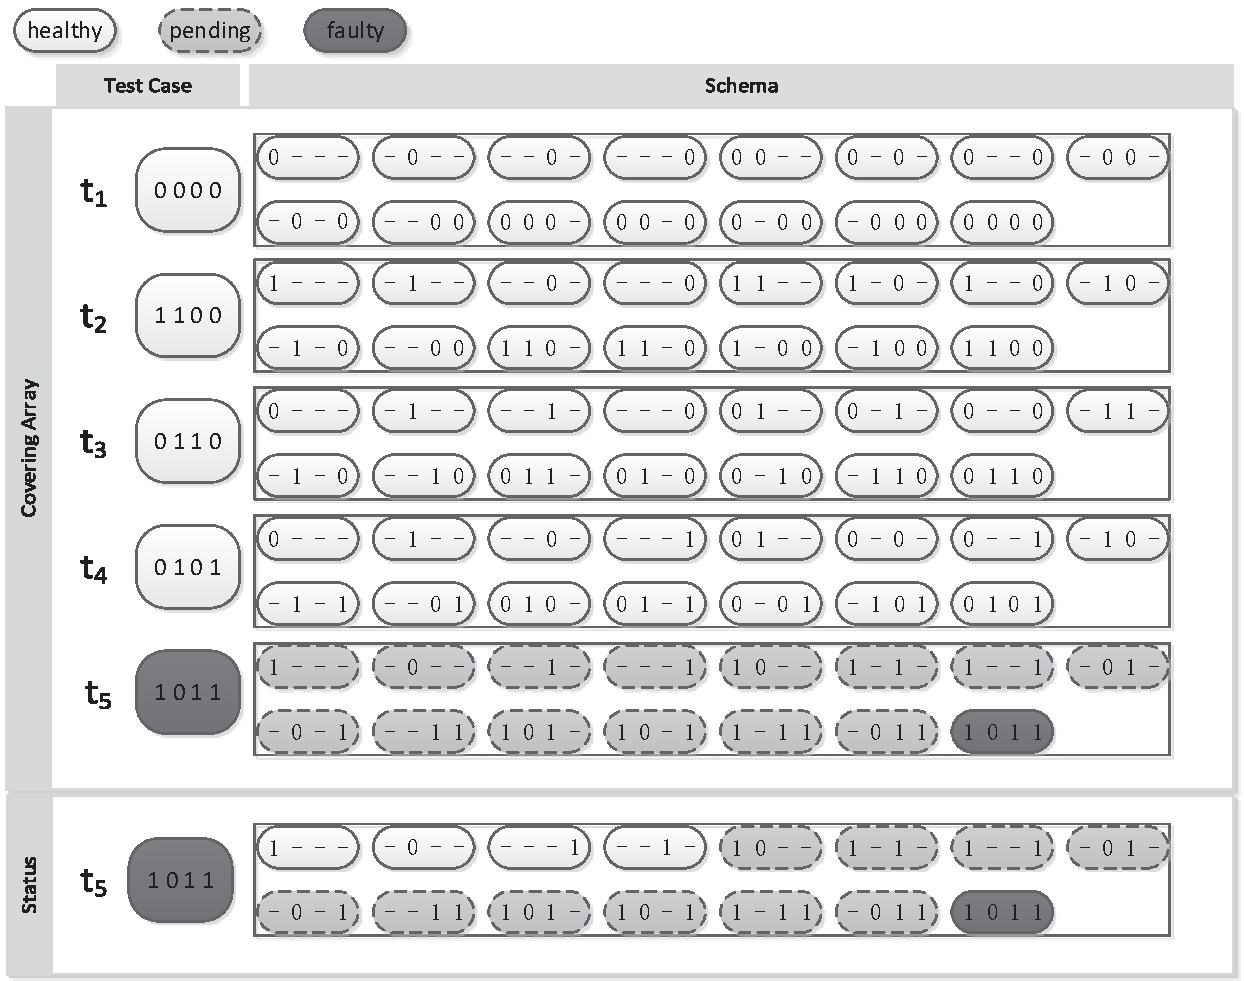
\includegraphics[width=5.6in]{ca.pdf}
 \caption{The incompleteness of Covering array }
 \label{fig_inc_ca}
\end{figure*}

In this figure, the test case with dark color represents a failing test case, while the test case with white color is a passing test case. The schema with white color is non-faulty, i.e., will not cause a failure, while the schema with dark color is faulty, i.e., any test case contain this schema would fail after testing. At last, the schema with light dark color and dashed outline is the pending schema, indicating that we cannot still determine whether it is faulty or non-faulty.

In this figure, we can first observe that all the schemas in the passing test case is non-faulty. This result is according to the first rule we mentioned before. The second observation is that the schema with the maximal number of factors (4 factors) in a failing test case is a faulty schema. In fact, this schema is the failing test case itself, i.e., (1, 1, 0, 1). This is because the failing test case must contain at least one MFS (otherwise, it will not fail). Hence, the schema which is the test case itself must also contain at least one MFS. As a result, it must be faulty schema according to the second rule we mentioned before. The last observation is that the other schemas in this failing test case $t_{5}$ are not guaranteed to be faulty schemas. In fact, if we assume this test case only contains one MFS (1, 1, 0, 1), then all the other schemas can be non-faulty schemas. Hence, these schemas cannot be determined to be faulty or not if we focus on this failing test case alone. As a result, we label these schemas as pending schemas initially.

Combining the three observations, we can further remove some pending schemas in $t_{5}$ by selecting the schemas that have already been appeared in the passing test cases. These schemas are (1, -, -, -), (-, -, 0, -), (-, 1, -, -), and (-, -, -, 0), which are labeled as non-faulty schemas. At last, the determination results of these schemas of $t_{5}$ can be shown in the ``\emph{Status}'' row. Note that except for these schemas that have been determined to be faulty and non-faulty, there still exist some pending schemas we cannot further removed by the original two rules. For example, (1, 0, -, -) didn't appear in any passing test case, and it did not contain any identified MFS. Hence, in this example, a single covering array is incomplete because of the existence of these pending schemas.

%because any schema can be the MFS in this test case. For example, if the test case itself as MFS, then no other schemas in this test case can be faulty schema.
%Initially. The schema with light dark color and dashed outline is the pending schema. These schemas cannot be determined by these two rules in the beginning. For example, schema (0, -, 1, -) is not appear in any passing test case, neither contain not any MFS.
%
%Initial is pending. Combining all the information, it is non-faulty.
%
%and the schema with
%
%In terms of making the failing test case clear. In this figure, which denoted what. what denoted what.

%\subsection{The incompleteness of error locating array}
%Since that , many approaches give a alleviation of how to compute the remaining schemas, which is called the fault localization. Error locating array is one of them. However, this time, we also give .

\subsection{The incompleteness of OFOT}
%SOFOT
Since covering array alone cannot remove all the pending schema in the failing test cases, we need more information to satisfy this target.  According to the second rule, i.e., the schema that contain the MFS is faulty schema, one method to reduce the number of pending schemas is to filter out those schemas which contain the MFS. However, without knowing the specific MFS in prior, we can only guarantee that the failing test case itself is faulty schema (it must contain the MFS). In fact, with the covering array alone, this is what we can only do to utilize the second rule.

Hence, to further reduce the set of pending schemas, we need to identify the MFS in the failing test case. One-Factor-One-Time (OFOT) \cite{nie2011minimal} is one of the most wildly used MFS identification approach. It identifies the MFS by modifying the original failing test case to see whether the modification would break the MFS in it. More specifically, at each time, it modifies one factor of the original failing test case and keeps the remaining factors to be as the same as the original failing test case. By doing this, it generates one new test case at each time. It then tests the newly generated test case. If this newly generated test case passes, it indicates the modified factor break the MFS in the original failing test case, and therefore, the original factor in the failing test case is one factor in the MFS. Otherwise, the original factor in the failing test case is not the factor in the MFS if the newly generated test case fails.
%Note that this conclusion is based on the newly generated MFS will not introduce new MFS, and hence, OFOT may not always obtain the accurate MFS.
%In fact, all the MFS identification approaches suffer from the need some assumptions to identify the MFS,

%which is also what we do in the covering arrays.
% For all we know is that the schemas as the failing test cases itself contain the MFS, others we do not know. Hence, it is important to identify the MFS to further narrow down the set of pending schemas.
Next, let us use OFOT to identify the MFS and help to narrow down the set of pending schemas of $t_{5}$ in the original covering array. First, we assume that there is one MFS (-, -, 1, 1) in failing test case $t_{5}$.  Then OFOT will work as follows: it generates four additional test cases $t_{6}$ to $t_{9}$ as shown in Figure \ref{fig_ofot_single}, respectively, each of which has one factor to be mutated from $t_{5}$.  Since $t_{8}$ and $t_{9}$ passed after testing, the original two factors (-, -, 1, -) and (-, -, -, 1) in $t_{5}$ are two factors in the MFS. The fails of $t_{6}$ and $t_{7}$ shows that there is no other factors in this MFS. Hence, OFOT identified the schema (-, -, 1, 1) as the MFS, which is identical to the schema (-, -, 1, 1) that we set as MFS in prior.

%MFS identification task is to distinguish. The wildly used approach is OFOT.
\begin{figure*}[ht]
 \centering
 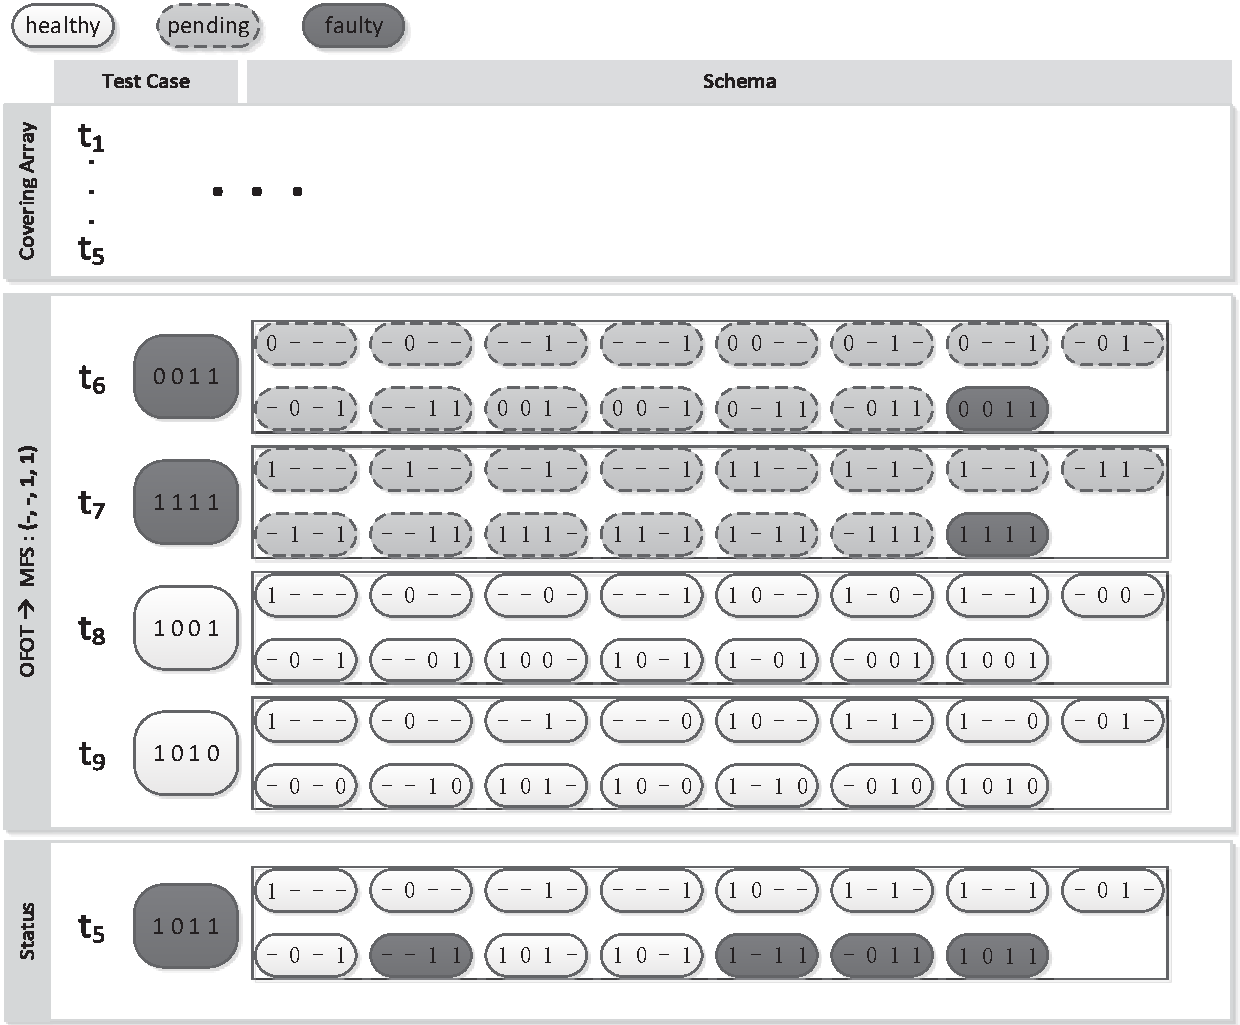
\includegraphics[width=5.6in]{ofot_single.pdf}
 \caption{OFOT with single MFS}
 \label{fig_ofot_single}
\end{figure*}

To analyse the pending schemas, we first list all the schemas in each additional test case in Figure \ref{fig_ofot_single}. The same as we observed from the covering array example, for the passing test case $t_{6}$ and $t_{7}$, all the schemas contained in it are non-faulty. For the failing test cases $t_{8}$ and $t_{9}$, we initially set the schemas which are failing test cases themselves as faulty schemas. Other schemas in these two failing test cases are all set to be pending schemas initially.

With these additional information, let us re-consider the status of the schemas in the original failing test case $t_{5}$. Firstly, as the identified MFS is (-, -, 1, 1), we can remove all the pending schemas of $t_{5}$ which contain this schema. These schemas are (-, -, 1, 1), (1, -, 1, 1), (-, 0, 1, 1), and (1, 0, 1, 1), respectively, and are labeled with dark color in the  ``\emph{Status}'' row for $t_{5}$ in Figure \ref{fig_ofot_single}. Next, we remove all the pending schemas of $t_{5}$ which appeared in these two passing test case $t_{6}$ and $t_{7}$. As shown in the  ``\emph{Status}'' row of Figure \ref{fig_ofot_single}, all the remaining pending schemas are removed and labeled with white color. Hence, we can learn that in this single MFS circumstance, OFOT works perfectly to remove all the pending schemas. However, when the failing test case contains multiple MFS, it does not go that well.

Now let us assume there are two MFS in the failing test case $t_{5}$, which are (1, 0, -, -) and (-, -, 1, 1), respectively. At this time, OFOT still generates the same four additional test cases, i.e., $t_{6}$ to $t_{9}$,  as shown in Figure \ref{fig_ofot_multi}. But different from the example of single MFS,  all the additional test cases failed at this time. This is because, the strategy of OFOT, i.e., mutating one factor at one time, cannot break all the MFS at the same time. As a result, it cannot identify any of the MFS.
%Why minimal failure-causing schema is not effective?
%This example shows that . Because there still existing pending schemas.
\begin{figure*}[ht]
 \centering
 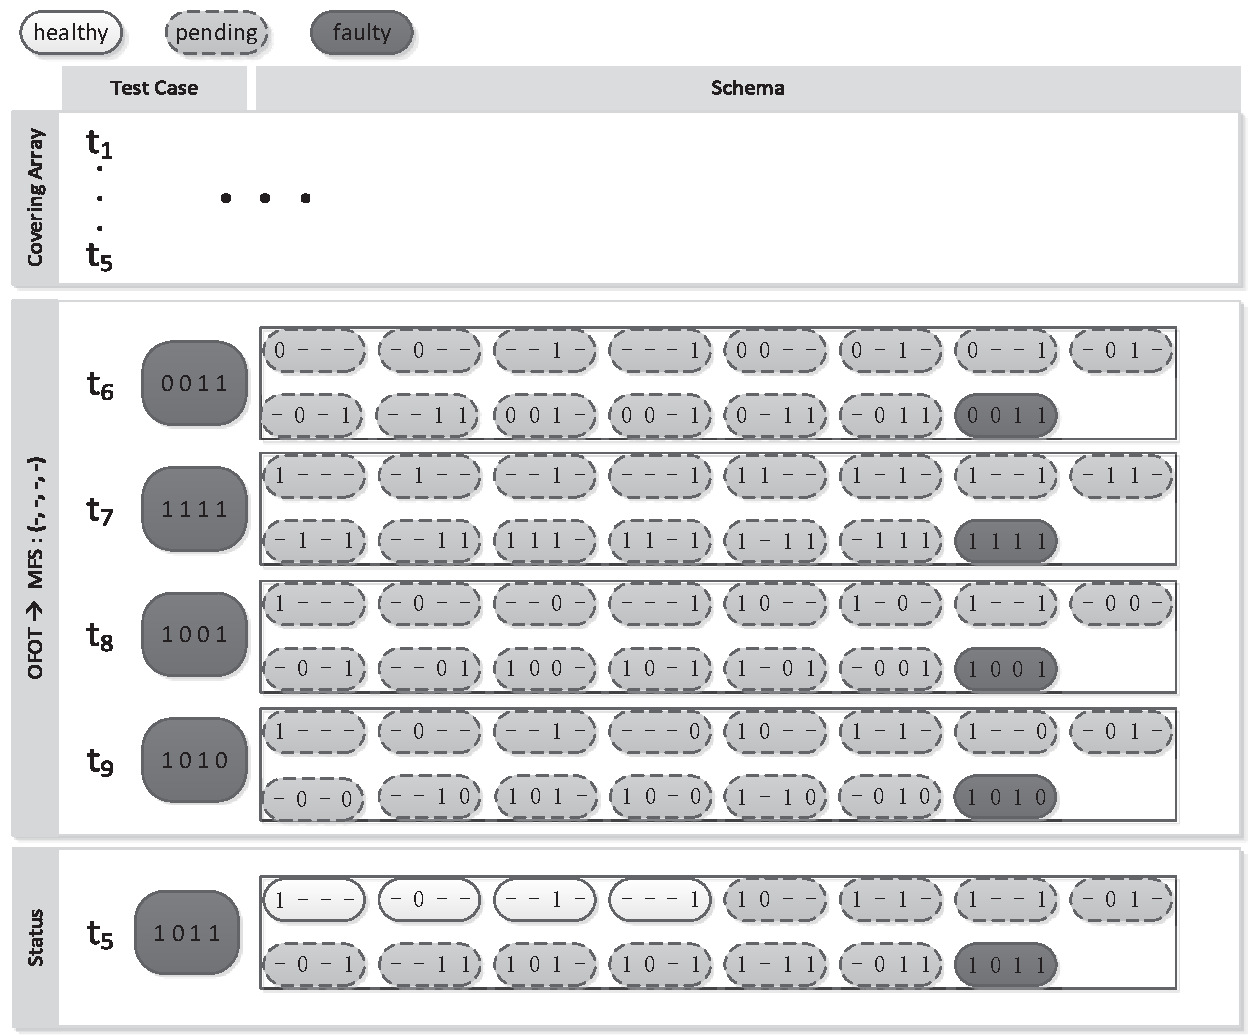
\includegraphics[width=5.6in]{ofot_multi.pdf}
 \caption{OFOT with multi MFS}
 \label{fig_ofot_multi}
\end{figure*}

There are two negative influences of this result. First, as we cannot identify the MFS by OFOT, the pending schemas in $t_{5}$ that contain the MFS also cannot be determined. Second, as all the test cases failed after testing, we cannot remove any pending schemas in $t_{5}$ that appear in the passing test case. As a result, the status of the pending schemas of $t_{5}$ will evolve to the ``\emph{Status}'' row of Figure \ref{fig_ofot_single}. We can observe that the status of the schemas of $t_{5}$ is the same as the previous example with only using covering array alone. Hence, in the condition that one failing test case contains multiple MFS, the MFS identification approach OFOT is still incomplete.


\subsection{The incompleteness of FIC}

From the example of OFOT, we can learn the main cause of incompleteness of OFOT is that the failing test case contains multiple MFS. For this, FIC \cite{zhang2011characterizing} (short for Faulty Interaction Characterization) augmented OFOT to handle the multiple MFS problem.
%It also mutates each factor in the original failing test case to generate additional test cases. But different from OFOT, which does not keep the value of the last mutation factor in the next test case generation (at each time, OFOT only mutates one factor and keep the remaining factors the same as the original failing test case), FIC may keep some changes in the next test case generation.  Specifically, when last generated test case failed after testing, FIC will keep the value of the changed factor to the next generations; Otherwise, if the last generated test case passed, FIC will not keep the value of the changed factor and assign the value of the original failing test case to this factor in the next generations. The reason for this is to  make FIC focus on only one MFS at each time and forbidden the appearance of other MFS.
FIC also mutates one factor at a time to generate one additional test case.  The only difference is that it will not always rollback to the original value of one factor it has mutated when it goes on mutating other factors (only when a passing test case appears, it will rollback to the original value). This operation will break multiple MFS in one test case and finally there remains only one MFS to identify. We still use the same example of multiple MFS used in OFOT to illustrate how FIC works and to see whether FIC satisfies the completeness criteria. The result is shown in Figure \ref{fig_fic_multi}.

\begin{figure*}[!htb]
 \centering
 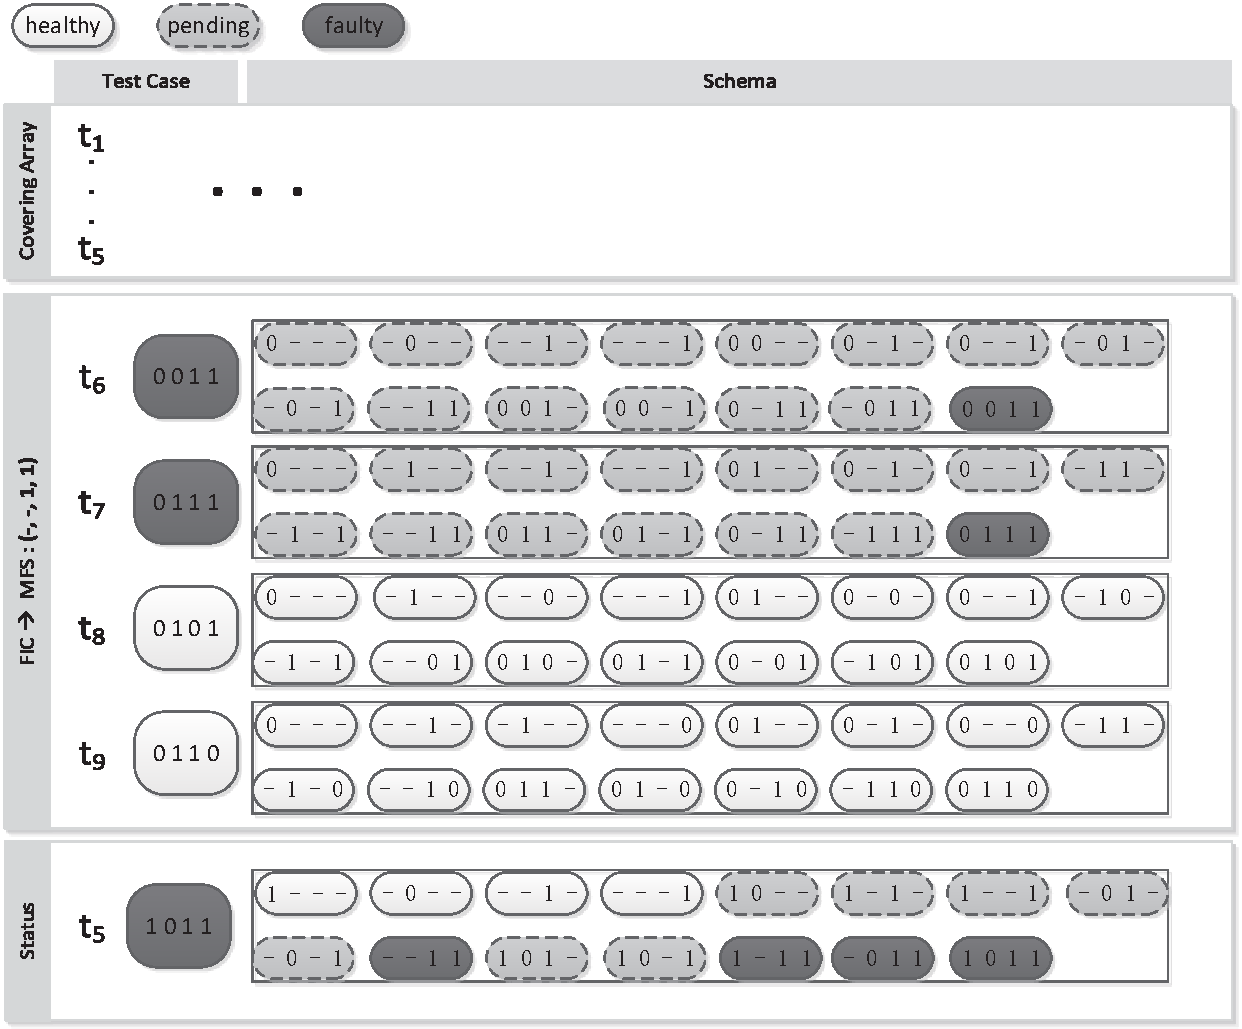
\includegraphics[width=5.3in]{fic.pdf}
 \caption{FIC with multiple MFS}
 \label{fig_fic_multi}
\end{figure*}

In Figure \ref{fig_fic_multi}, FIC also generated four additional test cases $t_{6}$ to $t_{9}$. The first case $t_{6}$ is the same as the $t_{6}$ generated by OFOT, but the second additional test case $t_{7}$ generated by FIC is different from $t_{7}$ generated by OFOT. This is because $t_{7}$ generated by FIC keeps the first value of $t_{6}$ (which is a failing test case) instead of the original first value of $t_{5}$. Note that FIC also keeps this value in the following generated test cases $t_{8}$ and $t_{9}$. By doing this, FIC forbids the appearance of the MFS (1, 0, -, -) later. The same as the first value of $t_{6}$, $t_{8}$ and $t_{9}$ keep the second value of $t_{7}$ because $t_{7}$ is also a failing test case. The failings of $t_{6}$ and $t_{7}$ indicated that there still exists other MFS in the original failing test case $t_{5}$, while the first and second factor is not in the remaining MFS.

With respect to the passing test case $t_{8}$, test case $t_{9}$ did not keep the third value of $t_{8}$ but rollback to the value of the original failing test case $t_{5}$. This is because, since $t_{8}$ passed after testing, there is no MFS in this test case. FIC should rollback this value to keep this factor of the MFS and check if there exists other factor of this MFS or not. After all, the passings of $t_{8}$ and $t_{9}$ indicated that (-, -, 1, -) and (-, -, -, 1) are two the factors in the remaining MFS. Hence, the MFS identified by FIC is (-, -, 1, 1).

Next, let us check status of the original failing test case $t_{5}$. The same as OFOT, we first remove the pending schemas that contain the MFS (-, -, 1, 1), and then remove the pending schemas that appear in the additional passing test case. The result is listed in the ``\emph{Status}'' row of Figure \ref{fig_fic_multi}. We can observe that there still exists 6 pending schemas, i.e., (1, 0, -, -), (1, -, 1, -), (1, -, -, 1), (1, 0, 1, -), (1, 0, -, 1), (-, 0, 1, -), and (-, 0, -, 1), respectively.

One reason for this incompleteness that FIC missed anther MFS in the failing test case $t_{5}$, which is (1, 0, -, -). The iterative version of FIC \cite{zhang2011characterizing}, i.e., FINOLP is designed to handle this problem. Specifically, after identifying one MFS in the original failing test case,  FINOLP first generates one more test case by mutating the factors in the original failing test case which appear in the identified MFS. If the generated test case fails after testing, which indicates that there still exists other MFS, it will use FIC to identify the MFS in this generated test case. This process repeats until the test case which is generated by mutating all the factors in the identified MFS passes. Figure \ref{fig_finovlp_multi} shows the detail when applying FINOLP on this example.
%The incompleteness of Finovlp

\begin{figure*}[!htb]
 \centering
 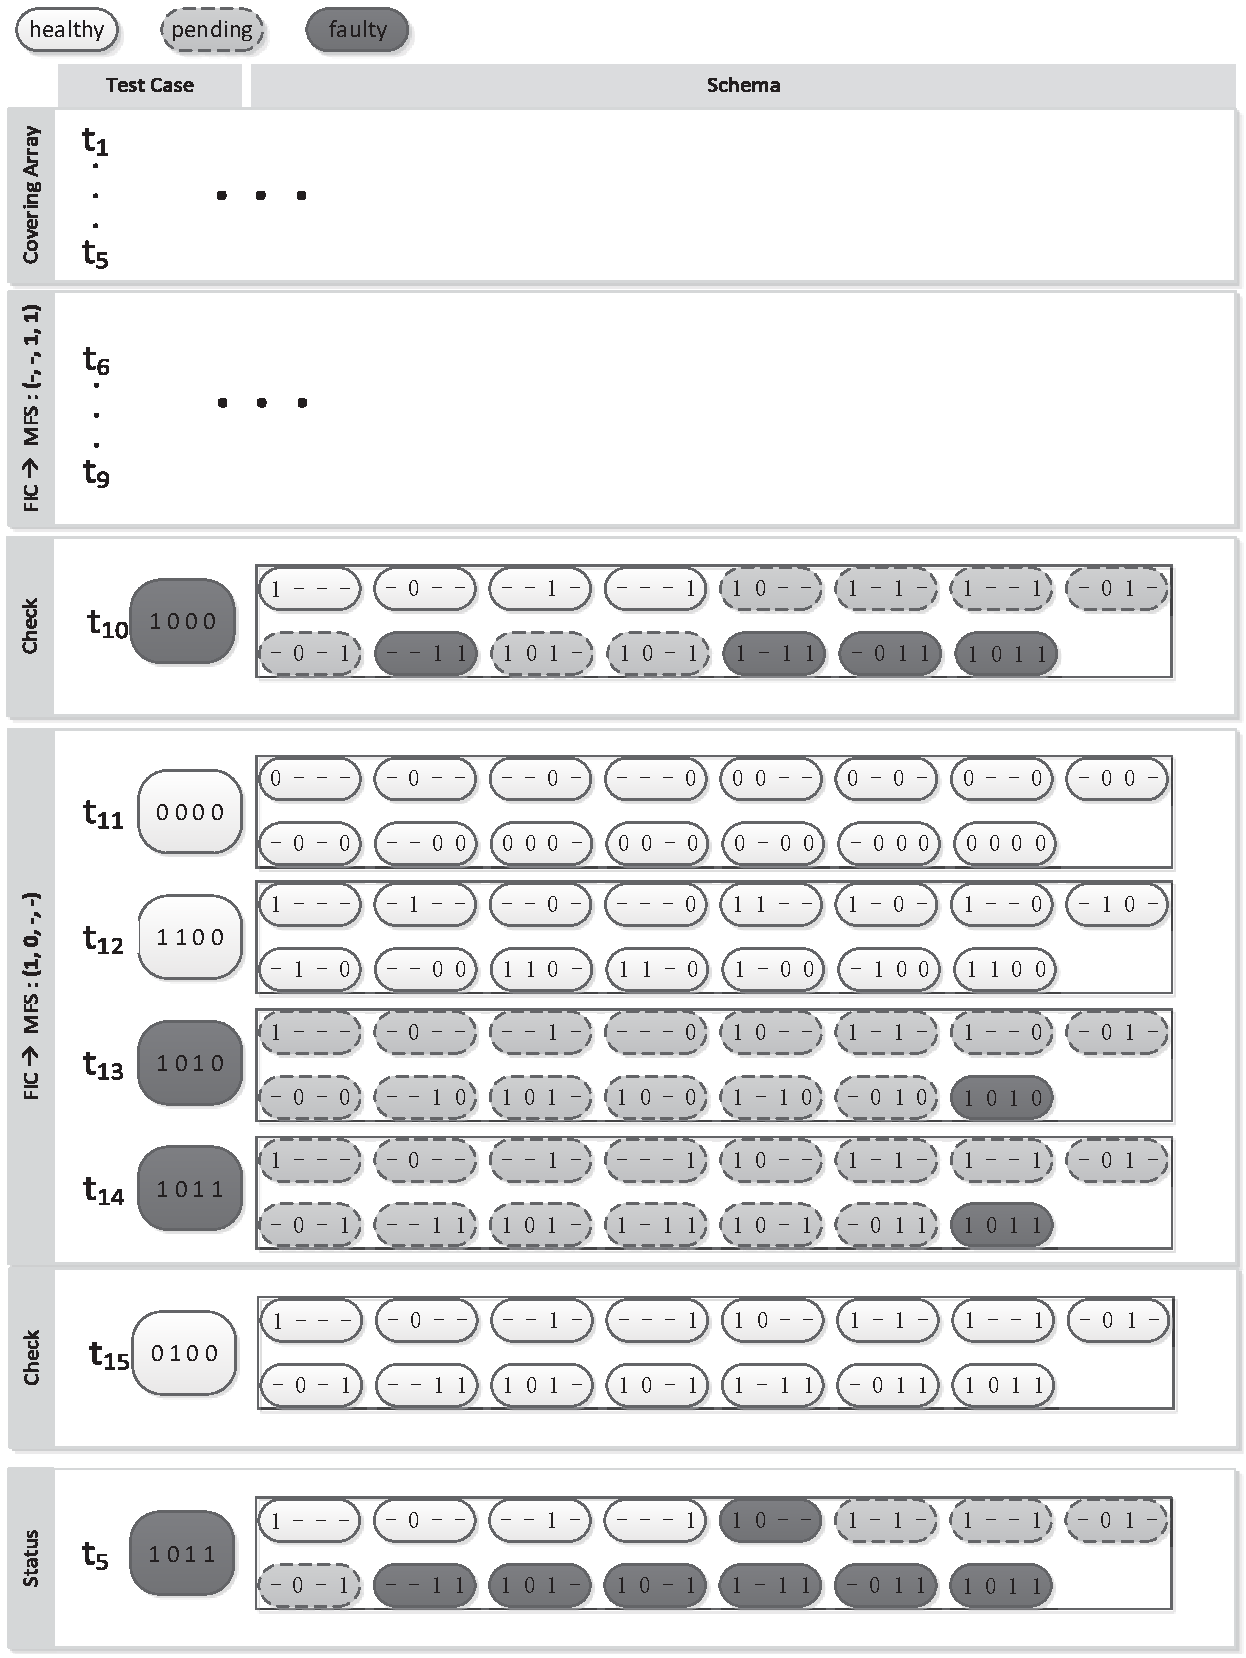
\includegraphics[width=5.3in]{finovlp.pdf}
 \caption{FINOVLP with multiple MFS}
 \label{fig_finovlp_multi}
\end{figure*}

In Figure \ref{fig_finovlp_multi}, test cases $t_{1}$ to $t_{9}$ are the same as those of the example in Figure \ref{fig_fic_multi}.  After identifying the MFS (-, -, 1, 1), FINOLP first generated the test case $t_{10}$ to check whether there exists other MFS in the original failing test case $t_{5}$ by mutating the values that appear in this MFS. Since $t_{10}$ failed after testing, it repeated FIC approach on $t_{10}$ to identified the remaining MFS. Therefore, it generated four additional test cases $t_{11}$ to $t_{14}$. The passings of $t_{11}$ and $t_{12}$ indicated another MFS was (1, 0, -, -). FINOLP continued to check whether there exists any other MFS by generating the test case $t_{15}$. The passing of $t_{15}$ showed that there did not exist any other MFS in the original failing test case $t_{5}$. Above all, FINOLP accurately identified all the MFS we have set in piror.

Next, the same as before, we use the two rules to check the status of the pending schemas in the original failing test case $t_{5}$. The result is shown in the ``\emph{Status}'' row of Figure \ref{fig_finovlp_multi}. We can observe that there still exists four schemas, which are (1, -, 1, -), (1, -, -, 1), (-, 0, 1, -), and (-, 0, -, 1), respectively. It is easy to find that these four schemas neither contain any MFS nor appears in any passing test cases. Hence, although FIC and FINOLP can handle the multiple MFS problem, it is still incomplete for the existence of these pending schemas.

\subsection{Additional efforts to remove the pending schemas}

Since Covering array, OFOT, FIC, and FINOLP cannot remove all the pending schemas, more efforts are needed to accomplish this goal. Note that to clear all the pending schemas is important, because some of them can be potential faulty schemas and may be harmful for this system under testing. For this, we decided to check these remaining pending schemas by generating more test cases that contained them and executing these test cases. If these test cases passes, we can directly use the first rule we mentioned before to determine these schemas to be non-faulty schemas. Otherwise, we need to adopt other methods to determine these schemas to be faulty or not.

\begin{figure*}[!htb]
 \centering
 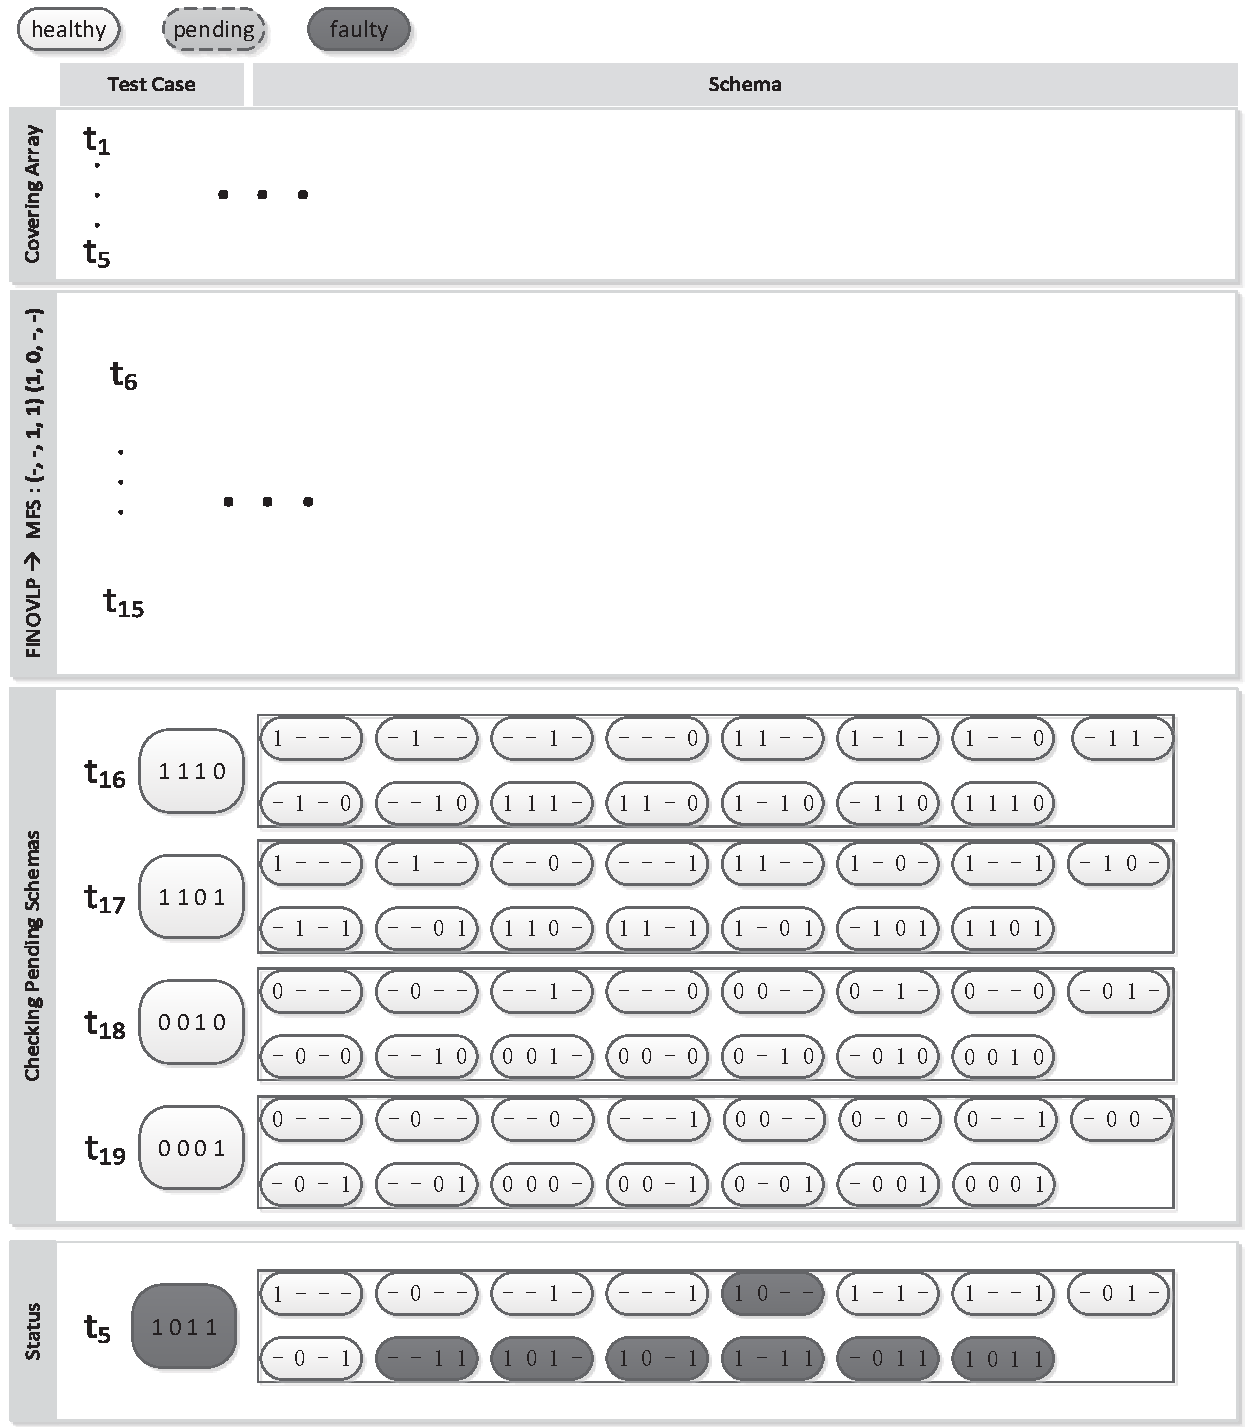
\includegraphics[width=5.3in]{non-pending.pdf}
 \caption{Additional efforts to remove pending schemas}
 \label{fig_no_pending}
\end{figure*}

As for this example, we generated four test cases to contain these pending schemas one by one (Note that in this example, we cannot generate one test case contain more than one pending schema without including any MFS). The result is shown in Figure \ref{fig_no_pending}. In this figure, all the additional test cases, i.e., $t_{16}$ to $t_{19}$, passed after testing. Hence, all the remaining schemas are non-faulty schemas. The final status of the pending schemas of $t_{5}$ is shown in the ``\emph{Status}'' row of Figure \ref{fig_no_pending}. We can observe that all the schemas in $t_{5}$ are determined to be non-faulty or faulty. Hence, in this condition, we can guarantee that the test of $t_{5}$ is complete.

Note that if any of the test case ($t_{16}$ to $t_{19}$) failed after testing, we cannot determine whether the corresponding pending schema in that test case is faulty or not.  In this case, we need to generate more test cases to determine the status of this pending schema (If this schema is a faulty schema, the cost will increase exponentially according to the formal definition of faulty schema which will be given later).

\subsection{A summary}

There are two main observations from this section. First, traditional covering array and MFS identification approaches are still incomplete in terms of the existence of pending schemas which cannot be determined to faulty or non-faulty. Second, to remove all the pending schemas is time-consuming. In fact, just listing all the schemas and checking them one by one is inefficient. In this example, we need to check $2^{4} - 1 = 5$ schemas for each test case. However, with the increase of the number of factors in one test case, the cost for checking the pending schemas increase exponentially.

For all of these, we need to theoretically analyze the properties of the pending schemas in the failing test cases and to give a more efficient method to obtain them.
%It needs a formal definition and theoretical analysis for the pending schemas with non-faulty schemas and faulty schemas.

\section{Background}\label{sec:back}
This section presents some definitions and propositions to give a formal model for CT.
%\subsection{Failure-inducing interactions in CT}
Without loss of generality, assume that the Software Under Test (SUT) is influenced by a set of parameters $P$, which contains \emph{n} parameters, and each parameter $p_{i} \in P$ can take the values from the finite set $V_{i}$ ($i$ = 1,2,..n).

\newtheorem{assumption}{Assumption}

\subsection{Test cases and schemas}\label{sec:back:testandschema}
In this subsection, we will formally define the test case and schema. We will also give the properties to reveal the relationships between them. In these propositions, Proposition   are originated from our previous work .
 %Moreover, we will use the same SUT in the motivation (the MS-WORD example that has four factors may influnence  ) to show the definitions and propositions.

\begin{definition}\label{de:testcase}
A \emph{test case} of the SUT is a tuple of \emph{n} values, one for each parameter of the SUT. It is denoted as  ($v_{1}$, $v_{2}$,...,$v_{n}$), where $v_{1}\in V_{1}$, $v_{2} \in V_{2}$ ... $v_{n} \in V_{n}$.
\end{definition}

In practice, these parameters in the test case can represent many factors, such as input variables, run-time options, building options or various combination of them. We need to execute the SUT with these test cases to ensure the correctness of the behaviour of the SUT.

\begin{definition}\label{de:schema}
For the SUT, the $\tau$-set \{$(p_{x_{1}}, v_{x_{1}})$, $(p_{x_{2}}, v_{x_{2}})$, ..., $(p_{x_{\tau}}, v_{x_{\tau}})$\}, where $0 \leq x_{i} \leq n$, $p_{x_{i}} \in P$, and $v_{x_{i}} \in V_{x_{i}}$, is called a $\tau$-degree \emph{schema} ($0 < \tau \leq n $), when a set of $\tau$ values assigned to $\tau$ distinct parameters.
\end{definition}

For example, the interactions (Highlight: Off, Status Bar: On, Smart tags: Off) appearing in Section \ref{sec:intro} is a 3-degree schema, where three parameters are assigned to corresponding values. In effect a test case itself is a n-degree \emph{schema}, which can be described as \{$(p_{1}, v_{1})$, $(p_{2}, v_{2})$, ..., $(p_{n}, v_{n})$\}. Also, for any schema, say, $s$, its degree can be denoted as $|s|$ because a schema is essentially  a set of parameter values.

Note that this definition of schema is a formal description of schemas we discussed in the section of \emph{Motivation}. For example, the schema (1, -, 0, -) is exactly the schema \{ $(p_{1}, 1)$, $(p_{3}, 0)$ \} here. We use this formal definition because it benefits the description of the following theoretical analysis, including these propositions and proofs.

\begin{definition}\label{de:subsume}
Let $s_{1}$, $s_{2}$ be two schemas in SUT. If $\forall (p_{x_{1}}, v_{x_{1}}) \in s_{1}$, $(p_{x_{1}}, v_{x_{1}}) \in s_{2}$, then $s_{1}$ is the $sub-schema$ of $s_{2}$, and $s_{2}$ the $super-schema$ of $s_{1}$, which can be denoted as $s_{1} \preceq s_{2}$. Further, if $|s_{1}| < |s_{2}|$, we call $s_{1}$ the $real-sub-schema$ of $s_{2}$, which is denoted as $s_{1} \prec s_{2}$.
\end{definition}

For example,  the 2-degree schema \{($p_{1}, 1$), ($p_{2}, 0$)\} is a sub-schema (also is a real-sub-schema) of the 3-degree schema \{($p_{1}, 1$), ($p_{2}, 0$), ($p_{4}, 1$)\}.
%Also, since a test case itself is a schema, then if a test case $t$ contains a schema $s$, we have $s \preceq t$. For example,  the 2-degree schema \{($p_{1}, 1$), ($p_{2}, 0$)\} is also a sub-schema of a test case \{($p_{1}, 1$), ($p_{2}, 0$), ( Bookmarks, On), ($p_{4}, 1$)\}.

According to the definition of schemas, it is easy to find the following three properties of schemas.

\begin{proposition}[Reflexivity]\label{pro:subsumereflexivity}
For any schema $s$, $s \preceq s$.
\end{proposition}

\begin{proof}
Since $\forall (p_{x_{i}}, v_{x_{i}})\in s$, $(p_{x_{i}}, v_{x_{i}}) \in s$. Hence, $s \preceq s$ according to the definition of \ref{de:subsume}.
\end{proof}

This proposition tells that any schema is the subschema of itself. For example the 2-degree schema \{($p_{1}, 1$), ($p_{2}, 0$)\} is a sub-schema of itself  \{($p_{1}, 1$), ($p_{2}, 0$)\}.

\begin{proposition}[Antisymmetry]\label{pro:subsumeantisymmetry}
For schemas $s_{1}$, $s_{2}$, if $s_{1} \preceq s_{2}$ and $s_{2} \preceq  s_{1}$, then $s_{1}$ = $s_{2}$.
\end{proposition}

\begin{proof}
As $s_{1} \preceq s_{2}$, then $\forall (p_{x_{i}}, v_{x_{i}})\in s_{1}, (p_{x_{i}}, v_{x_{i}}) \in s_{2}$. This indicates that the parameter value set $s_{1}$ is the subset of  $s_{2}$, i.e., $s_{1} \subseteq s_{2}$.  Also as $s_{2} \preceq s_{1}$, $s_{2} \subseteq s_{1}$. Since, $s_{1} \subseteq s_{2}$ and $s_{2} \subseteq s_{1}$, we have the two parameter value sets $s_{1}$ and $s_{2}$ are equal, i.e., $s_{1}$ = $s_{2}$.
\end{proof}

This proposition shows that for two distinct schemas, one cannot be both super-schema and sub-schema of the other schema. For example, the 2-degree schema \{($p_{1}, 1$), ($p_{2}, 0$)\} is a sub-schema of the 3-degree schema \{($p_{1}, 1$), ($p_{2}, 0$), ($p_{4}, 1$)\}, but not a super-schema of this 3-degree schema.  Only two equal schemas can be both the sub-schema and super-schema of each other. For example, the 2-degree schema \{($p_{1}, 1$), ($p_{2}, 0$)\} is both the sub-schema and super-schema of itself.
%related in both directions.

\begin{proposition}[Transitive]\label{pro:subsumetrans}
Given schemas $s_{1}$, $s_{2}$, and $s_{3}$, if $s_{1} \preceq s_{2}$, $s_{2} \preceq s_{3}$, then $s_{1} \preceq s_{3}$.
\end{proposition}

\begin{proof}
As $s_{1} \preceq s_{2}$, then $\forall (p_{x_{i}}, v_{x_{i}})\in s_{1}, (p_{x_{i}}, v_{x_{i}}) \in s_{2}$. Also, $s_{2} \preceq s_{3}$, then $\forall (p_{x_{i}}, v_{x_{i}})\in s_{2}, (p_{x_{i}}, v_{x_{i}}) \in s_{3}$. Hence, $\forall (p_{x_{i}}, v_{x_{i}})\in s_{1}, (p_{x_{i}}, v_{x_{i}}) \in s_{3}$. According to definition \ref{de:subsume}, $s_{1} \preceq s_{3}$.
\end{proof}

This proposition shows the transitivity of the subsuming relationships of schemas. For example, the 1-degree schema \{($p_{1}, 1$)\} is a sub-schema of the 2-degree schema \{($p_{1}, 1$), ($p_{2}, 0$)\}, and this 2-degree schema is a sub-schema of the 3-degree schema \{($p_{1}, 1$), ($p_{2}, 0$), ($p_{4}, 1$)\}. Therefore, the 1-degree schema \{($p_{1}, 1$)\} is also a sub-schema of the 3-degree schema \{($p_{1}, 1$), ($p_{2}, 0$), ($p_{4}, 1$)\}.


These three propositions together show that the schema set $(s, \preceq)$ is a partial order set. Next, we will introduce the relationships between schemas and tests.

\begin{definition}\label{de:containorhit}
For a schema $s$, if there exists one test case $t$, such that each parameter value in the schema $s$ is also in the test case $t$, i.e., $\forall (p_{x_{i}}, v_{x_{i}}) \in s, (p_{x_{i}}, v_{x_{i}}) \in t$, then we call the test case $t$ \emph{hits} or \emph{contains} the schema $s$, and test case $t$ is one \emph{container} of schema $s$.
\end{definition}

Note that test case is also a $n$-degree schema, hence when a test case $t$ hits one schema $s$, we can denote this relationship simply as $s \preceq t, |t| = n$. As an example, test case \{($p_{1}, 1$), ($p_{2}, 0$), ($p_{3}, 1$), ($p_{4}, 0$)\} hits the 2-degree schema \{($p_{1}, 1$), ($p_{2}, 0$)\}.

\begin{definition} \label{de:alltests}
 For a schema $s$, the set of all the possible containers of it, i.e., the set of all the possible test cases that contain this schema, is called the \emph{whole set} of containers of this schema $s$, which is denoted as $\mathcal{T}(s)$.
\end{definition}

Formally, $\mathcal{T}(s) = \{ t | s \preceq t, |t| = n\}$. As an example, let us consider the SUT that has four parameters and each parameter has two values (All the following examples are based on the same SUT). Let schema $s$ be \{($p_{1}, 1$), ($p_{2}, 0$)\}. Table \ref{ex:wholecontainer} shows $\mathcal{T}(s)$.  It can be observed that each possible test case in the SUT that contains schema $s$ is listed in Table \ref{ex:wholecontainer}.
 %are the set of four test cases \{ \{($p_{1}, 1$), ($p_{2}, 0$), ($p_{3}, 0$), ($p_{4}, 0$)\}, \{($p_{1}, 1$), ($p_{2}, 0$), ($p_{3}, 0$), ($p_{4}, 1$)\} ,  \{($p_{1}, 1$), ($p_{2}, 0$), ($p_{3}, 1$), ($p_{4}, 0$)\}, \{($p_{1}, 1$), ($p_{2}, 0$), ($p_{3}, 1$), ($p_{4}, 1$)\}  \}.


\begin{table}[htbp]
  \centering
  \caption{Whole set of containers of \{($p_{1}, 1$), ($p_{2}, 0$)\}}
   % {\footnotesize
  \label{ex:wholecontainer}
    \begin{tabular}{|c|c|}\hline
  \multicolumn{2}{|c|}{ \textbf{Schema}} \\ \hline
   $s$ & \{($p_{1}, 1$), ($p_{2}, 0$)\} \\ \hline
  \multicolumn{2}{|c|}{ \textbf{ $\mathcal{T}(s)$ }}\\ \hline
    $t_{1}$ &   \{($p_{1}, 1$), ($p_{2}, 0$), ($p_{3}, 0$), ($p_{4}, 0$)\} \\
    $t_{2}$ &   \{($p_{1}, 1$), ($p_{2}, 0$), ($p_{3}, 0$), ($p_{4}, 1$)\} \\
    $t_{3}$ &   \{($p_{1}, 1$), ($p_{2}, 0$), ($p_{3}, 1$), ($p_{4}, 0$)\} \\
    $t_{4}$ &   \{($p_{1}, 1$), ($p_{2}, 0$), ($p_{3}, 1$), ($p_{4}, 1$)\} \\ \hline
    \end{tabular}
   % }
\end{table}%



With respect the the whole set of containers of one schema, we have the following property.

\begin{proposition}[{smaller schema has a larger $\mathcal{T}(s)$}] \label{pro:shl}
For schemas $s_{1}$ and $s_{2}$, if $s_{1} \preceq s_{2}$, then $\mathcal{T}(s_{2}) \subseteq \mathcal{T}(s_{1})$.
\end{proposition}

\begin{proof}
$\forall t \in \mathcal{T}(s_{2})$, $s_{2} \preceq t$. Since $s_{1} \preceq s_{2}$, we have $s_{1} \preceq t$ according to Proposition \ref{pro:subsumetrans}. That is, $t$ contains $s_{1}$. Therefore, $t \in \mathcal{T}(s_{1})$.  Hence,  $\mathcal{T}(s_{2}) \subseteq \mathcal{T}(s_{1})$.
\end{proof}

% Table generated by Excel2LaTeX from sheet 'T(s)'
As an example, let schema $s_{1}$ be \{($p_{1}, 1$), ($p_{2}, 0$)\}, and schema $s_{2}$ be \{($p_{1}, 1$), ($p_{2}, 0$), ($p_{3}, 0$)\}, which is one of the super-schemas of $s_{1}$. Table \ref{ex:smallerschemahaslarger} shows the whose set of containers of  $s_{1}$ and $s_{2}$. We can observe that $\mathcal{T}(s_{1})$ subsumes  $\mathcal{T}(s_{2})$.

\begin{table}[htbp]
  \centering
  \caption{Comparison of the whole set of containers of two subsuming schemas}
 %   {\footnotesize
      \label{ex:smallerschemahaslarger}
    \begin{tabular}{|c|c|} \hline
   \multicolumn{2}{|c|}{\textbf{Schema}} \\ \hline
   $s_{1}$ & \{($p_{1}, 1$), ($p_{2}, 0$)\} \\ \hline
   \multicolumn{2}{|c|}{\textbf{ $\mathcal{T}(s_{1})$ }}\\ \hline
   $t_{1}$ & \{($p_{1}, 1$), ($p_{2}, 0$), ($p_{3}, 0$), ($p_{4}, 0$)\} \\
   $t_{2}$ & \{($p_{1}, 1$), ($p_{2}, 0$), ($p_{3}, 0$), ($p_{4}, 1$)\} \\
   $t_{3}$ & \{($p_{1}, 1$), ($p_{2}, 0$), ($p_{3}, 1$), ($p_{4}, 0$)\} \\
   $t_{4}$ & \{($p_{1}, 1$), ($p_{2}, 0$), ($p_{3}, 1$), ($p_{4}, 1$)\} \\ \hline\hline
   \multicolumn{2}{|c|}{ \textbf{ Schema}} \\ \hline
   $s_{2}$ & \{($p_{1}, 1$), ($p_{2}, 0$), ($p_{3}, 0$)\} \\ \hline
   \multicolumn{2}{|c|}{\textbf{ $\mathcal{T}(s_{2})$ }}\\ \hline
   $t_{1}$ & \{($p_{1}, 1$), ($p_{2}, 0$), ($p_{3}, 0$), ($p_{4}, 0$)\} \\
   $t_{2}$ & \{($p_{1}, 1$), ($p_{2}, 0$), ($p_{3}, 0$), ($p_{4}, 1$)\} \\ \hline
    \end{tabular}%
   % }
\end{table}%



\begin{definition} \label{de:allschemas}
For a test case $t$, all the schemas that it can hit is called the \emph{whole set} of hit schemas of $t$, which is denoted as $\mathcal{I}(t)$.
\end{definition}

Formally,$\mathcal{I}(t) = \{ s | s \preceq t \}$. As an example, let test case $t$ be  \{($p_{1}, 1$), ($p_{2}, 0$), ($p_{3}, 0$), ($p_{4}, 0$)\}. Table \ref{ex:wholesetofhitschemas} shows $\mathcal{I}$ ($t$). We can find it is a set of $2^{4} - 1 = 15$ schemas.

\begin{table}[htbp]
  \centering
  \caption{An example of whole set of hit schemas of one test case}
 %   {\footnotesize
      \label{ex:wholesetofhitschemas}
    \begin{tabular}{|c|c|} \hline
   \multicolumn{2}{|c|}{\textbf{Test Case}} \\ \hline
   $t$ & \{($p_{1}, 1$), ($p_{2}, 0$), ($p_{3}, 0$), ($p_{4}, 0$)\} \\ \hline
    \multicolumn{2}{|c|}{\textbf{ $\mathcal{I}(t)$ }}\\ \hline
   $s_{1}$ & \{($p_{1}, 1$)\} \\
   $s_{2}$ & \{($p_{2}, 0$)\} \\
   $s_{3}$ & \{($p_{3}, 0$)\} \\
   $s_{4}$ & \{($p_{4}, 0$)\} \\
   $s_{5}$ & \{($p_{1}, 1$),($p_{2}, 0$)\} \\
   $s_{6}$ & \{($p_{1}, 1$),($p_{3}, 0$)\} \\
   $s_{7}$ & \{($p_{1}, 1$),($p_{4}, 0$)\} \\
   $s_{8}$ & \{($p_{2}, 0$),($p_{3}, 0$)\} \\
   $s_{9}$ & \{($p_{2}, 0$),($p_{4}, 0$)\} \\
   $s_{10}$ & \{($p_{3}, 0$),($p_{4}, 0$)\} \\
   $s_{11}$ & \{($p_{1}, 1$),($p_{2}, 0$),($p_{3}, 0$)\} \\
   $s_{12}$ & \{($p_{1}, 1$),($p_{2}, 0$),($p_{4}, 0$)\} \\
   $s_{13}$ & \{($p_{1}, 1$),($p_{3}, 0$),($p_{4}, 0$)\} \\
   $s_{14}$ & \{($p_{2}, 0$),($p_{3}, 0$),($p_{4}, 0$)\} \\
   $s_{15}$ & \{($p_{1}, 1$), ($p_{2}, 0$), ($p_{3}, 0$), ($p_{4}, 0$)\} \\ \hline
    \end{tabular}%
   % }
\end{table}%


\begin{definition} \label{de:allschemasoft}
For a set of test case $T$, all the schemas that these test cases can hit is called the \emph{whole set} of hit schemas of $T$, which is denoted as $\mathcal{I}(T)$.
\end{definition}

$\mathcal{I}(T)$ extends $\mathcal{I}(t)$ to a set of test cases. Formally, $\mathcal{I}(T) = \bigcup_{t \in T} \mathcal{I}(t)$.


\begin{definition} \label{de:specialschema}
All the schemas that are \textbf{only} contained in test set $T$ is called the \emph{special schemas} of test case set $T$, which is denoted as  $\mathcal{S}(T)$.
\end{definition}

Formally, $\mathcal{S}(T) =  \mathcal{I}(T) \backslash \mathcal{I}(\bar{T}) $, where $\bar{T}$ is the complementary test set of $T$, i.e., $T \bigcup \bar{T} = T^{*}, T \bigcup \bar{T} = \emptyset$. Here, $T^{*}$ indicates all the possible test cases in the SUT. Based on this formula, we can learn that the special schemas are essentially the whole set of hit schemas of test case $T$, except for those hit schemas of other test cases.

As an example, let test case $t_{1}$ be \{($p_{1}, 1$), ($p_{2}, 0$), ($p_{3}, 0$), ($p_{4}, 0$)\} and $t_{2}$ be \{($p_{1}, 1$), ($p_{2}, 0$), ($p_{3}, 0$), ($p_{4}, 1$)\}. Let the test case set $T$ be \{ $t_{1}$ , $t_{2}$ \}. Table \ref{ex:specialschemasoftestset} shows the schemas of $\mathcal{S}(T)$. We can observe that there are only three schemas $s_{1}$, $s_{2}$, and $s_{3}$ in this schema set. Other hit schemas of $T$ that can appear in other test cases do not belong to $\mathcal{S}(T)$. For example, schema \{($p_{1}, 1$), ($p_{2}, 0$)\} can appear in the test case \{($p_{1}, 1$), ($p_{2}, 0$), ($p_{3}, 1$), ($p_{4}, 1$)\}, which is not in $T$. Hence, \{($p_{1}, 1$), ($p_{2}, 0$)\} is only one hit schema of $T$, but not the special schema of $T$.

\begin{table}[htbp]
  \centering
  \caption{An example of special schemas of test case set}
 %   {\footnotesize
      \label{ex:specialschemasoftestset}
    \begin{tabular}{|c|c|} \hline
  \multicolumn{2}{|c|}{\textbf{Test Case set $T$}} \\ \hline
  $t_{1}$ & \{($p_{1}, 1$), ($p_{2}, 0$), ($p_{3}, 0$), ($p_{4}, 0$)\}\\
  $t_{2}$ & \{($p_{1}, 1$), ($p_{2}, 0$), ($p_{3}, 0$), ($p_{4}, 1$)\}\\ \hline
  \multicolumn{2}{|c|}{\textbf{ $\mathcal{S}(T)$ }}  \\ \hline
  $s_{1}$ & \{($p_{1}, 1$), ($p_{2}, 0$), ($p_{3}, 0$)\}  \\
  $s_{2}$ & \{($p_{1}, 1$), ($p_{2}, 0$), ($p_{3}, 0$), ($p_{4}, 0$)\} \\
  $s_{3}$ & \{($p_{1}, 1$), ($p_{2}, 0$), ($p_{3}, 0$), ($p_{4}, 1$)\} \\ \hline
    \end{tabular}%
   % }
\end{table}%


With respect to the special schema set of test case $T$, we can obtain the following property.

\begin{proposition}[Whole container of special schema set]\label{pro:stct}
For any test set $T$ of the SUT,  $\bigcup_{s \in \mathcal{S}(T)}\mathcal{T}(s) = T$.
\end{proposition}
\begin{proof}
As $\mathcal{S}(T) =  \mathcal{I}(T) \backslash \mathcal{I}(\bar{T}) $,  $\forall s \in \mathcal{S}(T),\ s \in \mathcal{I}(T)\ and\ s \not\in \mathcal{I}(\bar{T})$. Then $\forall t \in \mathcal{T}(s), t \ contains\ s$, indicating that $t \in T$.  Hence, $\mathcal{T}(s) \subseteq T$.  Then $\bigcup_{s \in \mathcal{S}(T)}\mathcal{T}(s) \subseteq T$.

On the other hand, $\forall t \in T$,  $\exists s' \in \mathcal{I}(t)$, such that $s' \not\in \mathcal{I}(\bar{T})$ (at least it holds when $s' = t$). Hence, $s' \in \mathcal{S}(T)$.  Obviously $t \in \mathcal{T}(s') \subseteq \bigcup_{s \in \mathcal{S}(T)} \mathcal{T}(s)$. Therefore,  $ T \subseteq \bigcup_{s \in \mathcal{S}(T)}\mathcal{T}(s)$.

Since $\bigcup_{s \in \mathcal{S}(T)}\mathcal{T}(s) \subseteq T$ and $T \subseteq \bigcup_{s \in \mathcal{S}(T)}\mathcal{T}(s)$, we have $\bigcup_{s \in \mathcal{S}(T)}\mathcal{T}(s) =  T$.
\end{proof}


Proposition \ref{pro:stct} revels the relationship between test case set and its special schemas. That is, for a specific test set, the whole set of containers of its special schemas are equal to this original test set. As an example,
 let test case $t_{1}$, $t_{2}$  still be \{($p_{1}, 1$), ($p_{2}, 0$), ($p_{3}, 0$), ($p_{4}, 0$)\}, \{($p_{1}, 1$), and ($p_{2}, 0$), ($p_{3}, 0$), ($p_{4}, 1$)\}, respectively. Let the test case set $T$ be \{ $t_{1}$ , $t_{2}$\}.  Table \ref{ex:prospecialschemasoftestset} specifically shows the whole set of containers for each special schema for test case set $T$, as well as their union. We can observe that their union, i.e.,  $\bigcup_{s \in \mathcal{S}(T)}\mathcal{T}(s)$ is equal to the original test set $T$.

\begin{table}[htbp]
  \centering
  \caption{An example of the whole set of containers of special schemas}
 %   {\footnotesize
      \label{ex:prospecialschemasoftestset}
    \begin{tabular}{|c|c|} \hline
  \multicolumn{2}{|c|}{\textbf{Test Case set}} \\ \hline
  $t_{1}$ & \{($p_{1}, 1$), ($p_{2}, 0$), ($p_{3}, 0$), ($p_{4}, 0$)\}\\
  $t_{2}$ & \{($p_{1}, 1$), ($p_{2}, 0$), ($p_{3}, 0$), ($p_{4}, 1$)\}\\ \hline
  \multicolumn{2}{|c|}{\textbf{ $\mathcal{S}(T)$ }}  \\ \hline
  $s_{1}$ & \{($p_{1}, 1$), ($p_{2}, 0$), ($p_{3}, 0$)\}  \\
  $s_{2}$ & \{($p_{1}, 1$), ($p_{2}, 0$), ($p_{3}, 0$), ($p_{4}, 0$)\} \\
  $s_{3}$ & \{($p_{1}, 1$), ($p_{2}, 0$), ($p_{3}, 0$), ($p_{4}, 1$)\} \\ \hline
   \multicolumn{2}{|c|}{\textbf{ $\mathcal{T}(s_{1})$}}  \\ \hline
  $t_{1}$ & \{($p_{1}, 1$), ($p_{2}, 0$), ($p_{3}, 0$), ($p_{4}, 0$)\} \\
  $t_{2}$ & \{($p_{1}, 1$), ($p_{2}, 0$), ($p_{3}, 0$), ($p_{4}, 1$)\} \\ \hline
      \multicolumn{2}{|c|}{\textbf{ $\mathcal{T}(s_{2})$}}  \\ \hline
  $t_{1}$ & \{($p_{1}, 1$), ($p_{2}, 0$), ($p_{3}, 0$), ($p_{4}, 0$)\} \\ \hline
      \multicolumn{2}{|c|}{\textbf{ $\mathcal{T}(s_{3})$}}  \\ \hline
  $t_{2}$ & \{($p_{1}, 1$), ($p_{2}, 0$), ($p_{3}, 0$), ($p_{4}, 1$)\} \\ \hline
    \multicolumn{2}{|c|}{\textbf{  $\bigcup_{s \in \mathcal{S}(T)}\mathcal{T}(s)$ = $\mathcal{T}(s_{1}) \bigcup \mathcal{T}(s_{2}) \bigcup\mathcal{T}(s_{3})$ }}  \\ \hline
  $t_{1}$ & \{($p_{1}, 1$), ($p_{2}, 0$), ($p_{3}, 0$), ($p_{4}, 0$)\} \\
  $t_{2}$ & \{($p_{1}, 1$), ($p_{2}, 0$), ($p_{3}, 0$), ($p_{4}, 1$)\} \\ \hline
    \end{tabular}%
   % }
\end{table}%


\begin{definition} \label{de:minimalschema}
 A set of the \textbf{minimal} schemas that are only contained in test set $T$ is called the \emph{minimal special schemas} of test set $T$, which is denoted as $\mathcal{C}(T)$.
\end{definition}

Formally, $\mathcal{C}(T)  =  \{s | s \in \mathcal{S}(T)\ and\ \not\exists s' \prec s, s.t., s' \in \mathcal{S}(T)\}$. As an example, let test set $T$ still be \{ $t_{1}$, $t_{2}$ \}, where $t_{1}$ is \{($p_{1}, 1$), ($p_{2}, 0$), ($p_{3}, 0$), ($p_{4}, 0$)\} and $t_{2}$ is \{($p_{1}, 1$), ($p_{2}, 0$), ($p_{3}, 0$), ($p_{4}, 1$)\}.  Table \ref{ex:minimalspecialschemasoftestset} shows the
$\mathcal{C}(T)$. We can observe that there is only one schema, i.e., $s_{1}$, in this schema set. The other two schemas in $\mathcal{S}(T)$, i.e., $s_{2}$ and $s_{3}$, are the super-schemas of this schema, therefore, they are eliminated from this set.

\begin{table}[htbp]
  \centering
  \caption{An example of minimal special schemas of test case set}
 %   {\footnotesize
      \label{ex:minimalspecialschemasoftestset}
    \begin{tabular}{|c|c|} \hline
  \multicolumn{2}{|c|}{\textbf{Test Case set $T$}} \\ \hline
  $t_{1}$ & \{($p_{1}, 1$), ($p_{2}, 0$), ($p_{3}, 0$), ($p_{4}, 0$)\}\\
  $t_{2}$ & \{($p_{1}, 1$), ($p_{2}, 0$), ($p_{3}, 0$), ($p_{4}, 1$)\}\\ \hline
  \multicolumn{2}{|c|}{\textbf{ $\mathcal{C}(T)$ }}  \\ \hline
  $s_{1}$ & \{($p_{1}, 1$), ($p_{2}, 0$), ($p_{3}, 0$)\}  \\ \hline
    \end{tabular}%
   % }
\end{table}%


According to the definition of $\mathcal{C}(T)$, one obvious property is  $\mathcal{C}(T) \subseteq \mathcal{S}(T)$. The second property is that for any schema in $\mathcal{S}(T)$, it must be the super schema of one element of $\mathcal{C}(T)$, i.e., $\forall s \in \mathcal{S}(T), \exists s' \in \mathcal{C}(T), s.t., s' \preceq s$. Besides these two obvious properties, we also have the following important property about the minimal special schema set.

\begin{proposition}[Whole container of minimal special schema set ]\label{pro:ash}
For any test set $T$ of the SUT, $\bigcup_{s \in \mathcal{C}(T)} \mathcal{T}(s) = T$.
\end{proposition}

\begin{proof}
As $\mathcal{C}(T) \subseteq \mathcal{S}(T)$,  it is then obviously $\bigcup_{s \in \mathcal{C}(T)} \mathcal{T}(s) \subseteq \bigcup_{s \in \mathcal{S}(T)} \mathcal{T}(s)$. Hence, we just need to prove that $\bigcup_{s \in \mathcal{S}(T)} \mathcal{T}(s) \subseteq \bigcup_{s \in \mathcal{C}(T)} \mathcal{T}(s)$.

$\forall t \in \bigcup_{s \in \mathcal{S}(T)} \mathcal{T}(s) $, $\exists s \in \mathcal{S}(T),\ s.t., t \in \mathcal{T}(s)$. According to the definition of $\mathcal{C}(T)$, $\exists s' \in \mathcal{C}(T), s.t.,\ s' \preceq s$. Correspondingly $\mathcal{T}(s) \subseteq \mathcal{T}(s')$ by Proposition \ref{pro:shl}. Hence, $t \in \mathcal{T}(s') \subseteq \bigcup_{s \in \mathcal{C}(T)} \mathcal{T}(s)$.

Therefore, $\bigcup_{s \in \mathcal{C}(T)} \mathcal{T}(s) = \bigcup_{s \in \mathcal{S}(T)} \mathcal{T}(s) = T$.
\end{proof}


This proposition revels the relationship between the minimal special schemas and the corresponding test set. That is, for a specific test set, the whole set of containers of its minimal special schemas are equal to this original test set. As an example, we still consider the test case set we used before. Table \ref{ex:prospecialschemasoftestset} specifically shows the whole set of containers for each minimal special schema for test case set $T$, as well as their union (Note in this example, there is only one minimal special schema). We can observe that their union, i.e.,  $\bigcup_{s \in \mathcal{C}(T)}\mathcal{T}(s)$ is equal to the original test set $T$.

\begin{table}[htbp]
  \centering
  \caption{An example of the whole set of containers of minimal special schemas}
 %   {\footnotesize
      \label{ex:prominimalspecialschemasoftestset}
    \begin{tabular}{|c|c|} \hline
  \multicolumn{2}{|c|}{\textbf{Test Case set}} \\ \hline
  $t_{1}$ & \{($p_{1}, 1$), ($p_{2}, 0$), ($p_{3}, 0$), ($p_{4}, 0$)\}\\
  $t_{2}$ & \{($p_{1}, 1$), ($p_{2}, 0$), ($p_{3}, 0$), ($p_{4}, 1$)\}\\ \hline
  \multicolumn{2}{|c|}{\textbf{ $\mathcal{C}(T)$ }}  \\ \hline
  $s_{1}$ & \{($p_{1}, 1$), ($p_{2}, 0$), ($p_{3}, 0$)\}  \\ \hline
   \multicolumn{2}{|c|}{\textbf{ $\mathcal{T}(s_{1})$}}  \\ \hline
  $t_{1}$ & \{($p_{1}, 1$), ($p_{2}, 0$), ($p_{3}, 0$), ($p_{4}, 0$)\} \\
  $t_{2}$ & \{($p_{1}, 1$), ($p_{2}, 0$), ($p_{3}, 0$), ($p_{4}, 1$)\} \\ \hline
    \multicolumn{2}{|c|}{\textbf{  $\bigcup_{s \in \mathcal{C}(T)}\mathcal{T}(s)$ = $\mathcal{T}(s_{1})$ }}  \\ \hline
  $t_{1}$ & \{($p_{1}, 1$), ($p_{2}, 0$), ($p_{3}, 0$), ($p_{4}, 0$)\} \\
  $t_{2}$ & \{($p_{1}, 1$), ($p_{2}, 0$), ($p_{3}, 0$), ($p_{4}, 1$)\} \\ \hline
    \end{tabular}%
   % }
\end{table}%

% Another obvious observation is that
%Then, we have the following proposition.
Next, we consider the minimal special schemas for a subset of test case set $T$.

\begin{proposition} [Whole set of containers is the subset of test set $T$]\label{pro:sbS}
 For any test set $T$ and schema $s$ of the  SUT, if $\mathcal{T}(s) \subseteq T$, then  $s \in \mathcal{S}(T) $.
\end{proposition}
\begin{proof}
 Assume $s \not\in \mathcal{S}(T)$, i.e., $s \not\in \mathcal{I}(T) \backslash \mathcal{I}(\bar{T})$, then $s \in \mathcal{I}(\bar{T})$. It indicates that $\exists t \in \bar{T}, t \in \mathcal{T}(s)$, which contradicts that $\mathcal{T}(s) \subseteq T$. Therefore, $s \in \mathcal{S}(T)$.
\end{proof}


Proposition \ref{pro:sbS} tells that for any schema, as long as its whole set of ontainers is subset of a test set $T$, then this schema must be one of the special schema of this test set $T$. As an example, consider test set T to be \{$t_{1}$, $t_{2}$\}, where $t_{1}$ and $t_{2}$ are the same as the previous examples. Let the schema $s'$ to be \{($p_{1}, 1$), ($p_{2}, 0$), ($p_{3}, 0$), ($p_{4}, 0$)\}. We can learn that $\mathcal{T}(s')$ is \{ \{($p_{1}, 1$), ($p_{2}, 0$), ($p_{3}, 0$), ($p_{4}, 0$)\} \}, which is one subset of $T$. Hence, $s'$ is one special schema of $T$. The details of this example are shown in Table \ref{ex:wholecontainersofsubsetoftestset}.

\begin{table}[htbp]
  \centering
  \caption{An example of the schema of which the whole set of containers is the subset of test set $T$}
 %   {\footnotesize
      \label{ex:wholecontainersofsubsetoftestset}
    \begin{tabular}{|c|c|} \hline
  \multicolumn{2}{|c|}{\textbf{Test Case set $T$}} \\ \hline
  $t_{1}$ & \{($p_{1}, 1$), ($p_{2}, 0$), ($p_{3}, 0$), ($p_{4}, 0$)\}\\
  $t_{2}$ & \{($p_{1}, 1$), ($p_{2}, 0$), ($p_{3}, 0$), ($p_{4}, 1$)\}\\ \hline
  \multicolumn{2}{|c|}{\textbf{ $\mathcal{S}(T)$ }}  \\ \hline
  $s_{1}$ & \{($p_{1}, 1$), ($p_{2}, 0$), ($p_{3}, 0$)\}  \\
  $s_{2}$ & \{($p_{1}, 1$), ($p_{2}, 0$), ($p_{3}, 0$), ($p_{4}, 0$)\} \\
  $s_{3}$ & \{($p_{1}, 1$), ($p_{2}, 0$), ($p_{3}, 0$), ($p_{4}, 1$)\} \\ \hline
  \multicolumn{2}{|c|}{\textbf{Schema $s'$}} \\ \hline
  $s'$ & \{($p_{1}, 1$), ($p_{2}, 0$), ($p_{3}, 0$), ($p_{4}, 0$)\}\\ \hline
  \multicolumn{2}{|c|}{\textbf{ $\mathcal{T}(s')$ }}  \\ \hline
  $t_{2}$ & \{($p_{1}, 1$), ($p_{2}, 0$), ($p_{3}, 0$), ($p_{4} 0$)\} \\ \hline
    \end{tabular}%
   % }
\end{table}%

One step further, for two subsuming test case set, we have the relationship between their minimal special schemas as the following.

\begin{proposition}[{Minimal special schemas in the smaller test set}]\label{pro:ssp}
For $T_{1}$ and $T_{2}$ of the SUT with $T_{2} \subseteq T_{1}$, $\forall s_{2} \in \mathcal{C}(T_{2})$, $\exists s_{1} \in \mathcal{C}(T_{1}), s.t.,  s_{1} \preceq s_{2}.$
\end{proposition}

\begin{proof}
$\forall s_{2} \in \mathcal{C}(T_{2})$,  $\mathcal{T}(s_{2}) \subseteq T_{2} \subseteq T_{1}$. According to Proposition \ref{pro:sbS}, $s_{2} \in \mathcal{S}(T_{1})$. By definitions of $\mathcal{S}(T)$ and $\mathcal{C}(T)$, $\exists s_{1} \in \mathcal{C}(T_{1}), s.t., s_{1} \preceq s_{2}$.
\end{proof}

Proposition \ref{pro:ssp} tells that for two subsuming test set, the minimal special schema of the smaller test set (subset) must be the super-schema of one of the minimal special schemas of the larger test set (superset). As an example, consider the test set $T_{1}$ to be \{$t_{1}, t_{2}$\}, and $T_{2}$ to be \{$t_{1}$\}, where $t_{1}$ and $t_{2}$ are the same as previous examples. It is easy to find $T_{2} \subseteq T_{1}$. Table  \ref{ex:minimalspecialschematwosubsumingtestset} shows the minimal special schemas of these two test sets. We can find that the minimal special schema of $T_{2}$ is the super-schema of the minimal special schema of $T_{1}$.

\begin{table}[htbp]
  \centering
  \caption{An example of the minimal special schemas of two subsuming test set}
 %   {\footnotesize
      \label{ex:minimalspecialschematwosubsumingtestset}
    \begin{tabular}{|c|c|} \hline
  \multicolumn{2}{|c|}{\textbf{Test Case set $T_{1}$}} \\ \hline
  $t_{1}$ & \{($p_{1}, 1$), ($p_{2}, 0$), ($p_{3}, 0$), ($p_{4}, 0$)\}\\
  $t_{2}$ & \{($p_{1}, 1$), ($p_{2}, 0$), ($p_{3}, 0$), ($p_{4}, 1$)\}\\ \hline
  \multicolumn{2}{|c|}{\textbf{ $\mathcal{C}(T_{1})$ }}  \\ \hline
  $s_{1}$ & \{($p_{1}, 1$), ($p_{2}, 0$), ($p_{3}, 0$)\}  \\ \hline
  \multicolumn{2}{|c|}{\textbf{Test case set $T_{2}$}} \\ \hline
  $s'$ & \{($p_{1}, 1$), ($p_{2}, 0$), ($p_{3}, 0$), ($p_{4}, 0$)\}\\ \hline
  \multicolumn{2}{|c|}{\textbf{ $\mathcal{C}(T_{2})$ }}  \\ \hline
  $s_{2}$ & \{($p_{1}, 1$), ($p_{2}, 0$), ($p_{3}, 0$), ($p_{4} 0$)\} \\ \hline
    \end{tabular}%
   % }
\end{table}%



These propositions build the foundation for the analysis of minimal failure-causing schemas we will discuss later.


\subsection{Faulty and healthy}\label{sec:back:failureandhealthy}

We consider any abnormally execution of a test case as a \emph{failure}, e.g., a thrown exception, compilation error, assertion failure or constraint violation. Such a test case (abnormally executed) is called a \emph{failing} case. Otherwise, a test case is a \emph{passing} test case if it normally executed without triggering any failure. In this paper, we focus on the failures that are related with schemas. That is, the failure discussed in this paper is caused by or triggered by specific input schemas.  To facilitate our discussion, we introduce the following two assumptions that will be used throughout this paper:

\begin{assumption}  The execution result of a test case is deterministic.
\end{assumption}

This assumption is a common assumption of CT\cite{zhang2011characterizing,ghandehari2012identifying,niu2013identifying}. It indicates that the outcome of executing a test case is reproducible and will not be affected by some random events. Some approaches have already proposed measures to handle this problem, e.g., studies in \cite{yilmaz2006covering,fouche2009incremental} use multiple covering arrays to avoid this problem, while our previous study gives the multiple execution to alleviate such problem.


\begin{assumption} A failure would always be detected by testers.
\end{assumption}

This assumption shows that we can always observe the failure by failing test case. In practice, some issues may prevent this observation. For example, the coincidental correctness problem \cite{Masri:2014:PCC:2582050.2559932} may happen through testing, when the faulty-code is executed but the failure doesn't propagate to the output. Masking effect \cite{yilmaz2013reducing} may also make the failure-observation difficult, as other failure may triggered and stop the program to go on discovering the remaining failures. Our previous study discussed the problem and some related consequences caused if this assumption does not hold. In this paper, we will also discuss the impacts on caused by these two assumptions, as well as how to alleviate them later.

%Based on these definitions and assumptions, we can get several propositions as following. These propositions are the foundations of the theory of pending schemas.

%When faults are triggered by some test cases, it is desired to figure out the cause of these faults.

Next, let us discuss the relationships between schemas and failures.

\begin{definition}\label{de:faulty}
A schema is \emph{faulty schema} if and only if all the test cases in its \emph{whole set} of containers, i.e., $\mathcal{T}(s)$, are failing test cases.
\end{definition}

%Formally, a schema $s$ is a faulty schema if and only if $\forall t \in \mathcal{T}(c)$, $t$ is a failing test case.
This definition tells that to determine a schema to be faulty schema, we need to make sure all the possible test cases that contain it must be failing test cases. The justifications of this definition of faulty schemas are two points. First, in this paper, the failure that we focus is triggered by some specific schema. Second, a failure is expected to be observed. According to these two points, we can conclude that if a schema is a faulty schema, all the test cases contain it will trigger a failure caused by this schema.  Table \ref{ex:faultyshema} shows an faulty schema example, i.e., \{($p_{1}, 1$), ($p_{2}, 0$)\}. We can observe that all the test cases that contain it are failing test cases.

\begin{table}[htbp]
  \centering
  \caption{A faulty schema \{($p_{1}, 1$), ($p_{2}, 0$)\}}
   % {\footnotesize
  \label{ex:faultyshema}
    \begin{tabular}{|c|c|c|}\hline
  \multicolumn{3}{|c|}{ \textbf{Schema}} \\ \hline
   $s$ &   \multicolumn{2}{|c|}{\{($p_{1}, 1$), ($p_{2}, 0$)\} } \\ \hline
  \multicolumn{3}{|c|}{ \textbf{ $\mathcal{T}(s)$ }}\\ \hline
    $t_{1}$ &   \{($p_{1}, 1$), ($p_{2}, 0$), ($p_{3}, 0$), ($p_{4}, 0$)\} & Fail \\
    $t_{2}$ &   \{($p_{1}, 1$), ($p_{2}, 0$), ($p_{3}, 0$), ($p_{4}, 1$)\} & Fail \\
    $t_{3}$ &   \{($p_{1}, 1$), ($p_{2}, 0$), ($p_{3}, 1$), ($p_{4}, 0$)\} & Fail \\
    $t_{4}$ &   \{($p_{1}, 1$), ($p_{2}, 0$), ($p_{3}, 1$), ($p_{4}, 1$)\} & Fail \\ \hline
    \end{tabular}
   % }
\end{table}%

As the other side of this coin, the non-faulty schema is defined as the following.

\begin{definition}\label{de:healthy}
A schema is \emph{healthy schema} if and only if at least one test case of its whole set of containers is a passing test case.
\end{definition}

Formally, a schema $s$ is healthy schema if and only if $\exists t \in \mathcal{T}(s)$, s.t., $t$ is a passing test case. This definition tells that a healthy schema is not the cause of a failure if there is at least one passing test case contains it. This is because if it is a faulty schema, non-test case that contains it is a passing test case (the failure will always be observed). Note that the healthy schema is the non-faulty schema we introduced in the previous section.  Table \ref{ex:healthyshema} shows an healthy schema example, i.e., \{($p_{1}, 1$), ($p_{2}, 0$)\}. We can observe that test case $t_{1}$ contains it and passed after execution.


\begin{table}[htbp]
  \centering
  \caption{A healthy schema \{($p_{1}, 1$), ($p_{2}, 0$)\}}
   % {\footnotesize
  \label{ex:healthyshema}
    \begin{tabular}{|c|c|c|}\hline
  \multicolumn{3}{|c|}{ \textbf{Schema}} \\ \hline
   $s$ &   \multicolumn{2}{|c|}{\{($p_{1}, 1$), ($p_{2}, 0$)\} } \\ \hline
  \multicolumn{3}{|c|}{ \textbf{ $\mathcal{T}(s)$ }}\\ \hline
    $t_{1}$ &   \{($p_{1}, 1$), ($p_{2}, 0$), ($p_{3}, 0$), ($p_{4}, 0$)\} & Pass \\
    $t_{2}$ &   \{($p_{1}, 1$), ($p_{2}, 0$), ($p_{3}, 0$), ($p_{4}, 1$)\} & Fail \\
    $t_{3}$ &   \{($p_{1}, 1$), ($p_{2}, 0$), ($p_{3}, 1$), ($p_{4}, 0$)\} & Fail \\
    $t_{4}$ &   \{($p_{1}, 1$), ($p_{2}, 0$), ($p_{3}, 1$), ($p_{4}, 1$)\} & Fail \\ \hline
    \end{tabular}
   % }
\end{table}%


%This definition tells that a schema is called a faulty schema if for any test cases that contain a schema, say $c$, it will trigger a failure.
With respect to healthy schemas and faulty schemas, we conclude the following  propositions in this paper.

\begin{proposition}[Sub of Healthy]\label{pro:subofhealthy}
Given a healthy schema $s_{1}$, then $\forall s_{2}, s_{2} \preceq s_{1}$, $s_{2}$ is a healthy schema.
\end{proposition}

\begin{proof}
According to the definition of healthy schema,  $\exists t \in \mathcal{T}(s_{1})$, $t$ is a passing test case.  Obviously, $s_{1} \preceq t$.  Then $\forall s_{2} \preceq  s_{1}$, we have $s_{2} \preceq s_{1} \preceq t$ according to Proposition \ref{pro:subsumetrans}. That is, $t \in \mathcal{T}(s_{2})$. According to the definition of healthy schema, $s_{2}$ is a healthy schema.
\end{proof}

This proposition shows that any subschema of a healthy schema is also a healthy schema. In fact, this proposition can deduce the first rule in Section \ref{sec:motiv}.

As an example, if schema  \{($p_{1}, 1$), ($p_{2}, 0$)\} is a healthy schema, then its sub-schemas, i.e., \{($p_{1}, 1$)\} and \{($p_{2}, 0$)\} are all healthy schemas.


\begin{proposition}[Super of Faulty]\label{pro:superoffaulty}
Given a faulty schema $s_{1}$, then $\forall s_{2}, s_{1} \preceq s_{2}$, $s_{2}$ is a faulty schema.
\end{proposition}


\begin{proof}
 Since $s_{1} \preceq s_{2}$,  $\mathcal{T}(s_{2}) \subseteq \mathcal{T}(s_{1})$ according to the Proposition \ref{pro:shl}. Also, as $s_{1}$ is a faulty schema, all the tests in $\mathcal{T}(s_{1})$ are failing test cases. Therefore, all the tests in $\mathcal{T}(s_{2})$ are also failing test cases.  According to the definition of faulty schema, $s_{2}$ is a faulty schema.
\end{proof}

This proposition shows that any super-schema of a faulty schema is also a faulty schema.  Note that his proposition can deduce the second rule in Section \ref{sec:motiv}.

As an example, if schema  \{($p_{1}, 1$), ($p_{2}, 0$), ($p_{3}, 0$)\} is a faulty schema, then its super-schemas, i.e., \{($p_{1}, 1$), ($p_{2}, 0$), ($p_{3}, 0$), ($p_{4}, 0$)\} and \{($p_{1}, 1$), ($p_{2}, 0$), ($p_{3}, 0$), ($p_{4}, 1$)\} are all faulty schemas.


Next, let us discuss the relationships among tests, faulty schemas, and healthy schemas. We let the set of failing test cases in the SUT be $T_{fail}$, and the passing test cases in the SUT be $T_{pass}$. Obviously, $T_{pass} \bigcap T_{fail} = \emptyset$ and $T_{pass} \bigcup T_{fail} = T^{*}$, where $T^{*}$ indicates all the possible test cases in the SUT. In other word, $T_{pass} = \overline{T_{failing}}$. We can further conclude the following propositions.

\begin{proposition}[Healty schemas and passing test set]\label{pro:healthyschemastests}
Given  $T_{pass}$ in the SUT, all the healthy schemas are in the set $\mathcal{I}(T_{pass})$.
\end{proposition}

\begin{proof}
We first prove that, $\forall s \in \mathcal{I}(T_{pass})$, it must be a healthy schema.
Obviously $\forall s \in \mathcal{I}(T_{pass})$, $\exists t \in T_{pass}, s \preceq t$. That is, $\exists t \in T_{pass},  t \in \mathcal{T}(s)$,  which indicates that $s$ is a healthy schema according to the definition of healthy schema.

We second prove that, for any healthy schema $s$, it must have $s \in \mathcal{I}(T_{pass})$.
According to the definition of healthy schema, we have for any healthy schema $s$,  $\exists t \in T_{pass},  t \in \mathcal{T}(s)$. That is,  $\exists t \in T_{pass}, s \preceq t$. Hence, $s \in \mathcal{I}(t) \subseteq  \mathcal{I}(T_{pass})$.
\end{proof}

Proposition \ref{pro:healthyschemastests} tells that the whole set of hit schemas of passing test case set are healthy schemas.  As an example, consider the test case set $T_{pass}$ has two test cases, which are \{($p_{1}, 0$), ($p_{2}, 0$), ($p_{3}, 0$), ($p_{4}, 0$)\}, and \{($p_{1}, 1$), ($p_{2}, 0$), ($p_{3}, 0$), ($p_{4}, 0$)\}, respectively. Then all the healthy schemas are in the set $\mathcal{I}(T_{pass})$, which are listed in Table \ref{ex:wholesetofhealthyschemas}.

\begin{table}[htbp]
  \centering
  \caption{An example of the healthy schemas when given passing test case set}
 %   {\footnotesize
      \label{ex:wholesetofhealthyschemas}
    \begin{tabular}{|c|c|} \hline
   \multicolumn{2}{|c|}{\textbf{Passing Test Case Set $T_{pass}$}} \\ \hline
   $t_{1}$ & \{($p_{1}, 0$), ($p_{2}, 0$), ($p_{3}, 0$), ($p_{4}, 0$)\} \\
   $t_{2}$ & \{($p_{1}, 1$), ($p_{2}, 0$), ($p_{3}, 0$), ($p_{4}, 0$)\} \\ \hline
    \multicolumn{2}{|c|}{\textbf{ $\mathcal{I}(T_{pass})$ }}\\ \hline
   $s_{1}$ & \{($p_{1}, 0$)\} \\
   $s_{2}$ & \{($p_{1}, 1$)\} \\
   $s_{3}$ & \{($p_{2}, 0$)\} \\
   $s_{4}$ & \{($p_{3}, 0$)\} \\
   $s_{5}$ & \{($p_{4}, 0$)\} \\

   $s_{6}$ & \{($p_{1}, 0$),($p_{2}, 0$)\} \\
   $s_{7}$ & \{($p_{1}, 0$),($p_{3}, 0$)\} \\
   $s_{8}$ & \{($p_{1}, 0$),($p_{4}, 0$)\} \\


   $s_{9}$ & \{($p_{1}, 1$),($p_{2}, 0$)\} \\
   $s_{10}$ & \{($p_{1}, 1$),($p_{3}, 0$)\} \\
   $s_{11}$ & \{($p_{1}, 1$),($p_{4}, 0$)\} \\
   $s_{12}$ & \{($p_{2}, 0$),($p_{3}, 0$)\} \\
   $s_{13}$ & \{($p_{2}, 0$),($p_{4}, 0$)\} \\
   $s_{14}$ & \{($p_{3}, 0$),($p_{4}, 0$)\} \\

   $s_{15}$ & \{($p_{1}, 0$),($p_{2}, 0$),($p_{3}, 0$)\} \\
   $s_{16}$ & \{($p_{1}, 0$),($p_{2}, 0$),($p_{4}, 0$)\} \\
   $s_{17}$ & \{($p_{1}, 0$),($p_{3}, 0$),($p_{4}, 0$)\} \\

   $s_{18}$ & \{($p_{1}, 1$),($p_{2}, 0$),($p_{3}, 0$)\} \\
   $s_{19}$ & \{($p_{1}, 1$),($p_{2}, 0$),($p_{4}, 0$)\} \\
   $s_{20}$ & \{($p_{1}, 1$),($p_{3}, 0$),($p_{4}, 0$)\} \\

   $s_{21}$ & \{($p_{2}, 0$),($p_{3}, 0$),($p_{4}, 0$)\} \\

   $s_{22}$ & \{($p_{1}, 0$), ($p_{2}, 0$), ($p_{3}, 0$), ($p_{4}, 0$)\} \\
   $s_{23}$ & \{($p_{1}, 1$), ($p_{2}, 0$), ($p_{3}, 0$), ($p_{4}, 0$)\} \\  \hline
    \end{tabular}%
\end{table}%


\begin{proposition}[Faulty schemas and failing test set]\label{pro:faultyschemastests}
Given  $T_{fail}$ in the SUT, all the faulty schemas are in the set $\mathcal{S}(T_{fail})$.
\end{proposition}

\begin{proof}
We first prove that, $\forall s \in \mathcal{S}(T_{fail})$, it must be a faulty schema.
Obviously $\forall s \in \mathcal{S}(T_{fail})$, $\mathcal{T}(s) \subseteq T_{fail}$ according to Proposition \ref{pro:stct}, indicating that $s$ is a faulty schema according to the definition of faulty schema.

We second prove that, for any faulty schema $s$, it must have $s \in \mathcal{S}(T_{fail})$.
According to the definition of faulty schema, we have for any faulty schema $s$, $\mathcal{T}(s) \subseteq T_{fail}$.
According to the Proposition \ref{pro:sbS}, $s \in \mathcal{S}(T_{fail})$.
\end{proof}

Proposition \ref{pro:faultyschemastests} tells that the special schemas of failing test case set are faulty schemas. As an example, let failing test cases set $T_{fail}$ be \{ \{($p_{1}, 1$), ($p_{2}, 0$), ($p_{3}, 0$), ($p_{4}, 0$)\}, \{($p_{1}, 1$), ($p_{2}, 0$), ($p_{3}, 0$), ($p_{4}, 1$)\} \}. Table \ref{ex:faultyschemaspffailingtestset} listed all the faulty schemas, i.e., $\mathcal{S}(T_{fail})$.


\begin{table}[htbp]
  \centering
  \caption{An example of faulty schemas when given failing test case set}
 %   {\footnotesize
      \label{ex:faultyschemaspffailingtestset}
    \begin{tabular}{|c|c|} \hline
  \multicolumn{2}{|c|}{\textbf{Failing test Case set $T_{fail}$}} \\ \hline
  $t_{1}$ & \{($p_{1}, 1$), ($p_{2}, 0$), ($p_{3}, 0$), ($p_{4}, 0$)\}\\
  $t_{2}$ & \{($p_{1}, 1$), ($p_{2}, 0$), ($p_{3}, 0$), ($p_{4}, 1$)\}\\ \hline
  \multicolumn{2}{|c|}{\textbf{ $\mathcal{S}(T_{fail})$ }}  \\ \hline
  $s_{1}$ & \{($p_{1}, 1$), ($p_{2}, 0$), ($p_{3}, 0$)\}  \\
  $s_{2}$ & \{($p_{1}, 1$), ($p_{2}, 0$), ($p_{3}, 0$), ($p_{4}, 0$)\} \\
  $s_{3}$ & \{($p_{1}, 1$), ($p_{2}, 0$), ($p_{3}, 0$), ($p_{4}, 1$)\} \\ \hline
    \end{tabular}%
   % }
\end{table}%


\begin{definition} \label{de:faulty:minimal}
The minimal set of schemas of the faulty schemas are called \emph{minimal faulty schema (MFS)}.
%Based on this, if a test case $t$ hit such a failure-inducing combination, say $c(F)$, it should trigger the fault $F$, for which the test case can be put as $t(F)$
\end{definition}

This definition is equal to the minimal failure-causing schema (MFS) which is first proposed in \cite{nie2011minimal}. Other studies in CT focus on fault localization also aim to identifying this type of schemas \cite{nie2011minimal,zhang2011characterizing,ghandehari2012identifying,niu2013identifying}. Figuring the MFS helps to identify the root cause of a failure and thus facilitate the debugging process.


\begin{proposition}[Minimal failure-causing schemas and failing test set]\label{pro:minmalfaultyschemastests}
Given  $T_{fail}$ in the SUT, all the MFS are in the set $\mathcal{C}(T_{fail})$.
\end{proposition}

%Note that MFS is identical to the failure-inducing interaction mentioned previously. %In this paper, the terms \emph{failure-inducing interactions} and \emph{MFS} are used interchangeably.
The proof of this proposition is obvious and hence omitted. This proposition tells that the MFS of the SUT are the minimal special schemas of the failing test case set. As an example, consider the same failing test cases used in the previous example. Table \ref{ex:minimalfaultyschemaspffailingtestset} listed all the MFS, i.e., $\mathcal{C}(T_{fail})$.


\begin{table}[htbp]
  \centering
  \caption{An example of MFS when given failing test case set}
 %   {\footnotesize
      \label{ex:minimalfaultyschemaspffailingtestset}
    \begin{tabular}{|c|c|} \hline
  \multicolumn{2}{|c|}{\textbf{Failing test Case set $T_{fail}$}} \\ \hline
  $t_{1}$ & \{($p_{1}, 1$), ($p_{2}, 0$), ($p_{3}, 0$), ($p_{4}, 0$)\}\\
  $t_{2}$ & \{($p_{1}, 1$), ($p_{2}, 0$), ($p_{3}, 0$), ($p_{4}, 1$)\}\\ \hline
  \multicolumn{2}{|c|}{\textbf{ $\mathcal{C}(T_{fail})$ }}  \\ \hline
  $s_{1}$ & \{($p_{1}, 1$), ($p_{2}, 0$), ($p_{3}, 0$)\}  \\ \hline
    \end{tabular}%
   % }
\end{table}%




\section{The determinability of schemas}\label{sec:pending}
In this section, we will introduce the notion of the determinability of schemas and its properties. Based on this, we give the formal definition of the pending schema.


\subsection{The determinable schemas}\label{sec:pending:determinable}
%Before we give a formal definition of pending schema, we need to first give the definition of ``a determinable schema".
Note that in Section \ref{sec:back}, we introduced the definition of faulty schema and healthy schema, as well as some properties of them. Based on these definitions, we can conclude that in order to determine a schema to be healthy or faulty, we need to make sure whether the corresponding schema satisfies the specific conditions. For example, if we find the condition that one test case of the whole set of containers of a schema holds, then this schema is a healthy schema. Hence, if these conditions hold by given information or can be deduced from given information, we can determine the the schema to be healthy or faulty. Otherwise, we cannot determine the state of the schema for lack of information. Next, we will give the definition of the determinable schema.


\begin{definition}\label{de:deteminable}
A schema is determinable if and only if it is determined to be healthy schema or faulty schema according to given information.
\end{definition}

Here, the ``information'' indicates the outcomes of the execution of some test cases or the determination state of existed schemas. If we are given the outcomes of all the test cases in the SUT or the determination results of all the possible schemas in the SUT, then for any schema in the SUT, we can easily determine it to be faulty or healthy according to Propositions \ref{pro:subofhealthy}, \ref{pro:superoffaulty}, \ref{pro:healthyschemastests} and \ref{pro:faultyschemastests}. However, if only partial information is given, it is obvious that not all the schemas are determinable.

Next, we will discuss the determinability of schemas under a particular circumstance. Specifically, we are given a set of passing test cases $T_{pass}$, a set of failing test cases $T_{fail}$, and a set of test cases, i.e., $T_{unknown}$, of which the execution results are unknown.  In this condition, we have $T_{pass} \bigcup T_{fail} \bigcup T_{unknown} =  T^{*}$, where $T^{*}$ indicates all the possible test cases in the SUT. Also, $T_{pass} \bigcap T_{fail} = T_{pass} \bigcap T_{unknown} = T_{fail} \bigcap T_{unknown} = \emptyset$. Note that, this condition is different from the condition we discussed in Section \ref{sec:back:failureandhealthy}, where the test case is either belong to $T_{fail}$ or $T_{pass}$. In this condition, a test case can belong to the third type of test case set $T_{unknown}$.



\begin{proposition}[Determinable to be healthy]\label{pro:determinablehealthy}
Given  $T_{fail}$, $T_{pass}$, $T_{unknown}$, the schemas that can be determined to be healthy are the set $\mathcal{I}(T_{pass})$.
\end{proposition}

\begin{proof}
We first prove that, $\forall s \in \mathcal{I}(T_{pass})$, it must be a healthy schema.
Obviously $\forall s \in \mathcal{I}(T_{pass})$, $\exists t \in T_{pass}, s \preceq t$. That is, $\exists t \in T_{pass}, t \in \mathcal{T}(s)$. According to the definition of the healthy schema, $s$ is determined to be a healthy schema.
 %Proposition \ref{pro:stct}, indicating that $s$ is a faulty schema according to the definition of faulty schema.

We second prove that, for any schema $s \not\in \mathcal{I}(T_{pass})$, it cannot be determined to be a healthy schema. Since $s \not\in \mathcal{I}(T_{pass})$, $\not\exists t \in T_{pass}, s \preceq t$. Therefore,  $\not\exists t \in T_{pass}, t \in \mathcal{T}(s)$. Hence, $\mathcal{T}(s) \subseteq (T^{*} \backslash T_{pass}) = (T_{unknown} \bigcup T_{fail})$. Note that, there is none test case in $(T_{unknown} \bigcup T_{fail})$ is guaranteed to be passing test case. In fact, all the test cases in $T_{unknown}$ have the possibility to be failing test cases. Hence, schema $s$ cannot be determined to be a healthy schema.
\end{proof}

Proposition \ref{pro:determinablehealthy} shows that only the schemas contained in those existed passing test cases can be determined to be healthy schemas.  As an example, we consider the SUT with $T_{pass}$, $T_{fail}$, and $T_{unkonwn}$ shown as in Table \ref{ex:determinableschemassut}.  Then Table \ref{ex:determinablehealthyschemas} shows the schemas that can be determined to be healthy schemas.

\begin{table}[htbp]
  \centering
  \caption{An example of the state of the test cases in the SUT}
  \label{ex:determinableschemassut}
    \begin{tabular}{|c|c|} \hline
     \multicolumn{2}{|c|}{\textbf{Failing test Case set $T_{fail}$}} \\ \hline
  $t_{1}$ & \{($p_{1}, 0$), ($p_{2}, 0$), ($p_{3}, 1$), ($p_{4}, 1$)\}\\
  $t_{2}$ & \{($p_{1}, 0$), ($p_{2}, 1$), ($p_{3}, 1$), ($p_{4}, 1$)\}\\
  $t_{3}$ & \{($p_{1}, 1$), ($p_{2}, 0$), ($p_{3}, 1$), ($p_{4}, 1$)\}\\

  $t_{4}$ & \{($p_{1}, 1$), ($p_{2}, 1$), ($p_{3}, 0$), ($p_{4}, 0$)\}\\
  $t_{5}$ & \{($p_{1}, 1$), ($p_{2}, 1$), ($p_{3}, 0$), ($p_{4}, 1$)\}\\
  $t_{6}$ & \{($p_{1}, 1$), ($p_{2}, 1$), ($p_{3}, 1$), ($p_{4}, 0$)\}\\

  $t_{7}$ & \{($p_{1}, 1$), ($p_{2}, 1$), ($p_{3}, 1$), ($p_{4}, 1$)\}\\

  \hline

     \multicolumn{2}{|c|}{\textbf{Passing Test Case Set $T_{pass}$}} \\ \hline
  $t_{8}$ & \{($p_{1}, 0$), ($p_{2}, 1$), ($p_{3}, 1$), ($p_{4}, 0$)\} \\
  $t_{9}$ & \{($p_{1}, 1$), ($p_{2}, 0$), ($p_{3}, 0$), ($p_{4}, 1$)\} \\ \hline
        \multicolumn{2}{|c|}{\textbf{Unknown Test Case Set $T_{unknown}$}} \\ \hline
  $t_{10}$ & \{($p_{1}, 0$), ($p_{2}, 0$), ($p_{3}, 0$), ($p_{4}, 0$)\} \\
  $t_{11}$ & \{($p_{1}, 0$), ($p_{2}, 0$), ($p_{3}, 0$), ($p_{4}, 1$)\} \\
  $t_{12}$ & \{($p_{1}, 0$), ($p_{2}, 0$), ($p_{3}, 1$), ($p_{4}, 0$)\} \\
  $t_{13}$ & \{($p_{1}, 0$), ($p_{2}, 1$), ($p_{3}, 0$), ($p_{4}, 0$)\} \\
  $t_{14}$ & \{($p_{1}, 0$), ($p_{2}, 1$), ($p_{3}, 0$), ($p_{4}, 1$)\} \\
  $t_{15}$ & \{($p_{1}, 1$), ($p_{2}, 0$), ($p_{3}, 0$), ($p_{4}, 0$)\} \\
  $t_{16}$ & \{($p_{1}, 1$), ($p_{2}, 0$), ($p_{3}, 1$), ($p_{4}, 0$)\} \\ \hline
    \end{tabular}%
\end{table}


\begin{table}[htbp]
  \centering
  \caption{An example of schemas determined to be healthy schemas}
  \label{ex:determinablehealthyschemas}
    \begin{tabular}{|c|c|} \hline
   \multicolumn{2}{|c|}{\textbf{ Determined to be healthy$\mathcal{I}(T_{pass})$ }}\\ \hline
   $s_{1}$ & \{($p_{1}, 0$)\} \\
   $s_{2}$ & \{($p_{1}, 1$)\} \\
   $s_{3}$ & \{($p_{2}, 0$)\} \\
   $s_{4}$ & \{($p_{2}, 1$)\} \\
   $s_{5}$ & \{($p_{3}, 0$)\} \\
   $s_{6}$ & \{($p_{3}, 1$)\} \\
   $s_{7}$ & \{($p_{4}, 0$)\} \\
   $s_{8}$ & \{($p_{4}, 1$)\} \\

   $s_{9}$ & \{($p_{1}, 0$),($p_{2}, 1$)\} \\
   $s_{10}$ & \{($p_{1}, 0$),($p_{3}, 1$)\} \\
   $s_{11}$ & \{($p_{1}, 0$),($p_{4}, 0$)\} \\
   $s_{12}$ & \{($p_{1}, 1$),($p_{2}, 0$)\} \\
   $s_{13}$ & \{($p_{1}, 1$),($p_{3}, 0$)\} \\
   $s_{14}$ & \{($p_{1}, 1$),($p_{4}, 1$)\} \\
   $s_{15}$ & \{($p_{2}, 0$),($p_{3}, 0$)\} \\
   $s_{16}$ & \{($p_{2}, 0$),($p_{4}, 1$)\} \\
   $s_{17}$ & \{($p_{2}, 1$),($p_{3}, 1$)\} \\
   $s_{18}$ & \{($p_{2}, 1$),($p_{4}, 0$)\} \\
   $s_{19}$ & \{($p_{3}, 0$),($p_{4}, 1$)\} \\
   $s_{20}$ & \{($p_{3}, 1$),($p_{4}, 0$)\} \\

   $s_{21}$ & \{($p_{1}, 0$),($p_{2}, 1$),($p_{3}, 1$)\} \\
   $s_{22}$ & \{($p_{1}, 0$),($p_{2}, 1$),($p_{4}, 0$)\} \\
   $s_{23}$ & \{($p_{1}, 0$),($p_{3}, 1$),($p_{4}, 0$)\} \\
   $s_{24}$ & \{($p_{1}, 1$),($p_{2}, 0$),($p_{3}, 0$)\} \\
   $s_{25}$ & \{($p_{1}, 1$),($p_{2}, 0$),($p_{4}, 1$)\} \\
   $s_{26}$ & \{($p_{1}, 1$),($p_{3}, 0$),($p_{4}, 1$)\} \\
   $s_{27}$ & \{($p_{2}, 0$),($p_{3}, 0$),($p_{4}, 1$)\} \\
   $s_{28}$ & \{($p_{2}, 1$),($p_{3}, 1$),($p_{4}, 0$)\} \\

   $s_{29}$ & \{($p_{1}, 0$), ($p_{2}, 1$), ($p_{3}, 1$), ($p_{4}, 0$)\} \\
   $s_{30}$ & \{($p_{1}, 1$), ($p_{2}, 0$), ($p_{3}, 0$), ($p_{4}, 1$)\} \\ \hline
    \end{tabular}%
\end{table}



\begin{proposition}[Determined to be faulty]\label{pro:determinablefaulty}
Given  $T_{fail}$, $T_{pass}$, $T_{unknown}$,the schemas that can be determined to be faulty are the set $\mathcal{S}(T_{fail})$.
\end{proposition}

\begin{proof}
We first prove that, $\forall s \in \mathcal{S}(T_{fail})$, it must be a faulty schema.
Obviously $\forall s \in \mathcal{S}(T_{fail})$, $\mathcal{T}(s) \subseteq T_{fail}$ according to Proposition \ref{pro:stct}, indicating that $s$ is a faulty schema according to the definition of faulty schema.
 %Proposition \ref{pro:stct}, indicating that $s$ is a faulty schema according to the definition of faulty schema.

We second prove that, for any schema $s \not\in \mathcal{S}(T_{fail})$, it cannot be determined to be a faulty schema. Since $s \not\in \mathcal{S}(T_{fail})$, i.e., $s \not\in \mathcal{I}(T_{fail})\backslash \mathcal{I}(\overline{T_{fail}})$, we have $\exists t \in \overline{T_{fail}}, s \preceq t$. Therefore,  $\exists t \in \overline{T_{fail}}, t \in \mathcal{T}(s)$. Note that $\overline{T_{fail}}) = T^{*} \backslash T_{fail} =  (T_{unknown} \bigcup T_{pass})$. Since none test case in $T_{unknown} \bigcup T_{pass}$ can be guaranteed to be failing test case (all the test cases in $T_{unknown}$ have the possibility to be passing test cases), we have $\exists t \in \mathcal{T}(s)$ such that $t$ cannot be guaranteed to failing test case.  Hence, schema $s$ cannot be determined to be a faulty schema.
\end{proof}

Proposition \ref{pro:determinablefaulty} shows that only special schemas of existed failing test cases can be determined to be faulty schemas.  For the same example discussed previously, Table \ref{ex:determinablefaultyschemas} lists all the schemas that are determined to be faulty schemas.
We can observe that all the schemas in $\mathcal{S}(T_{fail})$ are faulty schemas. Another observation is that these faulty schemas are the super-schemas of the schemas in $\mathcal{C}(T_{fail})$, which are \{ \{($p_{1}$, 1), ($p_{2}$, 1)\}, \{($p_{3}$, 1), ($p_{4}$, 1)\} \}.

\begin{table}[htbp]
  \centering
  \caption{An example of schemas determined to be faulty schemas}
  \label{ex:determinablefaultyschemas}
    \begin{tabular}{|c|c|} \hline
  \multicolumn{2}{|c|}{\textbf{Determined to be faulty $\mathcal{S}(T_{fail})$ }}  \\ \hline
   $s_{31}$ & \{($p_{1}, 1$), ($p_{2}, 1$)\}  \\
   $s_{32}$ & \{($p_{3}, 1$), ($p_{4}, 1$)\}  \\

   $s_{33}$ & \{($p_{1}, 0$), ($p_{3}, 1$), ($p_{4}, 1$)\}  \\

   $s_{34}$ & \{($p_{1}, 1$), ($p_{2}, 1$), ($p_{3}, 0$)\}  \\
   $s_{35}$ & \{($p_{1}, 1$), ($p_{2}, 1$), ($p_{3}, 1$)\}  \\
   $s_{36}$ & \{($p_{1}, 1$), ($p_{2}, 1$), ($p_{4}, 0$)\}  \\
   $s_{37}$ & \{($p_{1}, 1$), ($p_{2}, 1$), ($p_{4}, 1$)\}  \\

   $s_{38}$ & \{($p_{1}, 1$), ($p_{3}, 1$), ($p_{4}, 1$)\}  \\
   $s_{39}$ & \{($p_{2}, 0$), ($p_{3}, 1$), ($p_{4}, 1$)\}  \\
   $s_{40}$ & \{($p_{2}, 1$), ($p_{3}, 1$), ($p_{4}, 1$)\}  \\


  $s_{41}$ & \{($p_{1}, 0$), ($p_{2}, 0$), ($p_{3}, 1$), ($p_{4}, 1$)\}\\
  $s_{42}$ & \{($p_{1}, 0$), ($p_{2}, 1$), ($p_{3}, 1$), ($p_{4}, 1$)\}\\
  $s_{43}$ & \{($p_{1}, 1$), ($p_{2}, 0$), ($p_{3}, 1$), ($p_{4}, 1$)\}\\

  $s_{44}$ & \{($p_{1}, 1$), ($p_{2}, 1$), ($p_{3}, 0$), ($p_{4}, 0$)\}\\
  $s_{45}$ & \{($p_{1}, 1$), ($p_{2}, 1$), ($p_{3}, 0$), ($p_{4}, 1$)\}\\
  $s_{46}$ & \{($p_{1}, 1$), ($p_{2}, 1$), ($p_{3}, 1$), ($p_{4}, 0$)\}\\

  $s_{47}$ & \{($p_{1}, 1$), ($p_{2}, 1$), ($p_{3}, 1$), ($p_{4}, 1$)\}\\

  \hline
    \end{tabular}%
\end{table}



\begin{proposition}[Determinable schemas]\label{pro:determinable}
Given  $T_{fail}$, $T_{pass}$, $T_{unknown}$, only schemas $\mathcal{I}(T_{pass})$ and  $\mathcal{S}(T_{fail})$  are determinable.
\end{proposition}

This proposition gives the set of determinable schemas when given $T_{fail}$, $T_{pass}$, and $T_{unknown}$. The proof of this propositions can be easily obtained by Propositions \ref{pro:determinablehealthy} and \ref{pro:determinablefaulty}, hence, we omit it here. For the same example discussed previously, Table \ref{ex:determinablehealthyschemas} together with Table \ref{ex:determinablefaultyschemas} list all the determinable schemas, which are $\mathcal{S}(T_{fail}) \bigcup \mathcal{I}(T_{pass})$.

Based on Proposition \ref{pro:determinable}, we directly obtain the following formula to describe the determinable schemas set $DSS$, when given $T_{fail}$, $T_{pass}$, $T_{unknown}$.

\begin{equation}
\begin{aligned}\label{eq:dss_1}
DSS=\{ s\ |\ s \in  \mathcal{I}(T_{pass}) \ || \  s \in \mathcal{S}(T_{fail}) \} .
\end{aligned}
\end{equation}

We can further evolve Formula \ref{eq:dss_1} to the following formula.

\begin{equation}
\begin{aligned}\label{eq:dss}
DSS=\{ s\ |\ \exists t \in T_{pass},  s \preceq t  \ || \  \exists m \in \mathcal{C}(T_{fail}), m \preceq s \} .
\end{aligned}
\end{equation}

Note that Formula \ref{eq:dss} is equal to the formula \ref{eq:dss_1}. The proof of the equality is omitted since it can be directly obtained by the definition of the whole set of hit schemas and the definition of minimal special schema.


\subsection{The pending schemas}\label{sec:pending:pending}

After the introduction of determinable schemas and their properties, we can easily define the indeterminable schemas, i.e., the pending schemas.

\begin{definition}\label{de:pending}
A schema is called a \textbf{\emph{pending} schema}, if and only if it cannot be determined to be healthy schema or faulty schema according to given information.
\end{definition}


From this definition, it is obvious that the pending schema is the converse of determinable schema. That is, with given information, if a schema is determinable, then it is not a pending schema; and if it is not determinable, it must be a pending schema. The \emph{pending} schema is actually the \emph{cannot-be-determined} schema discussed in Section \ref{sec:intro} and Section \ref{sec:motiv}, which is the key schema we focus on in this paper. To analyse the pending schemas in one failing test case is important to evaluate the completeness of the test.  Next, we will give the first property about the pending schema.

\begin{proposition}[Sandwich rule]\label{pro:pendingsandwich}
Given two pending schemas $s_{1}$, $s_{2}$, and $s_{1} \preceq s_{2}$. Then $\forall s_{3}, s_{1} \preceq s_{3} \preceq s_{2}$, $s_{3}$ is a pending schema.
\end{proposition}

\begin{proof}
We give the proof by contradiction. First, we assume that $s_{3}$ is a faulty schema. Since $s_{3} \preceq s_{2}$, then according to Proposition \ref{pro:superoffaulty}, $s_{2}$ is also a faulty schema. This is contradiction as $s_{2}$ is a pending schema. Hence, $s_{3}$ is not a faulty schema. Next, we assume that $s_{3}$ is a healthy schema.  Since $s_{1} \preceq s_{3}$, then according to Proposition \ref{pro:subofhealthy}, $s_{1}$ is also a healthy schema. This is also contradiction as $s_{1}$ is a pending schema.  Hence, $s_{3}$ is not a healthy schema. At last, according to the definition of pending schema, $s_{3}$ is a pending schema.
\end{proof}

This proposition gives the determination of pending schemas in the presence of two subsuming pending schemas. As an example, consider schemas \{($p_{1}, 0$)\}, and \{($p_{1}, 0$), ($p_{2}, 0$), ($p_{3}, 0$)\} are two pending schemas, then schema \{($p_{1}, 0$), ($p_{2}, 0$)\} must also be pending schema.

Similarly as before, we will discuss the pending schemas under the circumstance when given a set of passing test cases $T_{pass}$, a set of failing test cases $T_{fail}$, and a set of test cases of which the execution results are unknown $T_{unknown}$.
 %minimal faulty schemas.

%This circumstance is important to analyse the properties of schemas for MFS identification later.

\begin{proposition}[Pending schemas]\label{pro:pendingparthealthyfaulty}
Given $T_{pass}$, $T_{fail}$, and $T_{unknown}$, for any schema, say, $s$, is pending schema if only if $s \not\in \mathcal{I}(T_{pass})$ and   $s \not\in \mathcal{S}(T_{fail})$.
\end{proposition}

The proof of this proposition is omitted (can be easily deduced based on Proposition \ref{pro:determinable}). Proposition \ref{pro:pendingparthealthyfaulty} gives the set of pending schemas when given $T_{fail}$, $T_{pass}$, and $T_{unknown}$.
As an example, we consider the same  $T_{fail}$, $T_{pass}$, and $T_{unknown}$ as shown in Table \ref{ex:determinableschemassut}. The pending schemas for this example are listed in Table \ref{ex:pendingschemas}. We can learn that each schema in Table \ref{ex:pendingschemas} is neither contained in set $\mathcal{I}(T_{pass})$ of Table \ref{ex:determinablehealthyschemas} nor contained in set $\mathcal{S}(T_{fail})$ of Table \ref{ex:determinablefaultyschemas}. Another observation from this Table is that all the pending schemas plus the determinable schemas are equal to whole set of  schemas that contained in the SUT, of which the number is $3^{4} - 1 = 80$.

\begin{table}[htbp]
  \centering
  \caption{An example of pending schemas}
  \label{ex:pendingschemas}
    \begin{tabular}{|c|c|} \hline
     \multicolumn{2}{|c|}{\textbf{$s \not\in \mathcal{S}(T_{fail})$ and $s \not\in \mathcal{I}(T_{pass})$}} \\ \hline
  $s_{48}$ & \{($p_{1}, 0$), ($p_{2}, 0$)\}\\
  $s_{49}$ & \{($p_{1}, 0$), ($p_{3}, 0$)\}\\
  $s_{50}$ & \{($p_{1}, 0$), ($p_{4}, 1$)\}\\

  $s_{51}$ & \{($p_{1}, 1$), ($p_{3}, 1$)\}\\
  $s_{52}$ & \{($p_{1}, 1$), ($p_{4}, 0$)\}\\

  $s_{53}$ & \{($p_{2}, 0$), ($p_{3}, 1$)\}\\
  $s_{54}$ & \{($p_{2}, 0$), ($p_{4}, 0$)\}\\

  $s_{55}$ & \{($p_{2}, 1$), ($p_{3}, 0$)\}\\
  $s_{56}$ & \{($p_{2}, 1$), ($p_{4}, 1$)\}\\

  $s_{57}$ & \{($p_{3}, 0$), ($p_{4}, 0$)\}\\

  $s_{58}$ & \{($p_{1}, 0$), ($p_{2}, 0$), ($p_{3}, 0$)\}\\
  $s_{59}$ & \{($p_{1}, 0$), ($p_{2}, 0$), ($p_{3}, 1$)\}\\
  $s_{60}$ & \{($p_{1}, 0$), ($p_{2}, 0$), ($p_{4}, 0$)\}\\
  $s_{61}$ & \{($p_{1}, 0$), ($p_{2}, 0$), ($p_{4}, 1$)\}\\

  $s_{62}$ & \{($p_{1}, 0$), ($p_{2}, 1$), ($p_{3}, 0$)\}\\
  $s_{63}$ & \{($p_{1}, 0$), ($p_{2}, 1$), ($p_{4}, 1$)\}\\

  $s_{64}$ & \{($p_{1}, 0$), ($p_{3}, 0$), ($p_{4}, 0$)\}\\
  $s_{65}$ & \{($p_{1}, 0$), ($p_{3}, 0$), ($p_{4}, 1$)\}\\


  $s_{66}$ & \{($p_{1}, 1$), ($p_{2}, 0$), ($p_{3}, 1$)\}\\
  $s_{67}$ & \{($p_{1}, 1$), ($p_{2}, 0$), ($p_{4}, 0$)\}\\
  $s_{68}$ & \{($p_{1}, 1$), ($p_{3}, 0$), ($p_{4}, 0$)\}\\
  $s_{69}$ & \{($p_{1}, 1$), ($p_{3}, 1$), ($p_{4}, 0$)\}\\

  $s_{70}$ & \{($p_{2}, 0$), ($p_{3}, 0$), ($p_{4}, 0$)\}\\
  $s_{71}$ & \{($p_{2}, 0$), ($p_{3}, 1$), ($p_{4}, 0$)\}\\
  $s_{72}$ & \{($p_{2}, 1$), ($p_{3}, 0$), ($p_{4}, 0$)\}\\
  $s_{73}$ & \{($p_{2}, 1$), ($p_{3}, 0$), ($p_{4}, 1$)\}\\

  $s_{74}$ & \{($p_{1}, 0$), ($p_{2}, 0$), ($p_{3}, 0$), ($p_{4}, 0$)\} \\
  $s_{75}$ & \{($p_{1}, 0$), ($p_{2}, 0$), ($p_{3}, 0$), ($p_{4}, 1$)\} \\
  $s_{76}$ & \{($p_{1}, 0$), ($p_{2}, 0$), ($p_{3}, 1$), ($p_{4}, 0$)\} \\
  $s_{77}$ & \{($p_{1}, 0$), ($p_{2}, 1$), ($p_{3}, 0$), ($p_{4}, 0$)\} \\
  $s_{78}$ & \{($p_{1}, 0$), ($p_{2}, 1$), ($p_{3}, 0$), ($p_{4}, 1$)\} \\
  $s_{79}$ & \{($p_{1}, 1$), ($p_{2}, 0$), ($p_{3}, 0$), ($p_{4}, 0$)\} \\
  $s_{80}$ & \{($p_{1}, 1$), ($p_{2}, 0$), ($p_{3}, 1$), ($p_{4}, 0$)\} \\ \hline

    \end{tabular}%
\end{table}



More formally, the set of the pending schemas set $PSS$ can be formulated as the following formula.


\begin{equation}
\begin{aligned}\label{eq:pss_1}
PSS=\{ s\ |\ s \not\in  \mathcal{I}(T_{pass}) \ \&\& \  s \not\in \mathcal{S}(T_{fail}) \} .
\end{aligned}
\end{equation}

Similarly, we can further evolve Formula \ref{eq:pss_1} to the following formula.

\begin{equation}
\begin{aligned}\label{eq:pss}
PSS=\{ s\ |\ \forall t \in T_{pass},  s \npreceq t  \ \&\& \  \forall m \in \mathcal{C}(T_{fail}), m \npreceq s \}.
\end{aligned}
\end{equation}

It is obviously $PSS$ and $DSS$ are complemented.


\section{Obtaining the pending schemas in one failing test case}\label{sec:pending:obtaining}

In the previous section, we have already obtained the formula to describe the set of pending schemas for given information. However, this set is usually too large and contains many schemas that never appear in any executed test cases. As an example, in Table \ref{ex:pendingschemas}, the schema $s_{58}$ \{($p_{1}, 0$), ($p_{2}, 0$), ($p_{3}, 0$)\} neither appears in the $T_{pass}$ nor appears in $T_{fail}$. These schemas are evidently pending schemas since they do not even have the chance to be tested. In this paper, we only focus on these schemas that have already appeared in the executed test cases. This is because after testing and MFS identification, testers may have a false confidence on the fact that all the schemas appeared in these test cases are determinable, which may result in hidden dangers to the system under testing if the fact is not true (some of them are not determinable). For example in Table \ref{ex:pendingschemas}, the schema $s_{51}$  \{($p_{1}, 1$), ($p_{3}, 1$)\} is a pending schema, but it has already appeared in the executed failing test cases $t_{3}$ $t_{6}$, and $t_{7}$.

More formally,  given a failing test case $t$ =\{$(p_{1}, v_{1})$, $(p_{2}, v_{2})$, ..., $(p_{n}, v_{n})$\},  a set of passing test cases $T_{pass}$, a set of failing test cases $T_{fail}$, our goal is to find the set of pending schemas in test case $t$.


We will settle this problem step by step.  According to Formula \ref{eq:pss}, we can easily obtain the pending schemas in the failing test case are in the following set.

\begin{equation}
\begin{aligned}\label{eq:pssfirst}
PSS=\{ s\ |\ s \preceq t\ \&\&\ \forall t \in T_{pass},  s \npreceq t  \ \&\& \  \forall m \in \mathcal{C}(T_{fail}), m \npreceq s \}.
\end{aligned}
\end{equation}

%To obtain one pending schema, we just need to select one schema which satisfies $ c \in PSS$.
The proof of this equation is obvious and omitted here. In fact, Formula \ref{eq:pssfirst} is obtained by selecting those pending schemas (based on Formula \ref{eq:pss}) that are in test case $t$.  Since Formula \ref{eq:pssfirst} focus on these schemas that are in test case $t$, it reduces a lot of schemas that are needed to be considered when comparing with Formula \ref{eq:pss}. As an example, we still use the same  $T_{fail}$, $T_{pass}$, and $T_{unknown}$ as shown in Table \ref{ex:determinableschemassut}. Different from Table \ref{ex:pendingschemas} which lists all the pending schemas, we only focus on the pending schemas in one failing test case, say, $t_{7}$ \{($p_{1}, 1$), ($p_{2}, 1$), ($p_{3}, 1$), ($p_{4}, 1$)\}. Table \ref{ex:pendingschemasinonetestcase} lists all the pending schemas in this test case. We can observe that there are only 2 schemas are selected from all the pending schemas listed in Table \ref{ex:pendingschemas}.

\begin{table}[htbp]
  \centering
  \caption{An example of pending schemas in one test case}
  \label{ex:pendingschemasinonetestcase}
    \begin{tabular}{|c|c|} \hline
     \multicolumn{2}{|c|}{\textbf{The test Case set}} \\ \hline
   $t_{7}$ & \{($p_{1}, 1$), ($p_{2}, 1$), ($p_{3}, 1$), ($p_{4}, 1$)\}\\ \hline
        \multicolumn{2}{|c|}{\textbf{pending schemas in this test case}} \\ \hline
   $s_{51}$ & \{($p_{1}, 1$),($p_{3}, 1$)\} \\
   $s_{56}$ & \{($p_{2}, 1$),($p_{4}, 1$)\} \\ \hline
    \end{tabular}%
\end{table}


Although focusing on the pending schemas in executed test cases reduce a lot of computation, however, to directly utilize Formula \ref{eq:pssfirst} is still not practical, especially when the number of factors in one test case is large. This is because in the worst case it needs to check every schema in a test case $t$. Note that the number of schemas in $t$ is $2^{n} - 1$, where $n$ is the number of factors in this test case. For each schema we need to check whether it is the sub-schemas of any test case in $T_{pass}$ (the number of the test cases in $T_{pass}$ is |$T_{pass}$|). We also need to check whether it is the super-schemas of any schema in $\mathcal{C}(T_{fail})$ (the number of the faulty schemas in $\mathcal{C}(T_{fail})$ is |$\mathcal{C}(T_{fail})$|). As a result, the complexity of directly utilizing Formula \ref{eq:pssfirst} is $O(2^{n} \times |T_{pass}| \times |\mathcal{C}(T_{fail})|) \sim O(2^{n})$, which is infeasible to handle when $n$ is large. Hence, we need to find another formula which is equivalent to Formula \ref{eq:pssfirst}, but with much lower complexity.

\subsection{Reduce the space of schemas to be checked}
Our first step is to reduce the number of minimal faulty schemas to be checked for a pending schema.  For this, let $\mathcal{C}(T_{fail})^{t}$ be the minimal faulty schemas that are the subschemas of test case $t$. That is, $\mathcal{C}(T_{fail})^{t}$ = $\{ s\ | \ s \in \mathcal{C}(T_{fail}), s \preceq t \}$.  It is obvious that the complexity of obtaining $\mathcal{C}(T_{fail})^{t}$ from $\mathcal{C}(T_{fail})$ is $O(|\mathcal{C}(T_{fail})|)$.


\begin{proposition}[Reduce to fault schemas in t]\label{pro:mfssintequal}
Let schema set $A$ = $\{ s\ |\ s \preceq t\ \&\&\ \forall m \in \mathcal{C}(T_{fail}),  m \npreceq s \}$,  schema set $B$ = $\{ s\ |\ s \preceq t\ \&\&\ \forall m \in \mathcal{C}(T_{fail})^{t},  m \npreceq s \}$. Then we have $A = B$.
\end{proposition}

\begin{proof}

A = $\{ s\ |\  s \preceq t\ \&\&\ \forall m \in \mathcal{C}(T_{fail}),  m \npreceq s \}$
 =
$\{ s\ |\  s \preceq t\ \&\&\ \forall m \in \mathcal{C}(T_{fail})^{t},  m \npreceq s \&\&\   \forall m \in \mathcal{C}(T_{fail}) \backslash \mathcal{C}(T_{fail})^{t},  m \npreceq s  \}$

Since $\mathcal{C}(T_{fail}) \backslash \mathcal{C}(T_{fail})^{t}$ = $\{ m \ | \ m \in \mathcal{C}(T_{fail}), m \npreceq t \}$.

Hence, $\forall s \preceq t, m \in \mathcal{C}(T_{fail}) \backslash \mathcal{C}(T_{fail})^{t},  m \npreceq s$ (Otherwise, $m \preceq s \preceq t$, which is contradiction).

Since the condition $\forall s \preceq t, \forall m \in \mathcal{C}(T_{fail}) \backslash \mathcal{C}(T_{fail})^{t},  m \npreceq s $ does always hold, therefore, A =
$\{ s\ |\  s \preceq t\ \&\&\ \forall m \in \mathcal{C}(T_{fail})^{t},  m \npreceq s \&\&\   \forall m \in \mathcal{C}(T_{fail}) \backslash \mathcal{C}(T_{fail})^{t},  m \npreceq s  \}$  =
$\{ s\ |\  s \preceq t\ \&\&\ \forall m \in \mathcal{C}(T_{fail})^{t},  m \npreceq s \}$ = B.
\end{proof}

With this proposition, we only need to focus on the minimal faulty schemas that only contained in the failing test case $t$ instead of all the possible minimal faulty schemas to obtain the pending schemas. %hence, reduce the number of faulty schemas.

For the same example used in the previous section, we consider the SUT with $T_{pass}$, $T_{fail}$, and $T_{unkonwn}$ shown as in Table \ref{ex:determinableschemassut}. In this example, we have $\mathcal{C}(T_{fail})$ = \{ \{($p_{1}, 1$), ($p_{2}$, 1)\},  \{($p_{3}, 1$), ($p_{4}, 1$)\} \}. Since the failing test case $t_{7}$ we focused in Section \ref{sec:pending:obtaining} contains both of these two faulty schemas, we have $\mathcal{C}(T_{fail})^{t_{7}}$ equals to $\mathcal{C}(T_{fail})$, and hence, we have $\{ s\ |\  s \preceq t_{7}\ \&\&\ \forall m \in \mathcal{C}(T_{fail}),  m \npreceq s \}$  equals to $\{ s\ |\  s \preceq t_{1}\ \&\&\ \forall m \in \mathcal{C}(T_{fail})^{t_{7}},  m \npreceq s \}$. The results of these two equal sets are listed in Table \ref{ex:mfssintequalfirst}.

\begin{table}[htbp]
  \centering
  \caption{The first example of the reduction the faulty schemas needs to be checked}
  \label{ex:mfssintequalfirst}
    \begin{tabular}{|c|c|} \hline
     \multicolumn{2}{|c|}{$\{ s\ |\ s \preceq t_{7}\ \&\&\ \forall m \in \mathcal{C}(T_{fail}),  m \npreceq s \}$} \\ \hline
   $s_{2}$ & \{($p_{1}, 1$)\} \\
   $s_{4}$ & \{($p_{2}, 1$)\} \\
   $s_{6}$ & \{($p_{3}, 1$)\} \\
   $s_{8}$ & \{($p_{4}, 1$)\} \\

   $s_{51}$ & \{($p_{1}, 1$),($p_{3}, 1$)\} \\
   $s_{14}$ & \{($p_{1}, 1$),($p_{4}, 1$)\} \\
   $s_{17}$ & \{($p_{2}, 1$),($p_{3}, 1$)\} \\
   $s_{56}$ & \{($p_{2}, 1$),($p_{4}, 1$)\} \\ \hline
    \end{tabular}%
\quad
    \begin{tabular}{|c|c|} \hline
   \multicolumn{2}{|c|}{$\{ s\ |\ s \preceq t_{7}\ \&\&\ \forall m \in \mathcal{C}(T_{fail})^{t_{7}},  m \npreceq s \}$}\\ \hline
   $s_{2}$ & \{($p_{1}, 1$)\} \\
   $s_{4}$ & \{($p_{2}, 1$)\} \\
   $s_{6}$ & \{($p_{3}, 1$)\} \\
   $s_{8}$ & \{($p_{4}, 1$)\} \\

   $s_{51}$ & \{($p_{1}, 1$),($p_{3}, 1$)\} \\
   $s_{14}$ & \{($p_{1}, 1$),($p_{4}, 1$)\} \\
   $s_{17}$ & \{($p_{2}, 1$),($p_{3}, 1$)\} \\
   $s_{56}$ & \{($p_{2}, 1$),($p_{4}, 1$)\} \\ \hline
    \end{tabular}%
\end{table}


To depicts this proposition more clearly, we next check this proposition in the condition that $\mathcal{C}(T_{fail})$ are not equal to $\mathcal{C}(T_{fail})^{t}$ . For this, we focus on the failing test case $t_{1}$ =  \{ ($p_{1}, 0$), ($p_{2}, 0$), ($p_{3}, 1$), ($p_{4}, 1$)\}. For this test case, we have $\mathcal{C}(T_{fail})^{t_{1}}$ = \{ \{($p_{3}, 1$), ($p_{4}, 1$)\} \}, which is not equal to $\mathcal{C}(T_{fail})$. Table \ref{ex:mfssintequal} shows these two schema sets, i.e., $\{ s\ |\  s \preceq t_{1}\ \&\&\ \forall m \in \mathcal{C}(T_{fail}),  m \npreceq s \}$ and $\{ s\ |\  s \preceq t_{1}\ \&\&\ \forall m \in \mathcal{C}(T_{fail})^{t_{1}},  m \npreceq s \}$. We can learn these two sets are equal.

\begin{table}[htbp]
  \centering
  \caption{The second example of the reduction the faulty schemas needs to be checked}
  \label{ex:mfssintequal}
    \begin{tabular}{|c|c|} \hline
     \multicolumn{2}{|c|}{$\{ s\ |\ s \preceq t_{1}\ \&\&\ \forall m \in \mathcal{C}(T_{fail}),  m \npreceq s \}$} \\ \hline
   $s_{1}$ & \{($p_{1}, 0$)\} \\
   $s_{3}$ & \{($p_{2}, 0$)\} \\
   $s_{6}$ & \{($p_{3}, 1$)\} \\
   $s_{8}$ & \{($p_{4}, 1$)\} \\

   $s_{48}$ & \{($p_{1}, 0$),($p_{2}, 0$)\} \\

   $s_{10}$ & \{($p_{1}, 0$),($p_{3}, 1$)\} \\
   $s_{50}$ & \{($p_{1}, 0$),($p_{4}, 1$)\} \\

   $s_{53}$ & \{($p_{2}, 0$),($p_{3}, 1$)\} \\
   $s_{16}$ & \{($p_{2}, 0$),($p_{4}, 1$)\} \\

   $s_{59}$ & \{($p_{1}, 0$),($p_{2}, 0$), ($p_{3}, 1$)\} \\
   $s_{61}$ & \{($p_{1}, 0$),($p_{2}, 0$,  ($p_{4}, 1$))\} \\

    \hline
    \end{tabular}%
\quad
    \begin{tabular}{|c|c|} \hline
   \multicolumn{2}{|c|}{$\{ s\ |\ s \preceq t_{1}\ \&\&\ \forall m \in \mathcal{C}(T_{fail})^{t_{1}},  m \npreceq s \}$}\\ \hline
   $s_{1}$ & \{($p_{1}, 0$)\} \\
   $s_{3}$ & \{($p_{2}, 0$)\} \\
   $s_{6}$ & \{($p_{3}, 1$)\} \\
   $s_{8}$ & \{($p_{4}, 1$)\} \\

   $s_{48}$ & \{($p_{1}, 0$),($p_{2}, 0$)\} \\

   $s_{10}$ & \{($p_{1}, 0$),($p_{3}, 1$)\} \\
   $s_{50}$ & \{($p_{1}, 0$),($p_{4}, 1$)\} \\

   $s_{53}$ & \{($p_{2}, 0$),($p_{3}, 1$)\} \\
   $s_{16}$ & \{($p_{2}, 0$),($p_{4}, 1$)\} \\

   $s_{59}$ & \{($p_{1}, 0$),($p_{2}, 0$), ($p_{3}, 1$)\} \\
   $s_{61}$ & \{($p_{1}, 0$),($p_{2}, 0$,  ($p_{4}, 1$))\} \\ \hline
    \end{tabular}%
\end{table}



Next, we consider to reduce the number of passing test cases to be checked for a pending schema.

Let $T_{pass}^{t}$ be the schemas that are intersection subschemas between each test case in $T_{pass}$ and test case $t$. That is, $T_{pass}^{t}$ = $\{ s\ | \exists t' \in  T_{pass}, s\ =\ t' \cap t \}$. Note that to obtain $T_{pass}^{t}$ from $T_{pass}$, the complexity is $O(|T_{pass}|)$.  It is easy to know that $\forall s \in T_{pass}^{t}, s \preceq t \ \&\& \ \exists s' \in T_{pass}, s \preceq s'$.


\begin{proposition}\label{pro:healthysintequal}
Let schema set $A$ = $\{ s\ |\ s \preceq t\ \&\&\  \forall t_{i} \in T_{pass}, s \npreceq t_{i} \} $,  schema set $B$ = $\{ s\ |\ s \preceq t\ \&\&\ \forall m \in T_{pass}^{t}, s \npreceq m \}$. Then we have $A = B$.
\end{proposition}

\begin{proof}
Note that $T_{pass}^{t}$ = $\{ s\ |\exists t' \in T_{pass}, s =  t' \cap t \}$.

We first prove that $A \subseteq B$. Note for each $s \in A$, we have $s \preceq t \&\& \forall t_{i} \in T_{pass}, s \npreceq t_{i}$. We assume that $\exists s \in A, \exists s' \in T_{pass}^{t}, s \preceq s'$. For $s'$, $\exists t' \in T_{pass}, s' \preceq t'$. Hence, $s  \preceq s' \preceq t'$. This is contradiction. Hence the assumption does not hold, indicating that $\forall s \in A, \forall s' \in T_{pass}^{t}, s \npreceq s' \&\& s \preceq t$. That is $\forall s \in A$, $s \in B$. Hence, $A \subseteq B$.

Next we prove that $B \subseteq A$. Since $\forall s \in B$, we have $s \preceq t \&\& \forall t_{i} \in  T_{pass}^{t}, s \npreceq t_{i}$. We assume that $\exists s \in B, \exists t' \in T_{pass}, s \preceq t'$. Also $s \preceq t$, which indicates that $s \preceq (t \cap t')$.  Since $(t \cap t') \in T_{pass}^{t} $, $\exists s \in B, \exists t_{i} \in T_{pass}^{t}, s \preceq t_{i}$. This is contradiction, indicating that  $\forall s \in B, \forall t' \in T_{pass}, s \npreceq t' \&\& s \preceq t$. That is, $\forall s \in B$, $s \in A$. Hence, $B \subseteq A$.

Since we have $A \subseteq B$ and $B \subseteq A$, we have $A = B$.
\end{proof}

With this proposition, we do not need to check each passing test case. Instead, we only need to focus on the intersection part of passing test cases and the failing test case.  Going back to the previous example,  we still consider the SUT with $T_{pass}$, $T_{fail}$, and $T_{unkonwn}$ shown as in Table \ref{ex:determinableschemassut}. In this example, $T_{pass}$ contains two passing test cases, which are  $t_{8}$ \{($p_{1}, 0$), ($p_{2}, 1$), ($p_{3}, 1$), ($p_{4}, 0$)\} and  $t_{9}$  \{($p_{1}, 1$), ($p_{2}, 0$), ($p_{3}, 0$), ($p_{4}, 1$)\}, respectively. We next turn back to the failing test case $t_{7}$ =  \{ ($p_{1}, 1$), ($p_{2}, 1$), ($p_{3}, 1$), ($p_{4}, 1$)\}. For this test case, we have $T_{pass}^{t_{7}}$ = \{ \{($p_{1}, 1$) , ($p_{4}, 1$)\}, \{($p_{2}, 1$), ($p_{3}, 1$)\} \}.


Table \ref{ex:healthyintequal} shows these two schema sets, i.e., $\{ s\ |\ s \preceq t_{7}\ \&\&\  \forall t_{i} \in T_{pass}, s \npreceq t_{i} \} $ and $\{ s\ |\ s \preceq t_{7}\ \&\&\ \forall m \in T_{pass}^{t_{7}}, s \npreceq m \}$. We can learn these two sets are equal.

 \begin{table}[htbp]
  \centering
  \caption{An example of the reduction to the healthy schemas instead of passing test cases}
  \label{ex:healthyintequal}
    \begin{tabular}{|c|c|} \hline
     \multicolumn{2}{|c|}{$\{ s\ |\ s \preceq t_{7}\ \&\&\  \forall t_{i} \in T_{pass}, s \npreceq t_{i} \} $} \\ \hline
   $s_{31}$ & \{($p_{1}, 1$),($p_{2}, 1$)\} \\
   $s_{51}$ & \{($p_{1}, 1$),($p_{3}, 1$)\} \\
   $s_{56}$ & \{($p_{2}, 1$),($p_{4}, 1$)\} \\
   $s_{32}$ & \{($p_{3}, 1$),($p_{4}, 1$)\} \\

   $s_{35}$ & \{($p_{1}, 1$),($p_{2}, 1$),($p_{3}, 1$)\} \\
   $s_{37}$ & \{($p_{1}, 1$),($p_{2}, 1$),($p_{4}, 1$)\} \\
   $s_{38}$ & \{($p_{1}, 1$),($p_{3}, 1$),($p_{4}, 1$)\} \\
   $s_{40}$ & \{($p_{2}, 1$),($p_{3}, 1$),($p_{4}, 1$)\} \\

   $s_{47}$ & \{($p_{1}, 1$),($p_{2}, 1$),($p_{3}, 1$),($p_{4}, 1$)\} \\ \hline
    \end{tabular}%
\quad
    \begin{tabular}{|c|c|} \hline
   \multicolumn{2}{|c|}{$\{ s\ |\ s \preceq t_{7}\ \&\&\ \forall m \in T_{pass}^{t_{7}}, s \npreceq m \}$}\\ \hline
   $s_{31}$ & \{($p_{1}, 1$),($p_{2}, 1$)\} \\
   $s_{51}$ & \{($p_{1}, 1$),($p_{3}, 1$)\} \\
   $s_{56}$ & \{($p_{2}, 1$),($p_{4}, 1$)\} \\
   $s_{32}$ & \{($p_{3}, 1$),($p_{4}, 1$)\} \\

   $s_{35}$ & \{($p_{1}, 1$),($p_{2}, 1$),($p_{3}, 1$)\} \\
   $s_{37}$ & \{($p_{1}, 1$),($p_{2}, 1$),($p_{4}, 1$)\} \\
   $s_{38}$ & \{($p_{1}, 1$),($p_{3}, 1$),($p_{4}, 1$)\} \\
   $s_{40}$ & \{($p_{2}, 1$),($p_{3}, 1$),($p_{4}, 1$)\} \\

   $s_{47}$ & \{($p_{1}, 1$),($p_{2}, 1$),($p_{3}, 1$),($p_{4}, 1$)\} \\ \hline
    \end{tabular}%
\end{table}


We can further reduce the number of schemas need to checked. Let $T_{pass}^{t\bigtriangleup}$ be the maximal schemas in $T_{pass}^{t}$. That is, $T_{pass}^{t\bigtriangleup}$ = $\{ s\ |  s \in T_{pass}^{t} \&\& \nexists s'  \in T_{pass}^{t}, s \prec s' \}$.  To obtain $T_{pass}^{t\bigtriangleup}$ from $T_{pass}$ with complexity of $O(|T_{pass}|^{2})$. It is easy to know that $\forall s \in T_{pass}^{t}, \exists s' \in T_{pass}^{t\bigtriangleup},  s \preceq s'$.

\begin{proposition}\label{pro:healthysintequal2}
Let schema set $A$ = $\{ s\ |\ s \preceq t\ \&\&\ \forall m \in T_{pass}^{t}, s \npreceq m \}$, schema set $B$ = $\{ s\ |\ s \preceq t\ \&\&\ \forall m \in T_{pass}^{t\bigtriangleup}, s \npreceq m \}$. Then we have $A = B$.
\end{proposition}

\begin{proof}

First, we will prove $A \subseteq B$.

Since $T_{pass}^{t\bigtriangleup} \subseteq T_{pass}^{t}$, we have $  \{ s | \forall m \in T_{pass}^{t}, s \npreceq m \} =  \{ s | \forall m \in T_{pass}^{t\bigtriangleup}, s \npreceq m \ \&\& \  \forall m \in T_{pass}^{t} \backslash T_{pass}^{t\bigtriangleup}, s \npreceq m \} \subseteq \{ s | \forall m \in T_{pass}^{t\bigtriangleup}, s \npreceq m \}$. Hence,  $\{ s\ |\ s \preceq t\ \&\&\ \forall m \in T_{pass}^{t}, s \npreceq m \} \subseteq  \{ s\ |\ s \preceq t\ \&\&\ \forall m \in T_{pass}^{t\bigtriangleup}, s \npreceq m \}$. That is,  $A \subseteq B$.

Next, we will prove $B \subseteq A$.

We assume that  $\exists s \in  \{ s | \forall m \in T_{pass}^{t\bigtriangleup}, s \npreceq m \}$, $ s \notin \{ s | \forall m \in T_{pass}^{t}, s \npreceq m \}$. It indicates that $\exists p' \in T_{pass}^{t}, s \preceq p'$. Since $p' \in T_{pass}^{t}$, $\exists p'' \in T_{pass}^{t\bigtriangleup}, p' \preceq p''$. It has $s \preceq p' \preceq p''$. This is contradiction.  Hence, the assumption does not hold, indicating that $\forall s \in  \{ s | \forall m \in T_{pass}^{t\bigtriangleup}$ \}, $s \in  \{ s | \forall m \in T_{pass}^{t}, s \npreceq m \}$. Hence, $\{ s | \forall m \in T_{pass}^{t\bigtriangleup}$ \} $\subseteq$ $\{ s | \forall m \in T_{pass}^{t}, s \npreceq m \}$. Therefore, $\{ s\ |\ s \preceq t\ \&\&\ \forall m \in T_{pass}^{t\bigtriangleup}, s \npreceq m \}$ $\subseteq$ $\{ s\ |\ s \preceq t\ \&\&\ \forall m \in T_{pass}^{t}, s \npreceq m \} $. That is $B \subseteq A$.

As we have shown B $\subseteq$ A, and A $\subseteq$ B, so A = B.
\end{proof}

With this proposition, we do not need to check each schema in $T_{pass}^{t}$, instead, we only need to focus on the maximal schemas in this set.


Going back to the previous example, we have $T_{pass}^{t_{7}\bigtriangleup}$ = \{ \{($p_{1}, 1$) , ($p_{4}, 1$)\}, \{($p_{2}, 1$), ($p_{3}, 1$)\} \}. Since in this example  $T_{pass}^{t_{7}\bigtriangleup}$ =  $T_{pass}^{t_{7}}$, it is obvious that  $\{ s\ |\ s \preceq t_{7}\ \&\&\ \forall m \in T_{pass}^{t_{7}}, s \npreceq m \}$ =  $\{ s\ |\ s \preceq t_{7}\ \&\&\ \forall m \in T_{pass}^{t_{7}\bigtriangleup}, s \npreceq m \}$.   Table \ref{ex:maximalhealthyintequal} shows the schemas of $\{ s\ |\ s \preceq t_{7}\ \&\&\ \forall m \in T_{pass}^{t_{7}\bigtriangleup}, s \npreceq m \}$.

 \begin{table}[htbp]
  \centering
  \caption{The first example of the reduction to maximal healthy schemas}
  \label{ex:maximalhealthyintequal}
    \begin{tabular}{|c|c|} \hline
     \multicolumn{2}{|c|}{$\{ s\ |\ s \preceq t_{7}\ \&\&\ \forall m \in T_{pass}^{t_{7}\bigtriangleup}, s \npreceq m \}$} \\ \hline
   $s_{31}$ & \{($p_{1}, 1$),($p_{2}, 1$)\} \\
   $s_{51}$ & \{($p_{1}, 1$),($p_{3}, 1$)\} \\
   $s_{56}$ & \{($p_{2}, 1$),($p_{4}, 1$)\} \\
   $s_{32}$ & \{($p_{3}, 1$),($p_{4}, 1$)\} \\

   $s_{35}$ & \{($p_{1}, 1$),($p_{2}, 1$),($p_{3}, 1$)\} \\
   $s_{37}$ & \{($p_{1}, 1$),($p_{2}, 1$),($p_{4}, 1$)\} \\
   $s_{38}$ & \{($p_{1}, 1$),($p_{3}, 1$),($p_{4}, 1$)\} \\
   $s_{40}$ & \{($p_{2}, 1$),($p_{3}, 1$),($p_{4}, 1$)\} \\

   $s_{47}$ & \{($p_{1}, 1$),($p_{2}, 1$),($p_{3}, 1$),($p_{4}, 1$)\} \\ \hline
    \end{tabular}%
  \end{table}


To depicts Proposition \ref{pro:healthysintequal2} more clearly, we next check this proposition in the condition that $T_{pass}^{t\bigtriangleup} \neq T_{pass}^{t}$. Since in the previous examples, for any test case $t$ in the SUT,  $T_{pass}^{t\bigtriangleup}$ always equals to $T_{pass}^{t}$ (the two test cases in $T_{pass}$ are two disjoint schemas), we need to consider other SUT to check this proposition. Specifically, we let $T_{pass\_temp} =$ \{$ t' , t'' $\}, where $t'$ = \{$(p_{1}, 0)$, $(p_{2}, 0)$, $(p_{3}, 1)$, $(p_{4}, 1)$ \}, and $t''$ = \{$(p_{1}, 0)$, $(p_{2}, 1)$, $(p_{3}, 1)$, $(p_{4}, 1)$ \}.  Next, we focus the test case $t_{temp}$ = \{$(p_{1}, 1$, $(p_{2}, 1)$, $(p_{3}, 1)$, $(p_{4}, 1)$ \}, and we have $T_{pass\_temp}^{t_{temp}}$ = \{ \{$(p_{3}, 1)$, $(p_{4}, 1)$ \}, \{$(p_{2}, 1)$, $(p_{3}, 1)$, $(p_{4}, 1)$ \} \}, while $T_{pass\_temp}^{t_{temp}\bigtriangleup}$ = \{ \{$(p_{2}, 1)$, $(p_{3}, 1)$, $(p_{4}, 1)$ \} \}. These two schema sets are not equal. Table \ref{ex:maximalhealthyintequal2} shows the schemas of $\{ s\ |\ s \preceq t_{temp}\ \&\&\ \forall m \in T_{pass\_temp}^{t_{temp}}, s \npreceq m \}$ and $\{ s\ |\ s \preceq t_{temp}\ \&\&\ \forall m \in T_{pass\_temp}^{t_{temp}\bigtriangleup}, s \npreceq m \}$, we find these two schema sets are still equal.

 \begin{table}[htbp]
  \centering
  \caption{The second example of the reduction to maximal healthy schemas}
  \label{ex:maximalhealthyintequal2}
    \begin{tabular}{|c|c|} \hline
     \multicolumn{2}{|c|}{$\{ s\ |\ s \preceq t_{temp}\ \&\&\ \forall m \in T_{pass\_temp}^{t_{temp}}, s \npreceq m \} $} \\ \hline
   $s_{31}$ & \{($p_{1}, 1$)\} \\
   $s_{51}$ & \{($p_{1}, 1$),($p_{2}, 1$)\} \\
   $s_{56}$ & \{($p_{1}, 1$),($p_{3}, 1$)\} \\
   $s_{32}$ & \{($p_{1}, 1$),($p_{4}, 1$)\} \\

   $s_{35}$ & \{($p_{1}, 1$),($p_{2}, 1$),($p_{3}, 1$)\} \\
   $s_{37}$ & \{($p_{1}, 1$),($p_{2}, 1$),($p_{4}, 1$)\} \\
   $s_{38}$ & \{($p_{1}, 1$),($p_{3}, 1$),($p_{4}, 1$)\} \\

   $s_{47}$ & \{($p_{1}, 1$),($p_{2}, 1$),($p_{3}, 1$),($p_{4}, 1$)\} \\ \hline
    \end{tabular}%
\quad
    \begin{tabular}{|c|c|} \hline
   \multicolumn{2}{|c|}{$\{ s\ |\ s \preceq t_{temp}\ \&\&\ \forall m \in T_{pass\_temp}^{t_{temp}\bigtriangleup}, s \npreceq m \}$}\\ \hline
   $s_{31}$ & \{($p_{1}, 1$)\} \\
   $s_{51}$ & \{($p_{1}, 1$),($p_{2}, 1$)\} \\
   $s_{56}$ & \{($p_{1}, 1$),($p_{3}, 1$)\} \\
   $s_{32}$ & \{($p_{1}, 1$),($p_{4}, 1$)\} \\

   $s_{35}$ & \{($p_{1}, 1$),($p_{2}, 1$),($p_{3}, 1$)\} \\
   $s_{37}$ & \{($p_{1}, 1$),($p_{2}, 1$),($p_{4}, 1$)\} \\
   $s_{38}$ & \{($p_{1}, 1$),($p_{3}, 1$),($p_{4}, 1$)\} \\

   $s_{47}$ & \{($p_{1}, 1$),($p_{2}, 1$),($p_{3}, 1$),($p_{4}, 1$)\} \\ \hline
    \end{tabular}%
\end{table}


With these two set of schemas, we can obtain the second formula to compute the pending schemas in a failing test case $t$, which is listed in the following.

\begin{equation}
\begin{aligned}\label{eq:pssfirst_mutated}
PSS=\{ s\ |\ s \preceq t\ \&\&\ \forall m \in \mathcal{C}(T_{fail})^{t},  m \npreceq s  \ \&\&\  \forall m \in T_{pass}^{t\bigtriangleup}, s \npreceq m \} .
\end{aligned}
\end{equation}

\begin{proof}

Let A = $\{ s\ |\  s \preceq t\ \&\&\ \forall m \in \mathcal{C}(T_{fail}),  m \npreceq s \}$, B = $ \{ s\ |\ s \preceq t\ \&\&  \forall m \in T_{pass}, s \npreceq m \} $. Obviously, PSS = $A \cap B$.

According to Proposition \ref{pro:mfssintequal}, A = $\{ s\ |\  s \preceq t\ \&\&\ \forall m \in \mathcal{C}(T_{fail})^{t},  m \npreceq s \}$.
According to Proposition \ref{pro:healthysintequal} and Proposition \ref{pro:healthysintequal2}, B = $\{ s\ |\  s \preceq t\ \&\&\ \forall m \in T_{pass}^{t},  s \npreceq m \}$ = $\{ s\ |\  s \preceq t\ \&\&\ \forall m \in T_{pass}^{t\bigtriangleup},  s \npreceq m \}$.

Hence, $PSS$ = $A \cap B$ = $\{ s\ |\  s \preceq t\ \&\&\ \forall m \in \mathcal{C}(T_{fail})^{t},  m \npreceq s \}$ $\cap$ $\{ s\ |\  s \preceq t\ \&\&\ \forall m \in T_{pass}^{t\bigtriangleup},  s \npreceq m \}$ = $\{ s\ |\ s \preceq t\ \&\&\ \forall m \in \mathcal{C}(T_{fail})^{t},  m \npreceq s  \ \&\&\  \forall m \in T_{pass}^{t\bigtriangleup}, s \npreceq m \}$.
\end{proof}

By Formula \ref{eq:pssfirst_mutated}, we only need to use $\mathcal{C}(T_{fail})^{t}$ and $T_{pass}^{t\bigtriangleup}$ to obtain the pending schemas in a test case instead of using all the minimal faulty schemas $\mathcal{C}(T_{fail})$ and all the passing test cases $ T_{pass}$ which are used by Formula \ref{eq:pssfirst}. As an example, we still consider  $T_{pass}$, $T_{fail}$, and $T_{unkonwn}$ shown in Table \ref{ex:determinableschemassut}. Let us re-focus on the failing test case $t_{7}$ \{ ($p_{1}, 1$), ($p_{2}, 1$), ($p_{3}, 1$), ($p_{4}, 1$)\}. We then have  $\mathcal{C}(T_{fail})^{t_{7}}$ = \{\{($p_{1}, 1$), ($p_{2}, 1$)\}, \{($p_{3}, 1$), ($p_{4}, 1$)\} \}, $T_{pass}^{t_{7}\bigtriangleup}$ = \{ \{($p_{1}, 1$) , ($p_{4}, 1$)\}, \{($p_{2}, 1$), ($p_{3}, 1$)\} \}.  Table \ref{ex:pendingschemasinonetestcaseusingfaultyandhealthy} lists the schemas in $\{ s\ |\ s \preceq t_{7}\ \&\&\ \forall m \in \mathcal{C}(T_{fail})^{t_{7}},  m \npreceq s  \ \&\&\  \forall m \in T_{pass}^{t_{7}\bigtriangleup}, s \npreceq m \} $. We can learn that this schema set is the intersection of schemas listed in Table \ref{ex:mfssintequalfirst} and \ref{ex:maximalhealthyintequal}, and it is equal to the pending schema set which is shown in Table \ref{ex:pendingschemasinonetestcase}.

\begin{table}[htbp]
  \centering
  \caption{An example of pending schemas in one test case by using Formula \ref{eq:pssfirst_mutated} }
  \label{ex:pendingschemasinonetestcaseusingfaultyandhealthy}
    \begin{tabular}{|c|c|} \hline
     \multicolumn{2}{|c|}{$\{ s\ |\ s \preceq t_{7}\ \&\&\ \forall m \in \mathcal{C}(T_{fail})^{t_{7}},  m \npreceq s  \ \&\&\  \forall m \in T_{pass}^{t_{7}\bigtriangleup}, s \npreceq m \} $} \\ \hline
   $s_{51}$ & \{($p_{1}, 1$),($p_{3}, 1$)\} \\
   $s_{56}$ & \{($p_{2}, 1$),($p_{4}, 1$)\} \\ \hline
    \end{tabular}%
\end{table}


With respect to Formula \ref{eq:pssfirst_mutated}, the complexity of obtaining the pending schemas is computed as follows. We first need to obtain $\mathcal{C}(T_{fail})^{t}$ and $T_{pass}^{t\bigtriangleup}$, for which the complexities are $O(|\mathcal{C}(T_{fail})|)$ and $O(|T_{pass}|^{2})$. Then we still need to check each schema in test case $t$, to figure whether it is subschema of some schema in $T_{pass}^{t\bigtriangleup}$ or super-schema of some schema in $\mathcal{C}(T_{fail})^{t}$, for which the complexity is $O(2^{n}* |\mathcal{C}(T_{fail})^{t}| * |T_{pass}^{t\bigtriangleup}|)$, where $n$ is the number of factors in the test case.  At last, the complexity is $O(|\mathcal{C}(T_{fail})| + |T_{pass}|^{2} + 2^{n}* |\mathcal{C}(T_{fail})^{t}| * |T_{pass}^{t\bigtriangleup}| ) \sim O(2^{n})$. Obviously, this is still not feasible when $n$ is large.



\subsection{Change to CMXS and CMNS}

Next, we will try to eliminate the influence of the number of $n$ (the total number of factors in one test case) to obtain the pending schemas. For this purpose, we defined the following two sets, i.e. $CMXS$ and $CMNS$.

\begin{definition}
For a $k$-degree schema $s$ = \{$(p_{x_{1}}, v_{x_{1}})$, $(p_{x_{2}}, v_{x_{2}})$, ..., $(p_{x_{k}}, v_{x_{k}})$\}, a test case $t$ = \{$(p_{1}, v_{1})$, $(p_{2}, v_{2})$, ..., $(p_{n}, v_{n})$\}, and $s \preceq t$. We denote the candidate maximal non-super schema set as $CMXS(s,t)$ = \{$t \backslash (p_{x_{i}}, v_{x_{i}})$ | $(p_{x_{i}}, v_{x_{i}}) \in s $\}.
\end{definition}

Note that $CMXS$ is the set of schemas that remove one distinct factor value in $s$, such that all these schemas will not be the super-schema of $s$. For example assume the test case \{$(p_{1}, v_{1})$, $(p_{2}, v_{2})$, $(p_{3}, v_{3})$, $(p_{4}, v_{4})$\}, and a schema \{$(p_{1}, v_{1})$, $(p_{3}, v_{3})$\}. Then the $CMXS$ set is \{ \{$(p_{2}, v_{2})$,  $(p_{3}, v_{3})$, $(p_{4}, v_{4})$\}, \{$(p_{1}, v_{1})$,  $(p_{2}, v_{2})$, $(p_{4}, v_{4})$\} \}. Obviously, the complexity of obtaining $CMXS$ with respect to one schema and one test case is O($\tau$), where $\tau$ is the number of parameter values in this faulty schema, i.e., the degree of this schema.

With respect to the $CMXS$ set of a single schema, we can get the following proposition:


\begin{proposition}[No to be super schema of one schema]\label{pro:subofCMXS}
Given a schema $s_{1}$, a test case $t$, where $s_{1} \preceq t$, we have \{$s\ |\ s \preceq t\ \&\&\ s_{1} \npreceq s$\} $=$  \{$ s\ |\ \exists s_{1}' \in CMXS(s_{1}, t)$, $s \preceq s_{1}'$\}.
\end{proposition}

\begin{proof}

Let A =  \{$s\ |\ s \preceq t\ \&\&\ s_{1} \npreceq s$\}, and B = \{$ s\ |\ \exists s_{1}' \in CMXS(s_{1}, t)$, $s \preceq s_{1}'$\}.



Let $s_{1}$ = \{$(p_{x_{1}}, v_{x_{1}})$, $(p_{x_{2}}, v_{x_{2}})$, ..., $(p_{x_{k}}, v_{x_{k}})$\},  t = \{$(p_{1}, v_{1})$, $(p_{2}, v_{2})$, ..., $(p_{n}, v_{n})$\}, and $CMXS$($s_{1}$,$t$)= \{$t \backslash (p_{x_{i}}, v_{x_{i}})$ | $(p_{x_{i}},$ $v_{x_{i}})$ $ \in s_{1} $\}.

First we will show A $\subseteq$ B.

With respect to set A, $\forall s' \in A$, it has $s' \preceq t$ and $ s_{1} \npreceq s'$. That is, $\forall e \in s', e \in t$, and  $\exists e' \in s_{1}, e' \not\in s'$. As $s_{1} \preceq t$, $e' \in t$. Hence, we have $\forall e \in s', e \in t \backslash e'$, i.e., $s' \preceq t \backslash e'$.

Since $t \backslash e' \in CMXS(s_{1}, t)$,  $s' \in $ \{$ s\ |\ \exists s_{1}' \in CMXS(s_{1}, t)$, $s \preceq s_{1}'$\} = B. Hence, A $\subseteq$ B.

Second we will show B $\subseteq$ A.

With respect to set B, $\forall s' \in B$, it has $\exists s_{1}' \in CMXS(s_{1}, t), s'$ $ \preceq s_{1}'$. Since $s_{1}' \in CMXS(s_{1}, t)$, $\exists e' \in s_{1}, s_{1}' =  t \backslash e'$. Consequently, $s' \preceq t \backslash e'$. Hence, $s_{1} \npreceq s'$. Also, $s' \preceq t \backslash e' \prec t$. Consequently, $s \in $  \{$s\ |\ s \prec t\ \&\&\ s_{1} \npreceq s$\} = A, which indicates that B $\subseteq$ A.

As we have shown B $\subseteq$ A, and A $\subseteq$ B, so A = B.

\end{proof}


In the equation of Proposition \ref{pro:subofCMXS}, the schemas of the left side, i.e., \{$s\ |\ s \preceq t\ \&\&\ s_{1} \npreceq s$\}, are the sub-schemas of test case $t$, but not the super-schemas of  schema $s_{1}$.  The right side set in this equation, i.e., \{$ s\ |\ \exists s_{1}' \in CMXS(s_{1}, t)$, $s \preceq s_{1}'$\}, are schemas which are sub-schemas of at least one schema in $CMXS(s_{1}, t)$. Proposition \ref{pro:subofCMXS} indicates that these two schema sets are equivalent.

As an example, we also use $T_{pass}$, $T_{fail}$, and $T_{unkonwn}$ shown as in Table \ref{ex:determinableschemassut}.  We also consider the failing test case $t_{7}$ -- \{($p_{1}$, 1),($p_{2}$, 1),($p_{3}$, 1),($p_{4}$, 1)\}, and a faulty schema $s_{32}$  \{($p_{3}$, 1), ($p_{4}$, 1)\}.
Table \ref{examleOfCMXSPro} shows the schema set  \{$s\ |\ s \preceq t_{7}\ \&\&\ s_{32} \npreceq s$\}, $CMXS(s_{32}, t_{7})$ and \{$ s\ |\ \exists m \in CMXS(s_{32}, t_{7})$, $s \preceq m$\}.

 \begin{table}[htbp]
  \centering
  \caption{An example of Proposition \ref{pro:subofCMXS}}
  \label{examleOfCMXSPro}
    \begin{tabular}{|c|c|} \hline
     \multicolumn{2}{|c|}{\{$s\ |\ s \preceq t_{7}\ \&\&\ s_{32} \npreceq s$\}} \\ \hline
   $s_{2}$ & \{($p_{1}, 1$)\} \\
   $s_{4}$ & \{($p_{2}, 1$)\} \\
   $s_{6}$ & \{($p_{3}, 1$)\} \\
   $s_{8}$ & \{($p_{4}, 1$)\} \\
   $s_{31}$ & \{($p_{1}, 1$),($p_{2}, 1$)\} \\

   $s_{51}$ & \{($p_{1}, 1$),($p_{3}, 1$)\} \\
   $s_{14}$ & \{($p_{1}, 1$),($p_{4}, 1$)\} \\
   $s_{17}$ & \{($p_{2}, 1$),($p_{3}, 1$)\} \\
   $s_{56}$ & \{($p_{2}, 1$),($p_{4}, 1$)\} \\

   $s_{35}$ & \{($p_{1}, 1$),($p_{2}, 1$),($p_{3}, 1$)\} \\
   $s_{37}$ & \{($p_{1}, 1$),($p_{2}, 1$),($p_{4}, 1$)\} \\   \hline
    \end{tabular}%
\quad
    \begin{tabular}{|c|c|} \hline
     \multicolumn{2}{|c|}{$CMXS(s_{32}, t_{7})$} \\ \hline
   $s_{35}$ & \{($p_{1}, 1$),($p_{2}, 1$),($p_{3}, 1$)\} \\
   $s_{37}$ & \{($p_{1}, 1$),($p_{2}, 1$),($p_{4}, 1$)\} \\ \hline
    \end{tabular}%
\quad
    \begin{tabular}{|c|c|} \hline
   \multicolumn{2}{|c|}{\{$ s\ |\ \exists m \in CMXS(s_{32}, t_{7})$, $s \preceq m$\}}\\ \hline
   $s_{2}$ & \{($p_{1}, 1$)\} \\
   $s_{4}$ & \{($p_{2}, 1$)\} \\
   $s_{6}$ & \{($p_{3}, 1$)\} \\
   $s_{8}$ & \{($p_{4}, 1$)\} \\
   $s_{31}$ & \{($p_{1}, 1$),($p_{2}, 1$)\} \\

   $s_{51}$ & \{($p_{1}, 1$),($p_{3}, 1$)\} \\
   $s_{14}$ & \{($p_{1}, 1$),($p_{4}, 1$)\} \\
   $s_{17}$ & \{($p_{2}, 1$),($p_{3}, 1$)\} \\
   $s_{56}$ & \{($p_{2}, 1$),($p_{4}, 1$)\} \\

   $s_{35}$ & \{($p_{1}, 1$),($p_{2}, 1$),($p_{3}, 1$)\} \\
   $s_{37}$ & \{($p_{1}, 1$),($p_{2}, 1$),($p_{4}, 1$)\} \\
   \hline
    \end{tabular}%
\end{table}

We can extend this conclusion to a set of schemas. For this, we need the following notation: For two schemas $s_{1}$, $s_{2}$, and a test case $t$ ($s_{1} \preceq t$ and $s_{2} \preceq t$), let $CMXS(s_{1}, t) \bigwedge CMXS(s_{2}, t)  = \{ s\ |\ s = s_{1}' \cap s_{2}',\ where\ s_{1}' \in CMXS(s_{1}, t),\ and\ s_{2}' \in CMXS(s_{2}, t) \}$.

For example, let $t$ = \{$(p_{1},v_{1}), (p_{2}, v_{2}), (p_{3}, v_{3})$\}, $s_{1}$ = \{$(p_{1}$ $, v_{1}), (p_{2}, v_{2})$\}, $s_{2}$ = \{$(p_{2}, v_{2}), (p_{3}, v_{3})$\}. Then we have $CMXS$ $(s_{1}, t)$ = \{ \{$(p_{1}, v_{1}), (p_{3}, v_{3})$\}, \{$(p_{2}, v_{2}), (p_{3}, v_{3})$\} \}, $CMXS(s_{2},$ $ t)$ = \{ \{$(p_{1}, v_{1}), (p_{2}, v_{2})$\}, \{$(p_{1}, v_{1}), (p_{3}, v_{3})$\} \}, and  $CMXS(s_{1},$ $ t) \bigwedge CMXS(s_{2}, t) = \{ \{(p_{1}, v_{1})\},$ $ \{(p_{1}, v_{1}), $ $(p_{3}, v_{3})\}, $ $ \{(p_{2}, v_{2})\}, $ $\{(p_{3}, v_{3})\} \} $. It is easy to know the complexity of obtaining $CMXS$ of two schemas is O($\tau^{2}$), where $\tau$ is the number of parameter values in the faulty schema. Based on this, we denote $CMXS(FSS,t)$ for a set of schemas.

\begin{definition}
Given a test case $t$ = \{$(p_{1}, v_{1})$, $(p_{2}, v_{2})$, ..., $(p_{n}, v_{n})$\}, and a set of schemas $FSS$ = \{$s_{1} , s_{2}, ... s_{i}, ...$\}, where $ s_{i} \preceq t$,  we denote the candidate maximal non-super schemas of this set as $CMXS(FSS,t)$= $\bigwedge_{s_{i}\in FSS} CMXS(s_{i}, t)$.
\end{definition}

Note to compute the $CMXS$ of a set of schema, we just need to sequentially compute the $CMXS$ of two faulty schemas until the last schema in this set is computed. Hence, the complexity of obtaining $CMXS$ of a set of schemas is O($\tau^{|FSS|}$), where $|FSS|$ is the number of schemas in the schema set, and $\tau$ is the degree of the schema. According to Proposition \ref{pro:subofCMXS}, we have:

\begin{proposition}[No to be super schema of a set of schemas]\label{pro:subofCMXSfor2}
Given a test case t = \{$(p_{1}, v_{1})$, $(p_{2}, v_{2})$, ..., $(p_{n}, v_{n})$\}, and a set of schemas FSS = \{$s_{1} , s_{2}, ... s_{i}, ...$\}, where $ s_{i} \preceq t$,  we have \{$s\ |\ s \preceq t\ \&\&\ \forall s_{i} \in FSS, s_{i} \npreceq s $\} $=$  \{$ s\ |\ \exists s_{1}' \in CMXS(FSS, t)$, $s \preceq s_{1}'$\}.
\end{proposition}

\begin{proof}

We just need to prove that for two schemas $s_{1}$, $s_{2}$, and a test case $t$ ($s_{1} \preceq t$, $s_{2} \preceq t$), we have \{$s\ |\ s \prec t\ \&\&\ \forall s_{i} \in \{s_{1}, s_{2}\}, s_{i} \npreceq s $\} $=$  \{$ s\ |\ \exists s_{1}' \in CMXS(s_{1}, t)$ $\bigwedge CMXS(s_{2}, t)$, $s \preceq s_{1}'$\}.

Let $A = $ \{$s\ |\ s \prec t\ \&\&\ \forall s_{i} \in \{s_{1}, s_{2}\}, s_{i} \npreceq s $\}, $A_{1}$ = \{$s\ |\ s \prec t\ \&\&\  s_{1} \npreceq s $\}, $A_{2}$ = \{$s\ |\ s \prec t\ \&\&\  s_{2} \npreceq s $\}. It is easily to get $A = A_{1} \bigcap A_{2}$.

Let $B = $ \{$ s\ |\ \exists s_{1}' \in CMXS(s_{1}, t)$ $\bigwedge CMXS(s_{2}, t)$, $s \preceq s_{1}'$\}. Here,  $ CMXS(s_{1}, t) \bigwedge CMXS(s_{2}, t) = \{ s\ |\ s = s_{1}' \cap s_{2}',\ where\ s_{1}' \in CMXS(s_{1}, t),\ and\ s_{2}' \in CMXS(s_{2}, t) \}$.

Let $B_{1} = $ \{$ s\ |\ \exists s_{1}' \in CMXS(s_{1}, t)$, $s \preceq s_{1}'$\}, and $B_{2} = $ \{$ s\ |\ \exists s_{2}' \in CMXS(s_{2}, t)$, $s \preceq s_{2}'$\}. $B_{1} \bigcap B_{2} = $ \{$ s\ |\ \exists s_{1}' \in CMXS(s_{1}, t)$, $s \preceq s_{1}'$ \&\& $\exists s_{2}' \in CMXS(s_{2}, t)$, $s \preceq s_{2}'$\}. Note that, $s \preceq s_{1}'$ \&\& $s \preceq s_{2}'$ $\equiv$ $s \preceq s_{1}' \cap s_{2}'$. Hence, $B_{1} \bigcap B_{2} = $ \{$ s\ |\ \exists s_{1}', s_{2}',\  s_{1}' \in CMXS(s_{1}, t)$, and $s_{2}' \in CMXS(s_{2}, t)$, $s \preceq s_{1}' \cap s_{2}'$ \} = B.

Based on Proposition \ref{pro:subofCMXS}, $A_{1} = B_{1}$, $A_{2} = B_{2}$. Consequently,
$A = A_{1} \bigcap A_{2}$ = $B_{1} \bigcap B_{2}$  = B.

\end{proof}

Proposition \ref{pro:subofCMXSfor2} extends Proposition \ref{pro:subofCMXS} from a single schema to a set of schemas.


As an example, consider the failing test case $t_{7}$ -- \{($p_{1}$, 1),($p_{2}$, 1),($p_{3}$, 1),($p_{4}$, 1)\}, and a set of faulty schemas  $FSS$ -- \{ \{($p_{1}$, 1), ($p_{2}$, 1)\},  \{($p_{3}$, 1), ($p_{4}$, 1)\} \}. Table \ref{examleOfCMXSPro2} shows the schema set \{$s\ |\ s \preceq t_{7}\ \&\&\ \forall s_{i} \in FSS, s_{i} \npreceq s $\}, $CMXS(FSS, t_{7})$ and \{$ s\ |\ \exists s_{1}' \in CMXS(FSS, t_{7})$, $s \preceq s_{1}'$\}.

% Table generated by Excel2LaTeX from sheet 'Sheet3'

 \begin{table}[htbp]
  \centering
  \caption{An example of Proposition \ref{pro:subofCMXSfor2}}
  \label{examleOfCMXSPro2}
    \begin{tabular}{|c|c|} \hline
     \multicolumn{2}{|c|}{\{$s\ |\ s \preceq t_{7}\ \&\&\ \forall s_{i} \in FSS, s_{i} \npreceq s $\}} \\ \hline
   $s_{2}$ & \{($p_{1}, 1$)\} \\
   $s_{4}$ & \{($p_{2}, 1$)\} \\
   $s_{6}$ & \{($p_{3}, 1$)\} \\
   $s_{8}$ & \{($p_{4}, 1$)\} \\

   $s_{51}$ & \{($p_{1}, 1$),($p_{3}, 1$)\} \\
   $s_{14}$ & \{($p_{1}, 1$),($p_{4}, 1$)\} \\
   $s_{17}$ & \{($p_{2}, 1$),($p_{3}, 1$)\} \\
   $s_{56}$ & \{($p_{2}, 1$),($p_{4}, 1$)\} \\
    \hline
    \end{tabular}%
\quad
    \begin{tabular}{|c|c|} \hline
     \multicolumn{2}{|c|}{$CMXS(FSS, t_{7})$} \\ \hline
   $s_{51}$ & \{($p_{1}, 1$),($p_{3}, 1$)\} \\
   $s_{14}$ & \{($p_{1}, 1$),($p_{4}, 1$)\} \\
   $s_{17}$ & \{($p_{2}, 1$),($p_{3}, 1$)\} \\
   $s_{56}$ & \{($p_{2}, 1$),($p_{4}, 1$)\} \\
    \hline
    \end{tabular}%
\quad
    \begin{tabular}{|c|c|} \hline
   \multicolumn{2}{|c|}{\{$ s\ |\ \exists m \in CMXS(FSS, t_{7})$, $s \preceq m$\}}\\ \hline
   $s_{2}$ & \{($p_{1}, 1$)\} \\
   $s_{4}$ & \{($p_{2}, 1$)\} \\
   $s_{6}$ & \{($p_{3}, 1$)\} \\
   $s_{8}$ & \{($p_{4}, 1$)\} \\

   $s_{51}$ & \{($p_{1}, 1$),($p_{3}, 1$)\} \\
   $s_{14}$ & \{($p_{1}, 1$),($p_{4}, 1$)\} \\
   $s_{17}$ & \{($p_{2}, 1$),($p_{3}, 1$)\} \\
   $s_{56}$ & \{($p_{2}, 1$),($p_{4}, 1$)\} \\
   \hline
    \end{tabular}%
\end{table}


Next, we give the definition of $CMNS$.

\begin{definition}
For a $k$-degree schema $s$ = \{$(p_{x_{1}}, v_{x_{1}})$, $(p_{x_{2}}, v_{x_{2}})$, ..., $(p_{x_{k}}, v_{x_{k}})$\}, a test case $t$ = \{$(p_{1}, v_{1})$, $(p_{2}, v_{2})$, ..., $(p_{n}, v_{n})$\}, and $s \preceq t$. We denote the candidate minimal non-sub schema set as $CMNS(s,t)$=\{$\{(p_{x_{i}}, v_{x_{i}})\}$ | $(p_{x_{i}}, v_{x_{i}}) \in t \backslash s $\}.
\end{definition}

Note that $CMNS$ is the set of schemas that are assigned to one distinct factor value that is not in $s$, such that all these schemas will not be the sub-schema of $s$. For example assume the test case \{$(p_{1}, v_{1})$, $(p_{2}, v_{2})$, $(p_{3}, v_{3})$, $(p_{4}, v_{4})$\}, and a schema \{$(p_{1}, v_{1})$, $(p_{3}, v_{3})$\}. Then the $CMNS$ set is \{ \{$(p_{2}, v_{2})$\}, \{$(p_{4}, v_{4})$\} \}.  With respect to the CMNS set of a single schema, we can get the following proposition:

\begin{proposition}[Not to be subschema of one schema]\label{pro:superofCMNS}
Given a schema $s_{1}$, a test case $t$, where $s_{1} \preceq t$, we have \{$s\ |\ s \preceq t\ \&\&\ s \npreceq s_{1}$\} $=$  \{$ s\ |\ s \preceq t \  \&\& \ \exists s_{1}' \in CMNS(s_{1}, t)$, $s_{1}' \preceq s$\}.
\end{proposition}

\begin{proof}
Let A = \{$s\ |\ s \preceq t\ \&\&\ s \npreceq s_{1}$\}. B = \{$ s\ |\ s \preceq t \ \&\&\  \exists s_{1}' \in CMNS(s_{1}, t)$, $s_{1}' \preceq s$\}. $CMNS(s_{1},t)$=\{$(p_{x_{i}}, v_{x_{i}})$ | $(p_{x_{i}}, v_{x_{i}}) \in t \backslash s_{1} $\}.

First we will show A $\subseteq$ B.

With respect to set A, $\forall s' \in A$, it has $s' \preceq t$ and $s' \npreceq s_{1}$. That is, $\forall e \in s', e \in t$, and  $\exists e' \in s', e' \not\in s_{1}$. Hence, $\{e'\}\ \preceq s',\  e' \in t \backslash s_{1}$, which indicates that $s' \in $ \{$ s\ |\ s \preceq t \ \&\&\  \exists s_{1}' \in CMNS(s_{1}, t)$, $s_{1}' \preceq s$\} = B. So, A $\subseteq$ B.


Second we will show B $\subseteq$ A.

With respect to set B, $\forall s' \in B$, it has $s' \preceq t$  and $\exists s_{1}' \in CMNS(s_{1}, t), s_{1}' \preceq s'$. As $s_{1}' \in CMNS(s_{1}, t)$, $\exists e' \in  t \backslash s_{1}, s_{1}' = \{ e' \}$. Hence, $\{e'\} \preceq s'$. Hence, $s' \npreceq s_{1}$. Consequently, $s' \in $  \{$s\ |\ s \preceq t\ \&\&\ s \npreceq s_{1}$\} = A, which indicates that B $\subseteq$ A.

\end{proof}


In the equation of Proposition \ref{pro:superofCMNS}, the schemas of the left side, i.e., \{$s\ |\ s \preceq t\ \&\&\ s \npreceq s_{1}$\}, are the sub-schemas of test case $t$, but not the sub-schemas of schema $s_{1}$. The right side set in this equation, i.e.,\{$ s\ |\ s \preceq t \  \&\& \ \exists s_{1}' \in CMNS(s_{1}, t)$, $s_{1}' \preceq s$\}, are sub-schemas of test case $t$, and also are the super-schemas of at least one schema in $CMNS(s_{1}, t)$. Proposition \ref{pro:superofCMNS} indicates that these two schema sets are equivalent. As an example, consider the failing test case $t_{7}$ -- \{($p_{1}$, 1),($p_{2}$, 1),($p_{3}$, 1),($p_{4}$, 1)\}, and a healthy schema $s_{14}$ \{($p_{1}, 1$),($p_{4}, 1$)\}. Table \ref{examleOfCMNSPro} shows the schema set  \{$s\ |\ s \preceq t_{7}\ \&\&\ s_{14} \npreceq s$\}, $CMNS(s_{14}, t_{7})$ and {$ s\ |\ s \preceq t_{7}\ \&\& \ \exists s_{1}' \in CMNS(s_{14}, t_{7})$, $s_{1}' \preceq s$\}.

 \begin{table}[htbp]
  \centering
  \caption{An example of Proposition \ref{pro:superofCMNS}}
  \label{examleOfCMNSPro}
    \begin{tabular}{|c|c|} \hline
     \multicolumn{2}{|c|}{\{$s\ |\ s \preceq t_{7}\ \&\&\ s \npreceq s_{14}$\}} \\ \hline
   $s_{4}$ & \{($p_{2}, 1$)\} \\
   $s_{6}$ & \{($p_{3}, 1$)\} \\

   $s_{31}$ & \{($p_{1}, 1$),($p_{2}, 1$)\} \\
   $s_{51}$ & \{($p_{1}, 1$),($p_{3}, 1$)\} \\
   $s_{17}$ & \{($p_{2}, 1$),($p_{3}, 1$)\} \\
   $s_{56}$ & \{($p_{2}, 1$),($p_{4}, 1$)\} \\
   $s_{32}$ & \{($p_{3}, 1$),($p_{4}, 1$)\} \\

   $s_{35}$ & \{($p_{1}, 1$),($p_{2}, 1$),($p_{3}, 1$)\} \\
   $s_{37}$ & \{($p_{1}, 1$),($p_{2}, 1$),($p_{4}, 1$)\} \\
   $s_{38}$ & \{($p_{1}, 1$),($p_{3}, 1$),($p_{4}, 1$)\} \\
   $s_{40}$ & \{($p_{2}, 1$),($p_{3}, 1$),($p_{4}, 1$)\} \\

   $s_{47}$ & \{($p_{1}, 1$),($p_{2}, 1$),($p_{3}, 1$),($p_{4}, 1$)\} \\
   \hline
    \end{tabular}%
\quad
    \begin{tabular}{|c|c|} \hline
     \multicolumn{2}{|c|}{$CMNS(s_{14}, t_{7})$} \\ \hline
   $s_{4}$ & \{($p_{2}, 1$)\} \\
   $s_{6}$ & \{($p_{3}, 1$)\} \\
    \hline
    \end{tabular}%
\quad
    \begin{tabular}{|c|c|} \hline
   \multicolumn{2}{|c|}{ \{ $ s\ |\ s \preceq t_{7}\ \&\& $ }\\
   \multicolumn{2}{|c|}{\ $\exists s_{1}' \in CMNS(s_{14}, t_{7})$, $s_{1}' \preceq s$\}}\\
    \hline
   $s_{4}$ & \{($p_{2}, 1$)\} \\
   $s_{6}$ & \{($p_{3}, 1$)\} \\

   $s_{31}$ & \{($p_{1}, 1$),($p_{2}, 1$)\} \\
   $s_{51}$ & \{($p_{1}, 1$),($p_{3}, 1$)\} \\
   $s_{17}$ & \{($p_{2}, 1$),($p_{3}, 1$)\} \\
   $s_{56}$ & \{($p_{2}, 1$),($p_{4}, 1$)\} \\
   $s_{32}$ & \{($p_{3}, 1$),($p_{4}, 1$)\} \\

   $s_{35}$ & \{($p_{1}, 1$),($p_{2}, 1$),($p_{3}, 1$)\} \\
   $s_{37}$ & \{($p_{1}, 1$),($p_{2}, 1$),($p_{4}, 1$)\} \\
   $s_{38}$ & \{($p_{1}, 1$),($p_{3}, 1$),($p_{4}, 1$)\} \\
   $s_{40}$ & \{($p_{2}, 1$),($p_{3}, 1$),($p_{4}, 1$)\} \\

   $s_{47}$ & \{($p_{1}, 1$),($p_{2}, 1$),($p_{3}, 1$),($p_{4}, 1$)\} \\
   \hline
    \end{tabular}%
\end{table}


Similarly, for two healthy schemas $s_{1}$, $s_{2}$, and a test case $t$ ($s_{1} \preceq t$, $s_{2} \preceq t$), let $CMNS(s_{1}, t) \bigvee $ $CMNS(s_{2}, t)  = \{ s\ |\ s = s_{1}' \cup s_{2}',\ where\ s_{1}' \in CMNS(s_{1}, t),\ and\ s_{2}' \in CMNS(s_{2}, t) \}$.

For example, let $t$ = \{$(p_{1},v_{1}), (p_{2}, v_{2}), (p_{3}, v_{3})$\}, $s_{1}$ = \{$(p_{1}$ $, v_{1}), (p_{2}, v_{2})$\}, $s_{2}$ = \{$(p_{2}, v_{2}), (p_{3}, v_{3})$\}. Then we have $CMNS$ $(s_{1}, t)$ = \{ \{$(p_{3}, v_{3})$\} \}, $CMNS(s_{2},$ $ t)$ = \{ \{$(p_{1}, v_{1})$\} \}, and  $CMNS(s_{1},$ $ t) \bigvee CMNS(s_{2}, t) = \{ \{(p_{1}, v_{1}), (p_{3}, v_{3})\} \} $. Based on this, we denote $CMNS(HSS,t)$ for a set of faulty schemas.


\begin{definition}
Given a test case $t$ = \{$(p_{1}, v_{1})$, $(p_{2}, $ $v_{2})$, ..., $(p_{n}, v_{n})$\}, and a set of schemas $HSS$ = \{$s_{1} , s_{2},$ $  ...s_{i}, ...$\}, where $ s_{i} \preceq t$, we denote the candidate minimal non-sub schema of this set as $CMNS(HSS,t)$=  $\bigvee_{s_{i}\in HSS}$ $ CMNS(s_{i}, t)$.
\end{definition}

Similar to $CMXS(FSS,t)$, the complexity to obtain $CMNS(HSS,t)$ is O($\tau^{|HSS|}$), where $|HSS|$ is the number of schemas in the schema set, and $\tau$ is the degree of the schema. With respect to $CMNS(HSS,t)$, we have:

\begin{proposition}[Not to be subschema of a set of schemas]\label{pro:superofCMNS2}
Given a test case t = \{$(p_{1}, v_{1})$, $(p_{2}, v_{2})$, ..., $(p_{n}, v_{n})$\}, and a set of schemas $HSS$ = \{$s_{1} , s_{2}, ... s_{i}, ...$\}, where $s_{i} \preceq t$,  we have \{$s\ |\ s \preceq t\ \&\&\ \forall s_{i} \in HSS, s \npreceq s_{i} $\} $=$  \{$ s\ |\ s \preceq t \ \&\& \ \exists s_{1}' \in CMNS(HSS, t)$, $s_{1}' \preceq s$\}.
\end{proposition}

\begin{proof}
We just need to prove that for two schemas $s_{1}$, $s_{2}$, and a test case $t$ ($s_{1} \preceq t$, $s_{2} \preceq t$), we have \{$s\ |\ s \preceq t\ \&\&\ \forall s_{i} \in \{s_{1}, s_{2}\}, s \npreceq s_{i} $\} $=$  \{$ s\ |\ s \preceq t \ \&\&\  \exists s_{1}' \in CMNS(s_{1}, t)$ $ \bigvee CMNS(s_{2}, t)$, $s_{1}' \preceq s$\}.

Let $A = $ \{$s\ |\ s \preceq t\ \&\&\ \forall s_{i} \in \{s_{1}, s_{2}\}, s \npreceq s_{i} $\}, $A_{1}$ = \{$s\ |\ s \preceq t\ \&\&\  s \npreceq s_{1} $\}, $A_{2}$ = \{$s\ |\ s \preceq t\ \&\&\  s \npreceq s_{2} $\}. It is easily to get $A = A_{1} \bigcap A_{2}$.

Let $B = $ \{$ s\ |\ s \preceq t \ \&\&\  \exists s_{1}' \in CMNS(s_{1}, t)$ $ \bigvee CMNS(s_{2}, t)$, $s \preceq s_{1}'$\}. Here,    $ CMNS(s_{1}, t) \bigvee CMNS(s_{2}, t) = \{ s\ |\ s = s_{1}' \cup s_{2}',\ where\ s_{1}' \in CMNS(s_{1}, t),\ and\ s_{2}' \in CMNS(c_{2}, t) \}$.

Let $B_{1} = $ \{$ s\ |\ s \preceq t \ \&\&\  \exists s_{1}' \in CMNS(s_{1}, t)$, $s_{1}' \preceq s$\}, and $B_{2} = $ \{$ s\ |\ s \preceq t \ \&\&\  \exists s_{2}' \in CMNS(s_{2}, t)$, $s_{2}' \preceq s$\}. $B_{1} \bigcap B_{2} = $ \{$ s\ |\ s \preceq t \ \&\&\  \exists s_{1}' \in CMNS(s_{1}, t)$, $s_{1}' \preceq s$ \&\& $\exists s_{2}' \in CMNS(s_{2}, t)$, $s_{2}' \preceq s$\}. Note that, $s_{1}' \preceq s $ \&\& $s_{2}' \preceq s$ $\equiv$ $s_{1}' \cup s_{2}' \preceq s$. Hence, $B_{1} \bigcap B_{2} = $ \{$ s\ |\ s \preceq t \ \&\&\  \exists s_{1}', s_{2}',\  s_{1}' \in CMNS(s_{1}, t)$, and $s_{2}' \in CMNS(s_{2}, t)$, $ s_{1}' \cup s_{2}' \preceq s$ \} = B.

Based on Proposition \ref{pro:superofCMNS}, $A_{1} = B_{1}$, $A_{2} = B_{2}$. Consequently,
$A = A_{1} \bigcap A_{2}$ = $B_{1} \bigcap B_{2}$  = B.


\end{proof}

Similar to Proposition \ref{pro:subofCMXS} and \ref{pro:subofCMXSfor2},  Proposition \ref{pro:superofCMNS2} extends Proposition \ref{pro:superofCMNS} from a single  schema to a set of schemas.

As an example, consider the test case $t_{7}$ -- \{($p_{1}$, 1),($p_{2}$, 1),($p_{3}$, 1),($p_{4}$, 1)\}, and a set of schemas  $HSS$ -- \{ \{($p_{1}$, 1),($p_{4}$, 1)\}  \{($p_{2}$, 1),($p_{3}$, 1)\} \}. Table \ref{examleOfCMNSPro2} shows the schema set \{$s\ |\ s \preceq t_{7}\ \&\&\ \forall s_{i} \in HSS, s \npreceq s_{i} $\}, $CMNS(HSS, t_{7})$ and \{$ s\ |\ s \preceq t_{7} \ \&\& \ \exists s_{1}' \in CMNS(HSS, t_{7})$, $s_{1}' \preceq s$\}.

 \begin{table}[htbp]
  \centering
  \caption{An example of Proposition \ref{pro:superofCMNS2}}
  \label{examleOfCMNSPro2}
    \begin{tabular}{|c|c|} \hline
     \multicolumn{2}{|c|}{\{$s\ |\ s \preceq t_{7}\ \&\&\ \forall s_{i} \in HSS, s \npreceq s_{i} $\}} \\ \hline
   $s_{31}$ & \{($p_{1}, 1$),($p_{2}, 1$)\} \\
   $s_{51}$ & \{($p_{1}, 1$),($p_{3}, 1$)\} \\

   $s_{56}$ & \{($p_{2}, 1$),($p_{4}, 1$)\} \\
   $s_{32}$ & \{($p_{3}, 1$),($p_{4}, 1$)\} \\

   $s_{35}$ & \{($p_{1}, 1$),($p_{2}, 1$),($p_{3}, 1$)\} \\
   $s_{37}$ & \{($p_{1}, 1$),($p_{2}, 1$),($p_{4}, 1$)\} \\
   $s_{38}$ & \{($p_{1}, 1$),($p_{3}, 1$),($p_{4}, 1$)\} \\
   $s_{40}$ & \{($p_{2}, 1$),($p_{3}, 1$),($p_{4}, 1$)\} \\

   $s_{47}$ & \{($p_{1}, 1$),($p_{2}, 1$),($p_{3}, 1$),($p_{4}, 1$)\} \\ \hline
    \end{tabular}%
\quad
    \begin{tabular}{|c|c|} \hline
     \multicolumn{2}{|c|}{$CMNS(HSS, t_{7})$} \\ \hline
   $s_{31}$ & \{($p_{1}, 1$),($p_{2}, 1$)\} \\
   $s_{51}$ & \{($p_{1}, 1$),($p_{3}, 1$)\} \\

   $s_{56}$ & \{($p_{2}, 1$),($p_{4}, 1$)\} \\
   $s_{32}$ & \{($p_{3}, 1$),($p_{4}, 1$)\} \\
    \hline
    \end{tabular}%
\quad
    \begin{tabular}{|c|c|} \hline

   \multicolumn{2}{|c|}{ \{$ s\ |\ s \preceq t_{7}\ \&\& $ }\\
   \multicolumn{2}{|c|}{\ $\exists s_{1}' \in CMNS(HSS, t_{7}), s_{1}' \preceq s$\} }\\ \hline

   $s_{31}$ & \{($p_{1}, 1$),($p_{2}, 1$)\} \\
   $s_{51}$ & \{($p_{1}, 1$),($p_{3}, 1$)\} \\

   $s_{56}$ & \{($p_{2}, 1$),($p_{4}, 1$)\} \\
   $s_{32}$ & \{($p_{3}, 1$),($p_{4}, 1$)\} \\

   $s_{35}$ & \{($p_{1}, 1$),($p_{2}, 1$),($p_{3}, 1$)\} \\
   $s_{37}$ & \{($p_{1}, 1$),($p_{2}, 1$),($p_{4}, 1$)\} \\
   $s_{38}$ & \{($p_{1}, 1$),($p_{3}, 1$),($p_{4}, 1$)\} \\
   $s_{40}$ & \{($p_{2}, 1$),($p_{3}, 1$),($p_{4}, 1$)\} \\

   $s_{47}$ & \{($p_{1}, 1$),($p_{2}, 1$),($p_{3}, 1$),($p_{4}, 1$)\} \\ \hline
    \end{tabular}%
\end{table}


Based on Proposition \ref{pro:subofCMXSfor2} and \ref{pro:superofCMNS2}, we can easily learn that \{$s\ |\ s \preceq t\ \&\&\ \forall s_{i} \in FSS, s_{i} \npreceq s $\} $\bigcap$ \{$s\ |\ s \preceq t\ \&\&\ \forall s_{i} \in HSS, s \npreceq s_{i} $\}  $=$  \{$ s\ |\ \exists s_{1}' \in CMXS(FSS, t)$, $s \preceq s_{1}'$\} $\bigcap$  \{$ s\ |\ s \preceq t \ \&\& \ \exists s_{1}' \in CMNS(HSS, t)$, $s_{1}' \preceq s$\}.  Considering $\forall s \in $\{$ s\ |\ \exists s_{1}' \in CMXS(FSS, t)$, $s \preceq s_{1}'$\}, $s \preceq t$, we have  \{$ s\ |\ \exists s_{1}' \in CMXS(FSS, t)$, $s \preceq s_{1}'$\} $\bigcap$  \{$ s\ |\ s \preceq t \ \&\& \ \exists s_{1}' \in CMNS(HSS, t)$, $s_{1}' \preceq s$\} =  \{$ s\ |\ \exists s_{1}' \in CMXS(FSS, t)$, $s \preceq s_{1}'$\} $\bigcap$  \{$ s\ | \exists s_{1}' \in CMNS(HSS, t)$, $s_{1}' \preceq s$\}.

Let $t$ be the failing test case, the schemas set $T_{pass}^{t\bigtriangleup}$ be the set of schemas $HSS$ (it satisfies that $\forall s \in T_{pass}^{t\bigtriangleup}, s \preceq t $), the minimal faulty schemas $\mathcal{C}(T_{fail})^{t}$ be the set of schemas $FSS$ (it also satisfies that $\forall s \in \mathcal{C}(T_{fail})^{t}, s \preceq t $). Then we transform the aforementioned formula (Formula \ref{eq:pssfirst}) to be the following equation.

\{$s\ |\ s \preceq t\ \&\&\ \forall t_{i} \in T_{pass}^{t\bigtriangleup}, s \npreceq t_{i} \&\&\ \forall m \in \mathcal{C}(T_{fail})^{t}, m \npreceq s   $\} $=$  \{$ s\ |\ $ $\exists s_{1}' \in CMNS(T_{pass}^{t\bigtriangleup}, t)$, $s_{1}' \preceq s$  $\&\&$ $\exists s_{1}' \in CMXS(\mathcal{C}(T_{fail})^{t}, t)$, $s \preceq s_{1}'$  \} $=$  \{$ s\ |\ \exists s_{1}' \in CMNS(T_{pass}^{t\bigtriangleup}, t), s_{2}' \in CMXS(\mathcal{C}(T_{fail})^{t}, t)$, $s_{1}' \preceq s \preceq s_{2}'$ \}.

At last, we can learn that the pending schemas set is equal to the following formula.


\begin{equation}\label{eq:psssecond}
\begin{aligned}
PSS =  \{ s\ |\ \exists s_{1}' \in CMNS(T_{pass}^{t\bigtriangleup}, t), s_{2}' \in CMXS(\mathcal{C}(T_{fail})^{t}, t),  s_{1}' \preceq s \preceq s_{2}' \}.
\end{aligned}
%PSS = \{ c\ |\ \exists c_{1}' \in CMNS(HSS, t), c_{1}' \preceq c \&\& \exists c_{1}' \in CMNS(HSS, t), c_{1}' \preceq c\}.
\end{equation}


As an example, consider a failing test case $t_{7} = \{(p_{1}, 1),$ $ (p_{2}, 1), (p_{3}, 1), (p_{4}, 1)\}$, the minimal faulty schema set that is contained in this test case, that is, $\mathcal{C}(T_{fail})^{t}$ = $FSS =$ \{ $\{(p_{1}, $ $1), (p_{2}, 1)\}$, $\{(p_{3}, 1), (p_{4}, 1)\}$ \}, and the maximal healthy schema set that is contained in this test case, that is,  $T_{pass}^{t\bigtriangleup}$ = $HSS =$  \{ \{ $(p_{1}, 1)$, $(p_{4}, 1)$ \}, \{$(p_{2}, 1)$, $(p_{3}, 1)$ \} \}.


Table \ref{examleofeqpsssecond} shows this result $CMXS(FSS, t_{7})$ $CMNS(HSS, t_{7})$, and \{$\exists s_{1}' \in CMNS(HSS, t_{7})$, $s_{2}' \in CMXS(FSS, t_{7})$, $s_{1}' \preceq s \preceq s_{2}'$\}, we can learn the set \{$\exists s_{1}' \in CMNS(HSS, t_{7})$, $s_{2}' \in CMXS(FSS, t_{7})$, $s_{1}' \preceq s \preceq s_{2}'$\} is equal to the pending schema set we obtain in Table \ref{ex:pendingschemasinonetestcase} and \ref{ex:pendingschemasinonetestcaseusingfaultyandhealthy}, through Formula \ref{eq:pssfirst} and \ref{eq:pssfirst_mutated}, respectively.


 \begin{table}[htbp]
  \centering
  \caption{An example of Formula \ref{eq:psssecond}}
  \label{examleofeqpsssecond}
  \begin{tabular}{|c|c|} \hline
     \multicolumn{2}{|c|}{$CMXS(FSS, t_{7})$} \\ \hline
   $s_{51}$ & \{($p_{1}, 1$),($p_{3}, 1$)\} \\
   $s_{14}$ & \{($p_{1}, 1$),($p_{4}, 1$)\} \\
   $s_{17}$ & \{($p_{2}, 1$),($p_{3}, 1$)\} \\
   $s_{56}$ & \{($p_{2}, 1$),($p_{4}, 1$)\} \\
    \hline
    \end{tabular}%
  \quad
    \begin{tabular}{|c|c|} \hline
     \multicolumn{2}{|c|}{$CMNS(HSS, t_{7})$} \\ \hline
   $s_{31}$ & \{($p_{1}, 1$),($p_{2}, 1$)\} \\
   $s_{51}$ & \{($p_{1}, 1$),($p_{3}, 1$)\} \\
   $s_{56}$ & \{($p_{2}, 1$),($p_{4}, 1$)\} \\
   $s_{32}$ & \{($p_{3}, 1$),($p_{4}, 1$)\} \\
    \hline
    \end{tabular}%
   \quad
    \begin{tabular}{|c|c|} \hline
   \multicolumn{2}{|c|}{\{$\exists s_{1}' \in CMNS(HSS, t_{7})$, $s_{2}' \in CMXS(FSS, t_{7})$, $s_{1}' \preceq s \preceq s_{2}'$\}}\\ \hline
   $s_{51}$ & \{($p_{1}, 1$),($p_{3}, 1$)\} \\
   $s_{56}$ & \{($p_{2}, 1$),($p_{4}, 1$)\} \\ \hline
    \end{tabular}%
\end{table}



According to Formula \ref{eq:psssecond}, the complexity of obtaining one pending schema is O($|\mathcal{C}(T_{fail})| + |T_{pass}|^{2} + \tau^{|\mathcal{C}(T_{fail})^{t}|} \times \tau^{|T_{pass}^{t\bigtriangleup}|}$). This is because we first need to obtain $\mathcal{C}(T_{fail})^{t}$ and $T_{pass}^{t\bigtriangleup}$, for which the complexities are $O(|\mathcal{C}(T_{fail})|)$ and $O(|T_{pass}|^{2})$. Then, to obtain one pending schema, we only need to search the schemas in $CMXS(\mathcal{C}(T_{fail})^{t}, t)$ and $CMNS(T_{pass}^{t\bigtriangleup}, t)$, of which the complexity are O($\tau^{|\mathcal{C}(T_{fail})^{t}|}$) and O($\tau^{|T_{pass}^{t\bigtriangleup}|}$), respectively. After that, we need to check each pair of schemas in these two sets, to find whether exists $c_{1} \in CMXS(\mathcal{C}(T_{fail})^{t}, t)$, $c_{2} \in CMNS(T_{pass}^{t\bigtriangleup}, t)$, such that $c_{2} \preceq c_{1}$. If so, then both $c_{2}$ and $c_{1}$ satisfy Formula \ref{eq:psssecond}. Furthermore, $\forall c_{3}, c_{2} \preceq c_{3} \preceq c_{1}$, $c_{3}$ also satisfy Formula \ref{eq:psssecond}. Hence, the complexity of obtaining one pending schema is $O(|\mathcal{C}(T_{fail})| + |T_{pass}|^{2} + \tau^{|\mathcal{C}(T_{fail})^{t}|} \times \tau^{|T_{pass}^{t\bigtriangleup}|})  \sim O( \tau^{|\mathcal{C}(T_{fail})^{t}|} \times \tau^{|T_{pass}^{t\bigtriangleup}|}) $. Note that with Formula \ref{eq:psssecond}, we have eliminated the influence of the number $n$ (See Formula \ref{eq:pssfirst} and Formula \ref{eq:pssfirst_mutated}) to obtaining the pending schemas.

\subsection{A case study of applying Formula \ref{eq:psssecond} }
In this section, we will give a complete a case study of how to obtain the pending schemas in one test case with Formula \ref{eq:psssecond}. In order to give a intuitional evaluation of this formula, we use the SUT in the Section \ref{sec:motiv}. Specifically, we will focus on  how to apply Formula  \ref{eq:psssecond} to obtain the pending schemas of the failing test case $t_{5}$ after using approach \emph{FINOLP}. Note that the pending schemas in the failing test case after using other approaches can also be obtained in the same way.

We first need to convert the intuitive information shown in Figure \ref{fig_finovlp_multi} to the formal description. As a result, we obtain the information that we need to use in Table \ref{ex:sutwithfinolp}. In this table, we have the passing test set $T_{pass}$, minimal faulty schema set $MFS$, and the failing test case $t_{5}$ we focus.


\begin{table}[htbp]
  \centering
  \caption{The SUT obtained in the motivation examples after using \emph{FINOLP}}
  \label{ex:sutwithfinolp}
    \begin{tabular}{|c|c|} \hline
     \multicolumn{2}{|c|}{\textbf{Passing test Case set $T_{pass}$}} \\ \hline
  $t_{1}$ & \{($p_{1}, 0$), ($p_{2}, 0$), ($p_{3}, 0$), ($p_{4}, 0$)\}\\
  $t_{2}$ & \{($p_{1}, 1$), ($p_{2}, 1$), ($p_{3}, 0$), ($p_{4}, 0$)\}\\
  $t_{3}$ & \{($p_{1}, 0$), ($p_{2}, 1$), ($p_{3}, 1$), ($p_{4}, 0$)\}\\
  $t_{4}$ & \{($p_{1}, 0$), ($p_{2}, 1$), ($p_{3}, 0$), ($p_{4}, 1$)\}\\


  $t_{8}$ & \{($p_{1}, 0$), ($p_{2}, 1$), ($p_{3}, 0$), ($p_{4}, 1$)\}\\
  $t_{9}$ & \{($p_{1}, 0$), ($p_{2}, 1$), ($p_{3}, 1$), ($p_{4}, 0$)\}\\

  $t_{11}$ & \{($p_{1}, 0$), ($p_{2}, 0$), ($p_{3}, 0$), ($p_{4}, 0$)\}\\
  $t_{12}$ & \{($p_{1}, 1$), ($p_{2}, 1$), ($p_{3}, 0$), ($p_{4}, 0$)\}\\
  $t_{15}$ & \{($p_{1}, 0$), ($p_{2}, 1$), ($p_{3}, 0$), ($p_{4}, 0$)\}\\

  \hline

     \multicolumn{2}{|c|}{\textbf{Minimal Faulty schemas $MFS$}} \\ \hline
  $s_{1}$ & \{($p_{3}, 1$), ($p_{4}, 1$)\} \\
  $s_{2}$ & \{($p_{1}, 1$), ($p_{2}, 0$)\} \\ \hline
  \multicolumn{2}{|c|}{\textbf{The failing test case $t_{5}$}} \\ \hline
  $t_{5}$ & \{($p_{1}, 1$), ($p_{2}, 0$), ($p_{3}, 1$), ($p_{4}, 1$)\} \\ \hline
    \end{tabular}%
\end{table}

Based on the data shown in Table \ref{ex:sutwithfinolp}, we can obtain the two schema sets, that are  $T_{pass}^{t_{5}\bigtriangleup}$, and $MFS^{t_{5}}$, respectively, as shown in Table \ref{ex:sutwithfinolptwodata}

\begin{table}[htbp]
  \centering
  \caption{Schemas of $T_{pass}^{t_{5}\bigtriangleup}$ and $MFS^{t_{5}}$}
  \label{ex:sutwithfinolptwodata}
    \begin{tabular}{|c|c|} \hline
     \multicolumn{2}{|c|}{$T_{pass}^{t_{5}\bigtriangleup}$} \\ \hline
  $s_{3}$ & \{($p_{1}, 1$)\}\\
  $s_{4}$ & \{($p_{2}, 0$)\}\\
  $s_{5}$ & \{($p_{3}, 1$)\}\\
  $s_{6}$ & \{($p_{4}, 1$)\}\\

  \hline
   \end{tabular}
   \quad
  \begin{tabular}{|c|c|} \hline
     \multicolumn{2}{|c|}{$MFS^{t_{5}}$} \\ \hline
  $s_{1}$ & \{($p_{3}, 1$), ($p_{4}, 1$)\} \\
  $s_{2}$ & \{($p_{1}, 1$), ($p_{2}, 0$)\} \\ \hline
    \end{tabular}%
\end{table}


 At last, we have  $CMXS(MFS^{t_{5}}, t_{5})$,  $CMNS(T_{pass}^{t_{5}\bigtriangleup}, t_{5})$, and \{$\exists s_{1}' \in CMNS(T_{pass}^{t_{5}\bigtriangleup}, t_{5})$, $s_{2}' \in CMXS(MFS^{t_{5}}, t_{5})$, $s_{1}' \preceq s \preceq s_{2}'$\} shown in Table \ref{resultofcasestudy}.  In this table, we can learn the four schemas in   \{$\exists s_{1}' \in CMNS(T_{pass}^{t_{5}\bigtriangleup}, t_{5})$, $s_{2}' \in CMXS(MFS^{t_{5}}, t_{5})$, $s_{1}' \preceq s \preceq s_{2}'$\}  are equal to the pending schemas listed in Figure \ref{fig_finovlp_multi}. From this case study, we can learn that with Formula \ref{eq:psssecond}, we do not need to check each schema in the test cases (the complexity is exponentially with the number of parameters in the SUT). Instead, we only need to focus the maximal healthy schemas and minimal faulty schemas in the test case under analysis. Hence, our approach is efficient, especially when the number of parameters is large.


 \begin{table}[htbp]
  \centering
  \caption{The results of applying Formula \ref{eq:psssecond}}
  \label{resultofcasestudy}
  \begin{tabular}{|c|c|} \hline
     \multicolumn{2}{|c|}{$CMXS(MFS^{t_{5}}, t_{5})$} \\ \hline
   $s_{7}$ & \{($p_{1}, 1$),($p_{3}, 1$)\} \\
   $s_{8}$ & \{($p_{1}, 1$),($p_{4}, 1$)\} \\
   $s_{9}$ & \{($p_{2}, 0$),($p_{3}, 1$)\} \\
   $s_{10}$ & \{($p_{2}, 0$),($p_{4}, 1$)\} \\
    \hline
    \end{tabular}%
  \quad
    \begin{tabular}{|c|c|} \hline
     \multicolumn{2}{|c|}{$CMNS(T_{pass}^{t_{5}\bigtriangleup}, t_{5})$} \\ \hline

   $s_{2}$ & \{($p_{1}, 1$),($p_{2}, 0$)\} \\

   $s_{7}$ & \{($p_{1}, 1$),($p_{3}, 1$)\} \\

   $s_{8}$ & \{($p_{1}, 1$),($p_{4}, 1$)\} \\

   $s_{9}$ & \{($p_{2}, 0$),($p_{3}, 1$)\} \\

   $s_{10}$ & \{($p_{2}, 0$),($p_{4}, 1$)\} \\

   $s_{1}$ & \{($p_{3}, 1$), ($p_{4}, 1$)\} \\

   $s_{11}$ & \{($p_{1}, 1$),($p_{2}, 0$), ($p_{3}, 1$)\} \\

   $s_{12}$ & \{($p_{1}, 1$),($p_{2}, 0$),($p_{4}, 1$)\} \\

   $s_{13}$ & \{($p_{1}, 1$),($p_{3}, 1$), ($p_{4}, 1$)\} \\

   $s_{14}$ & \{($p_{2}, 0$),($p_{3}, 1$), ($p_{4}, 1$)\} \\

   $s_{15}$ & \{($p_{1}, 1$),($p_{2}, 0$),($p_{3}, 1$),($p_{4}, 1$)\} \\

    \hline
    \end{tabular}%
   \quad
    \begin{tabular}{|c|c|} \hline
   \multicolumn{2}{|c|}{\{$\exists s_{1}' \in CMNS(T_{pass}^{t_{5}\bigtriangleup}, t_{5})$, $s_{2}' \in CMXS(MFS^{t_{5}}, t_{5})$, $s_{1}' \preceq s \preceq s_{2}'$\}}\\ \hline
   $s_{7}$ & \{($p_{1}, 1$),($p_{3}, 1$)\}  $\rightarrow$  (1, -, 1, -) \\
   $s_{8}$ & \{($p_{1}, 1$),($p_{4}, 1$)\}  $\rightarrow$  (1, -, -, 1) \\
   $s_{9}$ & \{($p_{2}, 0$),($p_{3}, 1$)\}  $\rightarrow$  (-, 0, 1, -) \\
   $s_{10}$ & \{($p_{2}, 0$),($p_{4}, 1$)\} $\rightarrow$  (-, 0, -, 1) \\
   \hline
    \end{tabular}%
\end{table}


\section{Empirical studies}\label{sec:emp}


\subsection{Experimental subjects}

\subsection{The pending schemas for covering arrays}

%subjects (30 existing wildly used)
%
%generation approaches (ipog, aetg, augmented simulating?)

\subsection{The existence of pending schemas for different MFS identification approaches}

%subjects (my , may also used from )
%
%approaches (my)

\subsection{Does the existence of pending schemas contain some potential MFS which may be harmful}
%In fact, this is the motivation


\subsection{The characteristics of pending schemas with various types of MFS (multiple, overlapped, single, low-high degrees)}

%the same as the captions


\subsection{The effectiveness of the approach}

%three way: (three formulas in the propositions)


\subsection{Threats to validity}


\section{Discussion}\label{sec:discussion}


\section{Related works}\label{sec:related}
Shi and Nie \cite{shi2005software} presented an approach for failure revealing and failure diagnosis in CT , which first tests the SUT with a covering array, then reduces the value schemas contained in the failing test case by eliminating those appearing in the passing test cases. If the failure-causing schema is found in the reduced schema set, failure diagnosis is completed with the identification of the specific input values which caused the failure; otherwise, a further test suite based on SOFOT is developed for each failing test case, and the schema set is then further reduced, until no more faults are found or the fault is located. Based on this work, Wang \cite{wang2010adaptive} proposed an AIFL approach which extended the SOFOT process by adaptively mutating factors in the original failing test cases in each iteration to characterize failure-inducing interactions.

Nie et al. \cite{nie2011minimal} introduced the notion of Minimal Failure-causing Schema(MFS) and proposed the OFOT approach which is an extension of SOFOT that can isolate the MFS in the SUT. This approach mutates one value of that parameter at a time, hence generating a group of additional test cases each time to be executed. Compared with SOFOT, this approach  strengthens the validation of the factor under analysis and can also detect the newly imported faulty interactions.

Delta debugging \cite{zeller2002simplifying} is an adaptive divide-and-conquer approach to locate interaction failure. It is very efficient and has been applied to real software environment. Zhang et al. \cite{zhang2011characterizing} also proposed a similar approach that can efficiently identify the failure-inducing interactions that have no overlapped part. Later, Li \cite{li2012improved} improved the delta-debugging based approach by exploiting useful information in the executed covering array.

Colbourn and McClary \cite{colbourn2008locating} proposed a non-adaptive method. Their approach extends a covering array to the locating array to detect and locate interaction failures. Mart{\'\i}nez \cite{martinez2008algorithms,martinez2009locating} proposed two adaptive algorithms. The first one requires safe value as the assumption and the second one removes this assumption when the number of values of each parameter is equal to 2. Their algorithms focus on identifying faulty tuples that have no more than 2 parameters.

Ghandehari et al. \cite{ghandehari2012identifying} defined the suspiciousness of tuple and suspiciousness of the environment of a tuple. Based on this, they ranked the possible tuples and generated the test configurations. They \cite{ghandehari2013fault} further utilized the test cases generated from the inducing interaction to locate the fault.

Yilmaz \cite{yilmaz2006covering} proposed a machine learning method to identify inducing interactions from a combinatorial testing set. They constructed a classification tree to analyze the covering arrays and detect potential faulty interactions. Beside this, Fouch{\'e} \cite{fouche2009incremental} and Shakya \cite{shakya2012isolating} made some improvements in identifying failure-inducing interactions based on Yilmaz's work.

Our previous work \cite{niu2013identifying} proposed an approach that utilizes the tuple relationship tree to isolate the failure-inducing interactions in a failing test case. One novelty of this approach is that it can identify the overlapped faulty interaction. This work also alleviates the problem of introducing new failure-inducing interactions in additional test cases.



\section{Conclusion}\label{sec:conclusion}
To identify the MFS in the SUT is important because it provides additional supports to find the cause of the failure. Although many efforts have been proposed to make the MFS identification approaches more efficient and effective, the existence of pending schemas still make them incomplete, which would be hidden dangers to the software under testing. Hence, to identify these pending schemas is of great importance to reveal such potential risks.

In this paper, we studied the characteristics of the relationships among faulty schemas, healthy schemas, and tests. We further introduced the notion of determinability of schema, as well as its formal definition.
Based on these, we gave the definition of pending schema, as well as some important properties of it. After that, we focus on the methods of how to obtain the pending schemas in the test cases. Specifically, we give three equivalent formulas to obtain them in one test case. Among the three formulas, the last formula reduce the complexity of obtaining pending schemas from $O(2^{n})$ to $O(\tau^{|\mathcal{C}(T_{fail})^{t}|} \times \tau^{|T_{pass}^{t\bigtriangleup}|})$, where $n$ is the number of factors in the software, while $|\mathcal{C}(T_{fail})^{t}|$ and $|T_{pass}^{t\bigtriangleup}|$ are two relatively small numbers and independent on the number of $n$.

We conduct a series empirical studies on some real software systems with various number of parameters and values. Our results shows that the incompleteness in very common in the covering arrays and MFS identification approaches. We also observed that the third proposed formula is the most efficient when compared others in most cases.

As a future work, it is appealing to take the advantages of the pending schemas to assist in the MFS identification approaches. More specifically, we would like to develop a new framework for MFS identification, which take the pending schemas as a indicator. That is, any MFS identification algorithm that runs on this framework aims to empty the set of pending schemas. It is of interest to evaluate the efficiency and effectiveness of this framework with respect to various MFS identification approaches that run on it. Another interesting future work is to obtain a general theory of pending schemas, faulty schemas, and healthy schemas.

% Appendix
\appendix
%\section{Proof}
%
%We will give the proofs of several important propositions.
%
%Proposition \ref{pro:subofCMXS}.

%\section{Other examples when applied the pending schemas}


\begin{acks}

The authors would like to thank the anonymous reviewers for their hard work and valuable comments. This work was supported by the National Key Research and Development Plan(No. 2018YFB1003800), National Science Foundation Award CNS-1748109, US Department of Homeland Security(DHS-14-ST-062-001), and US National Institute of Standards and Technologies Award(70NANB15H199).


\end{acks}

% Bibliography
\bibliographystyle{ACM-Reference-Format}
\bibliography{sample-bibliography}
